\chapter{Resultados}

Los resultados se presentan siguiendo la secuencia de la metodología expuesta en el Capítulo~3, de modo que cada conjunto de valores se apoya en el anterior. Se parte de la caracterización del emplazamiento (recurso eólico, propiedades termofísicas del aire y rango del número adimencional de Reynolds), que fija las condiciones ambientales de todo el análisis. Sobre esa base se exponen la caracterización aerodinámica del perfil NACA 0018 y las simulaciones aerodinámicas del rotor, de las cuales se obtienen las series temporales de fuerzas sobre la pala. A partir de dichas series se determinan las cargas de diseño de los casos DLC 1.1 y 1.3 y el espectro de fatiga del DLC 1.2, conforme a IEC 61400-1~\parencite{IEC61400-1}; las primeras constituyen la entrada al modelo de elementos finitos. El capítulo cierra con la verificación estructural de la pala, donde las tensiones y deformaciones obtenidas se contrastan con los criterios de resistencia última, estabilidad, deflexión y fatiga que establece la norma.

\section{Caracterización del recurso eólico}
\label{sec:recurso_eolico}

Los resultados de la caracterización del recurso eólico según IEC 61400-1~\parencite{IEC61400-1} se resumen en la Tabla~\ref{tab:viento_vawt}. A partir de los datos del explorador eólico registrados a $z = 5{,}5$~m y extrapolados a la altura del centro del rotor ($z = 21{,}3$~m), según el procedimiento descrito en la Sección~\ref{sec:recurso_metodo}, se obtienen los parámetros de diseño del emplazamiento.

\begin{table}[H]
    \centering
    \caption{Resultados del análisis eólico según estándar IEC 61400.}
    \label{tab:viento_vawt}
    \begin{tabular}{lcc}
        \hline
        \textbf{Parámetro} & \textbf{Símbolo} & \textbf{Valor} \\ \hline
        Velocidad media Anual al Centro del Rotor ($z = 21{,}3$ m) & $V_{ave}$ & $7{,}94$ m/s \\
        Velocidad de referencia & $V_{ref}$ & $39{,}7$ m/s \\
        Intensidad de turbulencia de referencia & $I_{ref}$ & $0{,}12$ \\
        Parámetro de ordenada NTM & $b_{NTM}$ & $5{,}6$ m/s \\
        Clase de emplazamiento (IEC) & --- & II\textsubscript{C} \\ \hline
    \end{tabular}
\end{table}

La velocidad media anual de $7{,}94$~m/s (Figura~\ref{fig:viento_promedio_anual}) presenta una variabilidad reducida durante el período analizado, ya que la desviación relativa de la velocidad media de cada año respecto de $V_{ave}$ no supera el $10\%$ en ninguno de los $38$ años del registro, con un mínimo de $7{,}34$~m/s en 2016 ($-7{,}6\%$) y un máximo de $8{,}47$~m/s en 1994 ($+6{,}7\%$). El ajuste lineal de esos promedios frente al año no muestra, además, una tendencia significativa (pendiente de $0{,}003$~m/s por año, $R^2 = 0{,}01$), lo que respalda tratar el registro histórico completo como representativo del recurso a lo largo de la vida de diseño de $20$ años. La estimación de la turbulencia mediante la Ec.~\ref{eq:charnock_sigma}, con la constante de Charnock de mar abierto, entrega una intensidad de $10{,}5\%$ a $15$~m/s, inferior al umbral $I_{ref} = 0{,}12$ de la categoría C, que resulta así la de menor umbral capaz de envolver la turbulencia del sitio, y es por tanto el valor de $I_{ref}$ que se adopta para el emplazamiento. La clasificación resultante corresponde a Clase II\textsubscript{C} ($37{,}5 \leq V_{ref} < 42{,}5$~m/s, $I_{ref} \leq 0{,}12$), y los parámetros del NTM son los que la norma tabula para esa categoría~\parencite{IEC61400-1}.

\begin{figure}[H]
\centering
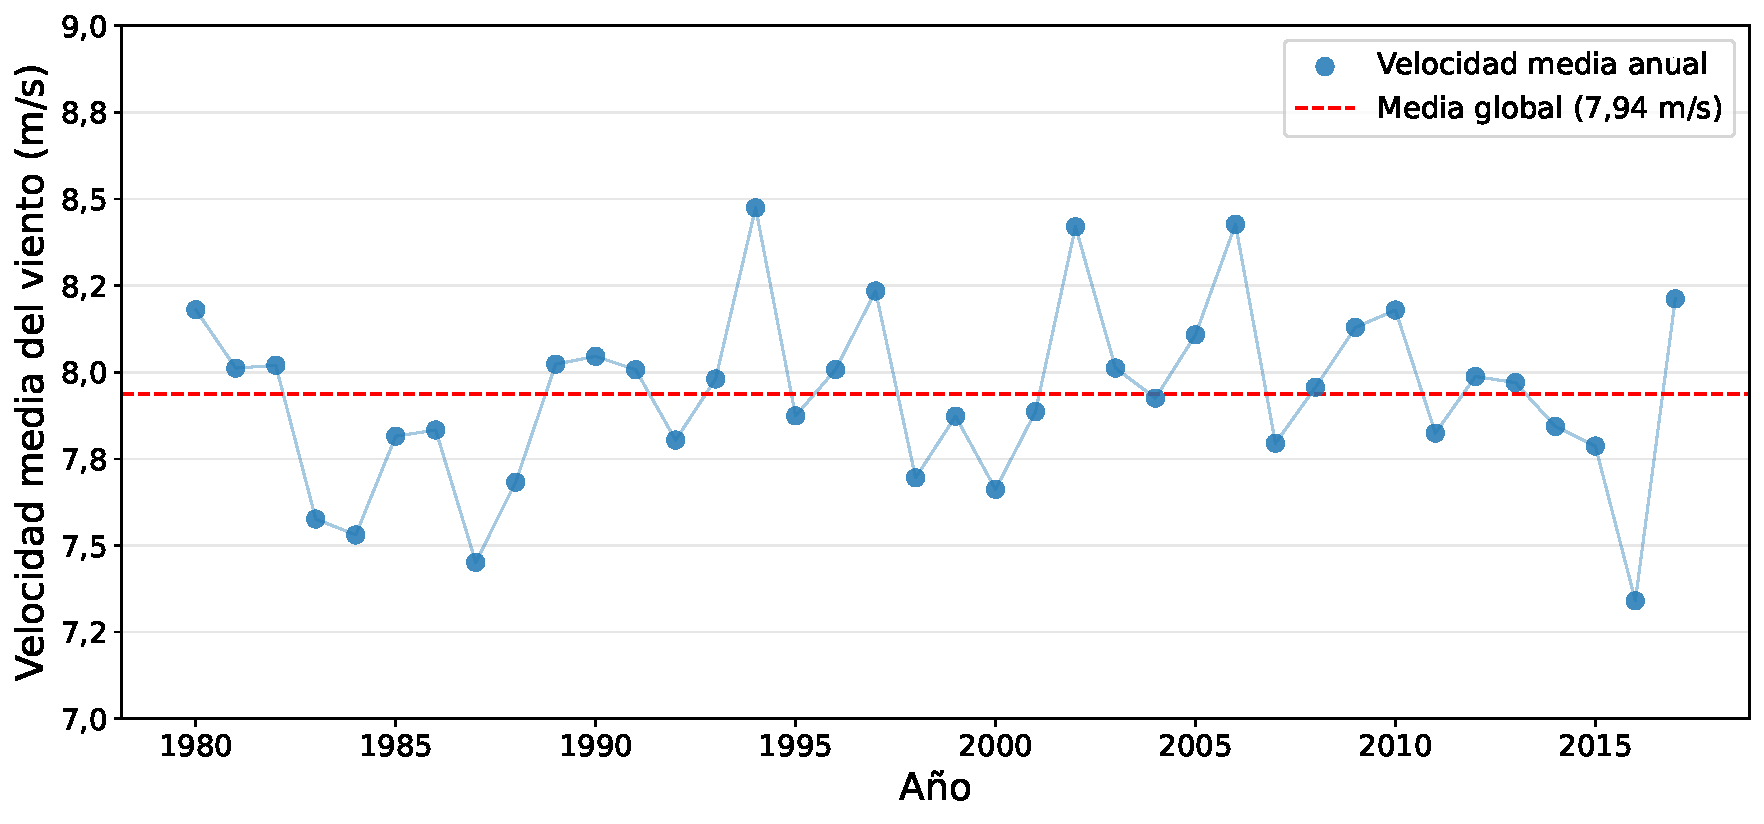
\includegraphics[width=0.7\textwidth]{Figuras/Figuras Resultados/viento_promedio_anual.pdf}
\caption{Velocidad media anual del viento para el periodo 1980--2017.}
\label{fig:viento_promedio_anual}
\end{figure}

La Figura~\ref{fig:viento_promedio_mensual} muestra que los meses de invierno (junio--agosto) presentan velocidades medias superiores a la media anual, mientras que los meses de verano (enero--marzo) registran las velocidades más bajas, con una diferencia estacional cercana al $30\%$.

\begin{figure}[H]
\centering
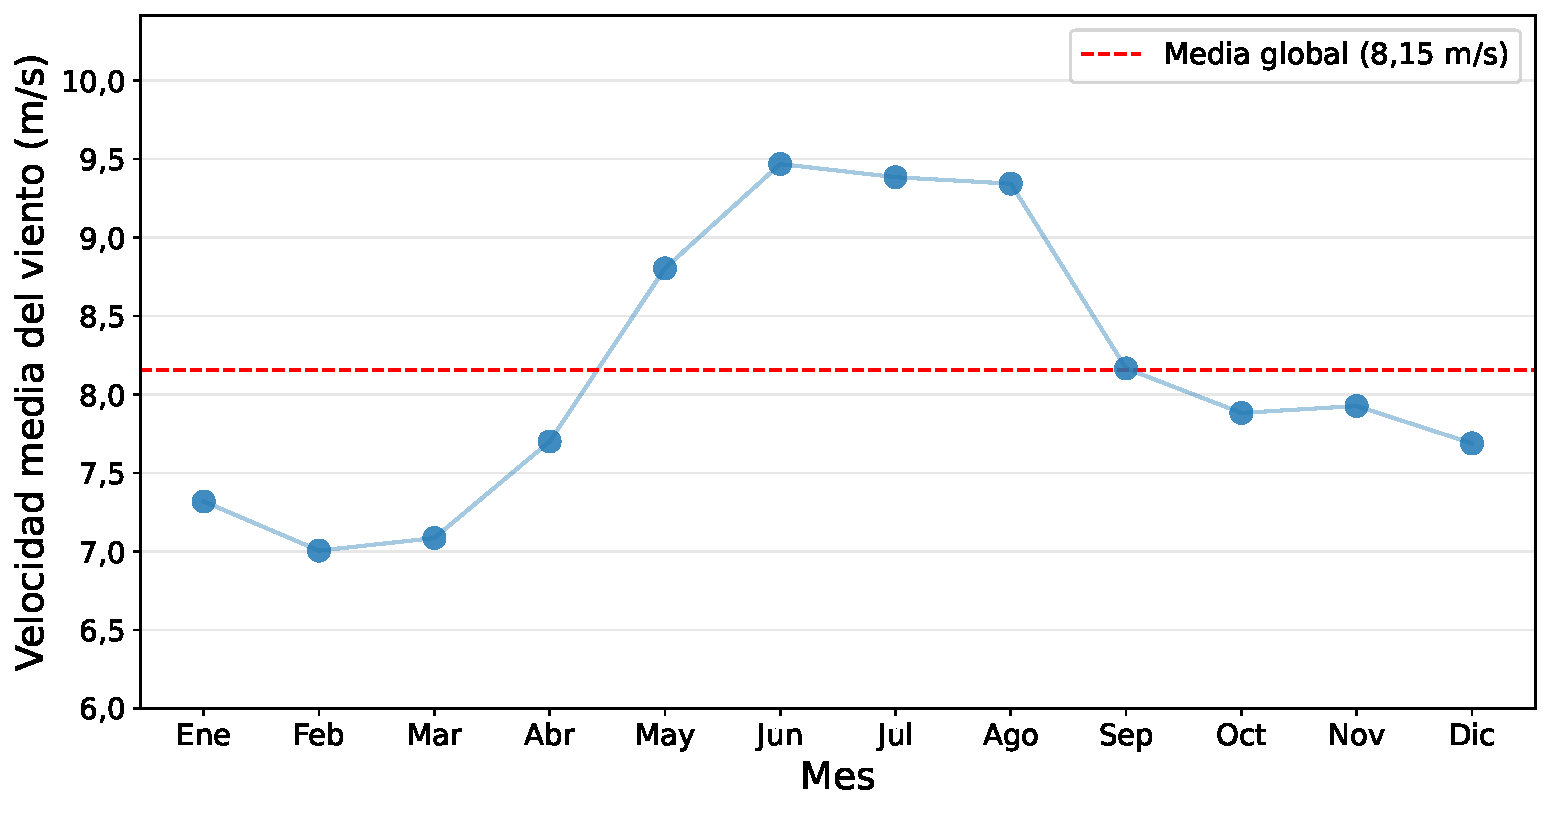
\includegraphics[width=0.7\textwidth]{Figuras/Figuras Resultados/viento_promedio_mensual.pdf}
\caption{Velocidad media mensual del viento para el periodo 1980--2017.}
\label{fig:viento_promedio_mensual}
\end{figure}

La densidad de probabilidad de la velocidad del viento (Figura~\ref{fig:distribucion_viento}) presenta un parámetro de forma $k = 2{,}09$, cercano al caso particular $k = 2$ de la distribución de Rayleigh que la norma adopta como referencia para las clases estándar~\parencite{ennis2018}, y un parámetro de escala $c = 8{,}97$~m/s, ajustados a la altura del centro del rotor, donde la velocidad media resulta en $V_{ave} = 7{,}94$~m/s. El ajuste reproduce la densidad observada con $R^2 = 0{,}970$. Estos dos parámetros reaparecen a lo largo del estudio, ya que la distribución que definen pondera el tiempo de exposición a cada velocidad en el cálculo de fatiga (Sección~\ref{sec:resultados_fatiga}) y entrega la probabilidad de excedencia con que se fija la velocidad de corte.

\begin{figure}[H]
\centering
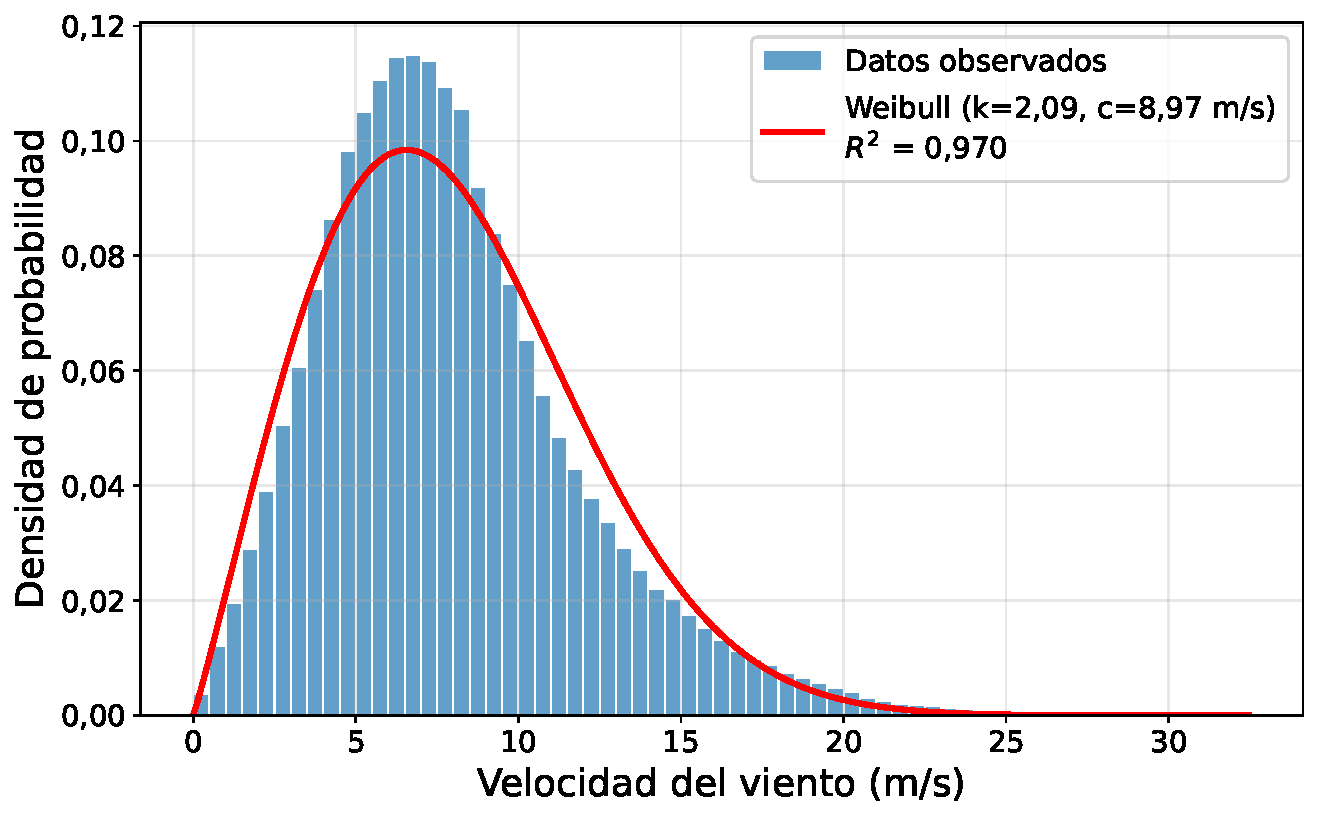
\includegraphics[width=0.7\textwidth]{Figuras/Figuras Resultados/viento_weibull.pdf}
\caption{Densidad de probabilidad y ajuste de Weibull de la velocidad del viento.}
\label{fig:distribucion_viento}
\end{figure}

Con base en esta caracterización, el rango operacional de la turbina se define entre $V_{in} = 2$~m/s y $V_{out} = 25$~m/s. La operación estable a $2$~m/s se verifica mediante las simulaciones LLFVW, que registran producción sostenida y un TSR cercano al óptimo ($C_{p,med} = 0{,}447$, $\lambda = 3{,}88$, Tabla~\ref{tab:curva_potencia}, Sección~\ref{sec:curva_potencia}). El límite superior, adoptado por criterio de diseño (Sección~\ref{sec:control}), tiene un costo marginal en producción, ya que la probabilidad de excedencia del sitio es $P(V > 25\text{ m/s}) = 0{,}02\%$, equivalente a $1{,}75$~h/año, sensiblemente menor a la probabilidad de superar los $20$~m/s, $P(V > 20\text{ m/s}) = 0{,}48\%$ ($42$~h/año). Dado que el coeficiente de potencia decae por debajo de $0{,}06$ para $V \geq 24$~m/s bajo el límite de velocidad de rotación adoptado (Sección~\ref{sec:curva_potencia}), la energía capturable por encima de $25$~m/s resulta despreciable, por lo que las velocidades superiores no se consideran en este estudio.

Las características anteriores del emplazamiento, velocidad media moderada, turbulencia baja y estabilidad interanual sin tendencia de largo plazo, respaldan el uso del registro histórico como representativo del recurso para la estimación de la producción energética.

\section{Caracterización de las propiedades físicas del aire}

Se analizan las temperaturas máximas y mínimas del período 1995--2025, registradas en la estación El Tepual, Puerto Montt (aeropuerto; altitud $85$~m; código DMC $410005$), obtenidas del explorador climático~\parencite{CR2}. Las temperaturas medias mensuales extremas registradas son de 3 \textdegree C para las mínimas y 21 \textdegree C para las máximas (Figura~\ref{fig:climatologia_mensual}).

\begin{figure}[H]
\centering
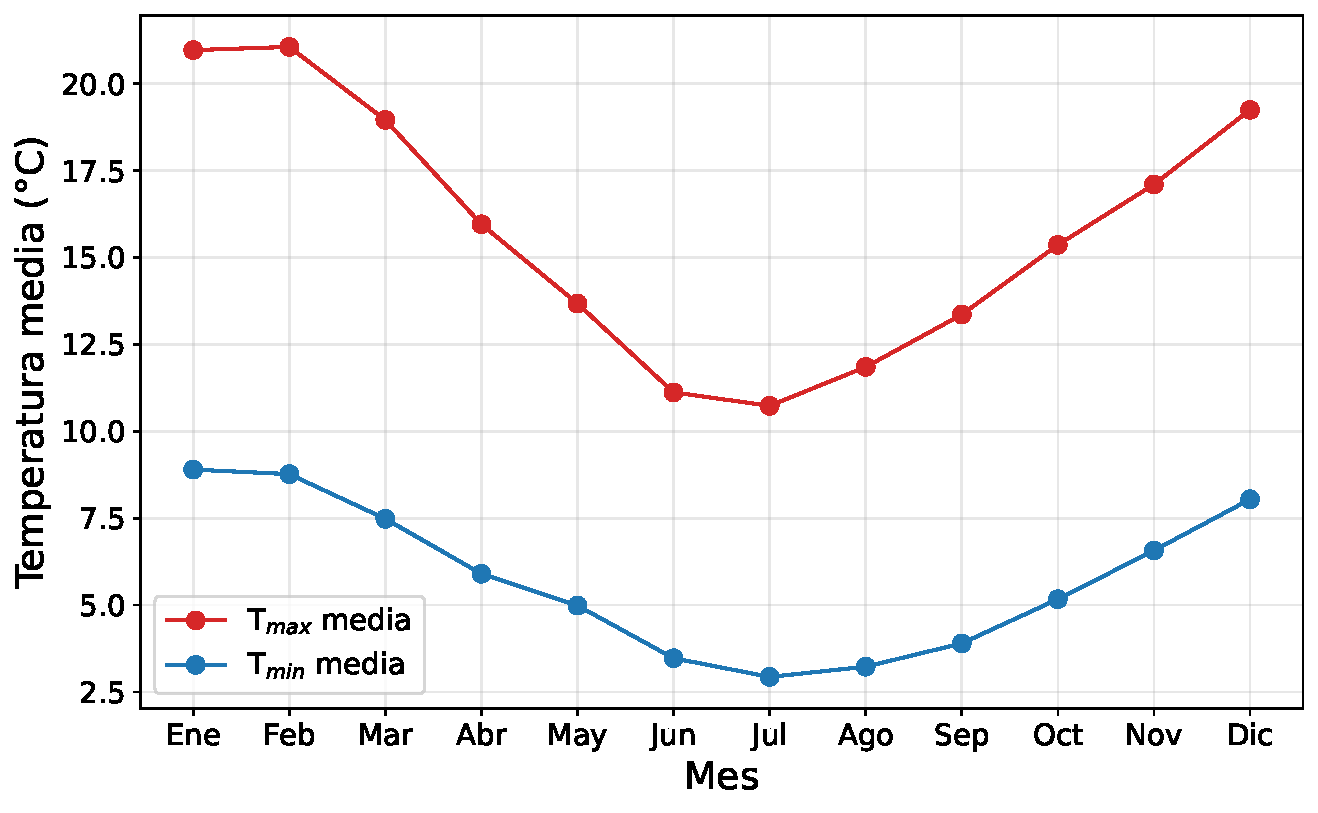
\includegraphics[width=0.6\textwidth]{Figuras/Figuras Resultados/temperatura_climatologia_mensual.pdf}
\caption{Climatología mensual promedio, estación El Tepual, Puerto Montt (1995--2025).}
\label{fig:climatologia_mensual}
\end{figure}

A partir de esta caracterización térmica, se obtienen las propiedades físicas del aire que se resumen en la Tabla~\ref{tab:propiedades_aire}. La variación anual de la viscosidad es inferior al $12\%$, lo que indica que la influencia de la temperatura sobre el número de Reynolds es secundaria respecto a la producida por la variación de la velocidad del viento, efecto que se cuantifica más adelante sobre las fuerzas aerodinámicas (Tabla~\ref{tab:sensibilidad_re}).

\begin{table}[H]
    \centering
    \caption{Propiedades físicas del aire en el emplazamiento, calculadas según las Ecs.~\ref{eq:sutherland}--\ref{eq:visc_cinematica} de la Sección~\ref{sec:propiedades_aire}.}
    \label{tab:propiedades_aire}
    \begin{tabular}{lccc}
        \hline
        \textbf{Propiedad} & \textbf{Símbolo} & \textbf{Valor} & \textbf{Unidad} \\
        \hline
        Viscosidad cinemática mínima & $\nu_{min}$ & $1{,}3535 \times 10^{-5}$ & m$^2$/s \\
        Viscosidad cinemática máxima & $\nu_{max}$ & $1{,}5156 \times 10^{-5}$ & m$^2$/s \\
        Viscosidad cinemática media   & $\bar{\nu}$ & $1{,}4232 \times 10^{-5}$ & m$^2$/s \\
        Densidad media & $\bar{\rho}$ & $1{,}225$ & kg/m$^3$ \\
        \hline
    \end{tabular}
\end{table}

\section{Rango de Reynolds analizado}

La Figura~\ref{fig:reynolds_envelope} presenta la envolvente paramétrica del número de Reynolds en función del ángulo azimutal $\theta$, construida a partir del rango teórico $\lambda \in [2{,}5; 4{,}5]$ y $V \in [2; 25]$~m/s. El $Re_{min} = 2{,}18 \times 10^5$ corresponde a la condición de sotavento a $V = 2$~m/s. La cota superior teórica es $Re_{max} = 5{,}46 \times 10^6$, obtenida a partir de $W_{max} = V_{out} + \Omega R = 70{,}6$~m/s, la simplificación algebraica de la Ec.~\ref{eq:W_theta} para $\theta = 0^\circ$ (Ec.~\ref{eq:W_max}), condición de barlovento en que la velocidad tangencial de la pala se alinea con el viento incidente y ambas magnitudes se suman directamente. Redondeada al millón siguiente, según el criterio de la Sección~\ref{sec:reynolds}, esa cota fija en $6 \times 10^6$ el límite superior adoptado para el cálculo de polares. En cualquier caso, el conjunto de polares calculadas con QFoil ($0{,}35 \times 10^6$ a $6{,}0 \times 10^6$), complementado con las polares experimentales de \textcite{Bianchini2015} para bajo Reynolds ($Re \leq 3 \times 10^5$), cubre completamente las condiciones operacionales simuladas de la turbina.

\begin{figure}[H]
\centering
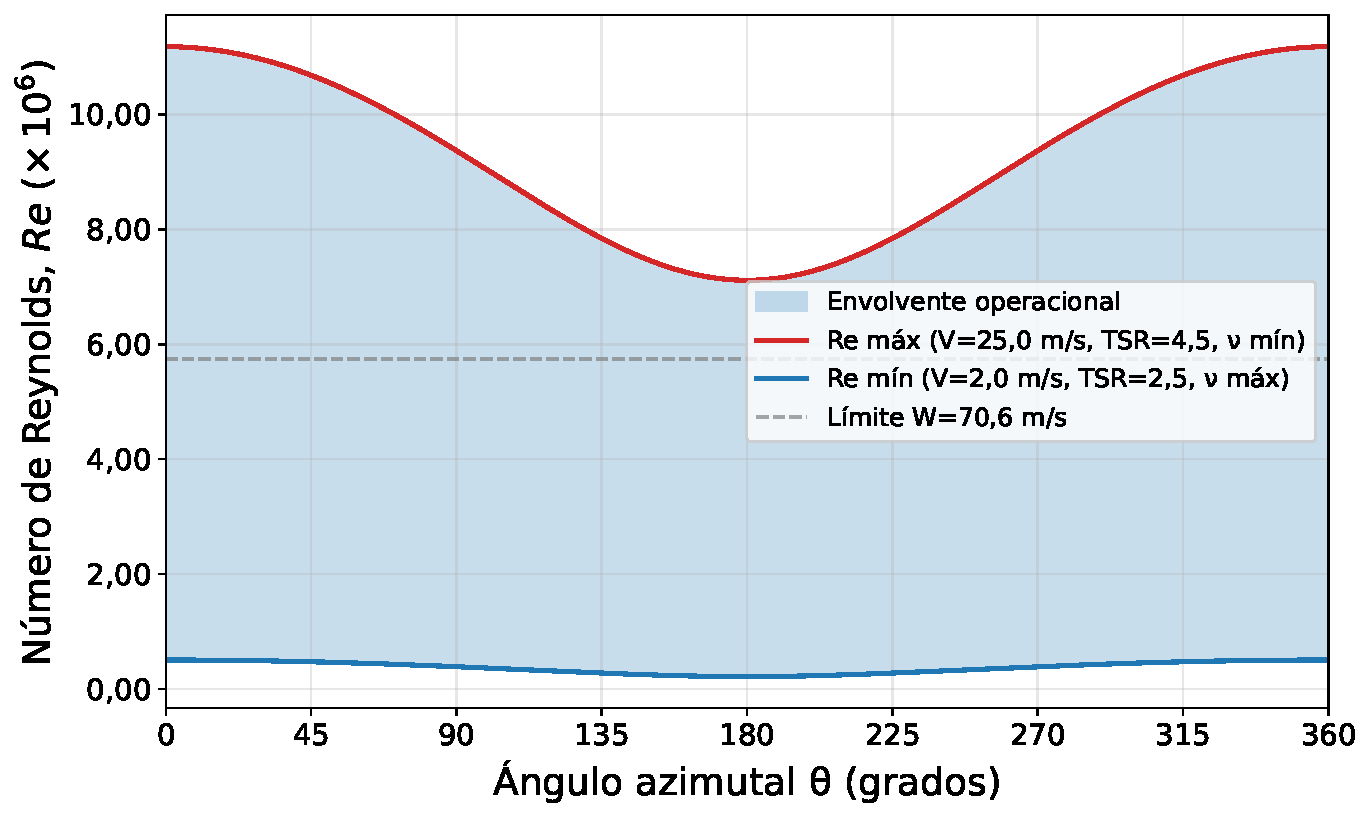
\includegraphics[width=0.75\textwidth]{Figuras/Figuras Resultados/vawt_reynolds_envelope.pdf}
\caption{Envolvente paramétrica del número de Reynolds para el rotor VAWT con perfil NACA 0018.}
\label{fig:reynolds_envelope}
\end{figure}

Esta cobertura resulta particularmente relevante en el extremo superior del rango, donde pequeñas desviaciones en $C_l$ o $C_d$ se amplifican por la dependencia cuadrática de las fuerzas con la velocidad relativa (Ecs.~\ref{eq:fuerza_sustentacion} y~\ref{eq:fuerza_arrastre}).

Esa cobertura absorbe además la incertidumbre que introduce la variabilidad térmica del emplazamiento sobre el Reynolds. Al mantener fija la velocidad relativa $W$, el cociente entre los Reynolds que resultan de evaluar la Ec.~\ref{eq:Re_max_theoretical} con $\nu_{min}$ y con $\nu_{max}$ se reduce al cociente inverso de las viscosidades, según la Ec.~\ref{eq:sensibilidad_re}:

\begin{equation}
    \frac{Re(\nu_{min})}{Re(\nu_{max})} = \frac{Wc/\nu_{min}}{Wc/\nu_{max}} = \frac{\nu_{max}}{\nu_{min}}
    \label{eq:sensibilidad_re}
\end{equation}

de modo que el Reynolds hereda exactamente la misma variación porcentual que la viscosidad. Evaluada en $W_{max} = 70{,}6$~m/s (Sección~\ref{sec:reynolds}), esa variación es de $11{,}98\%$ entre $Re(\nu_{min}) = 5{,}74 \times 10^6$ y $Re(\nu_{max}) = 5{,}12 \times 10^6$, equivalente a $+5{,}2\%$ y $-6{,}1\%$ respecto del $\bar\nu$ adoptado para las simulaciones. Esa magnitud es secundaria frente a la que domina la envolvente de la Figura~\ref{fig:reynolds_envelope}, ya que el rango de $W$ inducido por la velocidad de viento y el TSR analizados abarca un factor de aproximadamente $25$ veces, de $Re_{min} = 2{,}18 \times 10^5$ a $Re_{max} = 5{,}46 \times 10^6$, dos órdenes de magnitud mayor que el efecto térmico.

Las fuerzas de sustentación y arrastre por unidad de envergadura se expresan según las Ecs.~\ref{eq:fuerza_sustentacion} y~\ref{eq:fuerza_arrastre}:

\begin{equation}
    F_L = \frac{1}{2}\rho W^2 c\, C_l(Re,\alpha)
    \label{eq:fuerza_sustentacion}
\end{equation}

\begin{equation}
    F_D = \frac{1}{2}\rho W^2 c\, C_d(Re,\alpha)
    \label{eq:fuerza_arrastre}
\end{equation}

que mantienen $\rho$, $W$ y $c$ fijos frente a este efecto, por lo que su variación porcentual coincide exactamente con la de $C_l$ y $C_d$. La Tabla~\ref{tab:sensibilidad_re} evalúa las polares finales de QFoil ($N_{crit}=7$) entre $Re(\nu_{min})$ y $Re(\nu_{max})$ para ángulos de ataque en régimen adherido, donde $C_l$ varía menos de $0{,}25\%$ y $C_d$ menos de $1{,}2\%$, casi dos órdenes de magnitud menos que el $11{,}98\%$ de variación del propio Reynolds. La influencia de la temperatura sobre las fuerzas predichas resulta, por tanto, despreciable frente a la que ejerce la velocidad del viento, y por extensión sobre el coeficiente de potencia y las cargas estructurales derivadas en las secciones siguientes, lo que refuerza la confiabilidad de las cargas señalada anteriormente.

\begin{table}[H]
    \centering
    \caption{Variación de $C_l$ y $C_d$ del NACA 0018 entre $Re(\nu_{min}) = 5{,}74 \times 10^6$ y $Re(\nu_{max}) = 5{,}12 \times 10^6$, respecto del valor a $\bar\nu$, para ángulos de ataque en régimen adherido.}
    \label{tab:sensibilidad_re}
    \begin{tabular}{ccccc}
        \hline
        \textbf{$\alpha$ (°)} & \textbf{$\Delta C_l(\nu_{min})$} & \textbf{$\Delta C_l(\nu_{max})$} & \textbf{$\Delta C_d(\nu_{min})$} & \textbf{$\Delta C_d(\nu_{max})$} \\
        \hline
        $5$  & $+0{,}11\%$ & $-0{,}13\%$ & $-0{,}33\%$ & $+0{,}55\%$ \\
        $8$  & $+0{,}13\%$ & $-0{,}18\%$ & $-0{,}49\%$ & $+0{,}76\%$ \\
        $10$ & $+0{,}19\%$ & $-0{,}25\%$ & $-0{,}78\%$ & $+0{,}97\%$ \\
        $12$ & $+0{,}18\%$ & $-0{,}21\%$ & $-0{,}96\%$ & $+1{,}14\%$ \\
        \hline
    \end{tabular}
\end{table}

\section{Resultados de la caracterización y extrapolación de perfiles}

Esta sección presenta los resultados de la caracterización aerodinámica del perfil NACA 0018, comenzando por el análisis de sensibilidad que fija el parámetro de transición de QFoil, seguido de las polares finales adoptadas para las simulaciones y de su comparación con datos experimentales.

\subsection{Análisis de sensibilidad al parámetro de transición}

En la Figura~\ref{fig:comparacion_ncrit_250k} se presentan las curvas polares calculadas con QFoil para el perfil NACA 0018 a $Re = 2{,}5 \times 10^5$, considerando los seis valores de $N_{crit}$ simulados, junto con los datos experimentales de \textcite{Bianchini2015} para el mismo número de Reynolds. La figura incluye los coeficientes de determinación $R^2$ del ajuste de $C_l$ respecto a los datos experimentales, evaluados en la región pre-stall ($\alpha \in [-5^\circ, 10^\circ]$), donde el modelo QFoil representa adecuadamente el comportamiento lineal del perfil. Los valores posteriores a la pérdida no son representativos, ya que los códigos de capa límite integral pierden validez cuando la separación se vuelve masiva (Sección~\ref{sec:polares}), y se modelan más adelante en QBlade mediante la extrapolación de Montgomerie de la Sección~\ref{sec:montgomerie_resultados}.

En la curva de sustentación se distinguen tres regiones. Hasta aproximadamente $10^\circ$ el $C_l$ crece de forma prácticamente lineal con el ángulo de ataque y las seis curvas calculadas se superponen con los datos experimentales, lo que se refleja en los valores de $R^2$ cercanos a la unidad. Entre $10^\circ$ y $15^\circ$ la pendiente se aplana y las curvas empiezan a separarse entre sí según el $N_{crit}$ adoptado. La tercera región corresponde a la pérdida, que en los datos experimentales ocurre de forma abrupta en $\alpha = 15{,}6^\circ$, donde el $C_l$ cae de $1{,}03$ a $0{,}49$, mientras que las curvas de QFoil no reproducen esa caída y siguen creciendo hasta $1{,}06$ en $\alpha = 20^\circ$ con $N_{crit} = 7$. La pérdida aparece por tanto antes en los datos experimentales que en las polares calculadas, lo que es esperable en esta etapa, ya que la figura corresponde a la salida directa de QFoil, todavía sin el ajuste de pérdida profunda que se calibra en la Sección~\ref{sec:montgomerie_resultados}.

La elección de $N_{crit}$ tiene un efecto directo sobre la predicción de cargas aerodinámicas. Un valor bajo ($N_{crit} = 4$) fuerza la transición temprana de capa límite, lo que reduce el $C_l$ máximo y subestima las cargas en la zona de stall. Por el contrario, un valor alto ($N_{crit} \geq 11$) retrasa la transición, permitiendo que el flujo permanezca laminar más allá de lo físicamente realista en un entorno operacional, ya que ese rango corresponde a flujos prácticamente libres de perturbaciones (Tabla~\ref{tab:ncrit_values}), y produce una sobrestimación creciente de $C_l$. Ambos efectos son los que documenta \textcite{drela1989xfoil} para el criterio $e^N$, descrito en la Sección~\ref{sec:polares}, y los que se observan en la figura. El valor $N_{crit} = 7$ se sitúa dentro del rango correspondiente a túnel de viento turbulento según la documentación de Xfoil~\parencite{drela1989xfoil}, condición más representativa del ambiente marino en que opera la turbina que los valores $N_{crit} \geq 9$ (túnel de viento limpio o promedio), y es el que mejor reproduce los datos experimentales en la región pre-stall ($R^2 = 0{,}9950$). Por estas razones, $N_{crit} = 7$ es seleccionado como parámetro de configuración para todas las simulaciones aerodinámicas.

\begin{figure}[H]
\centering
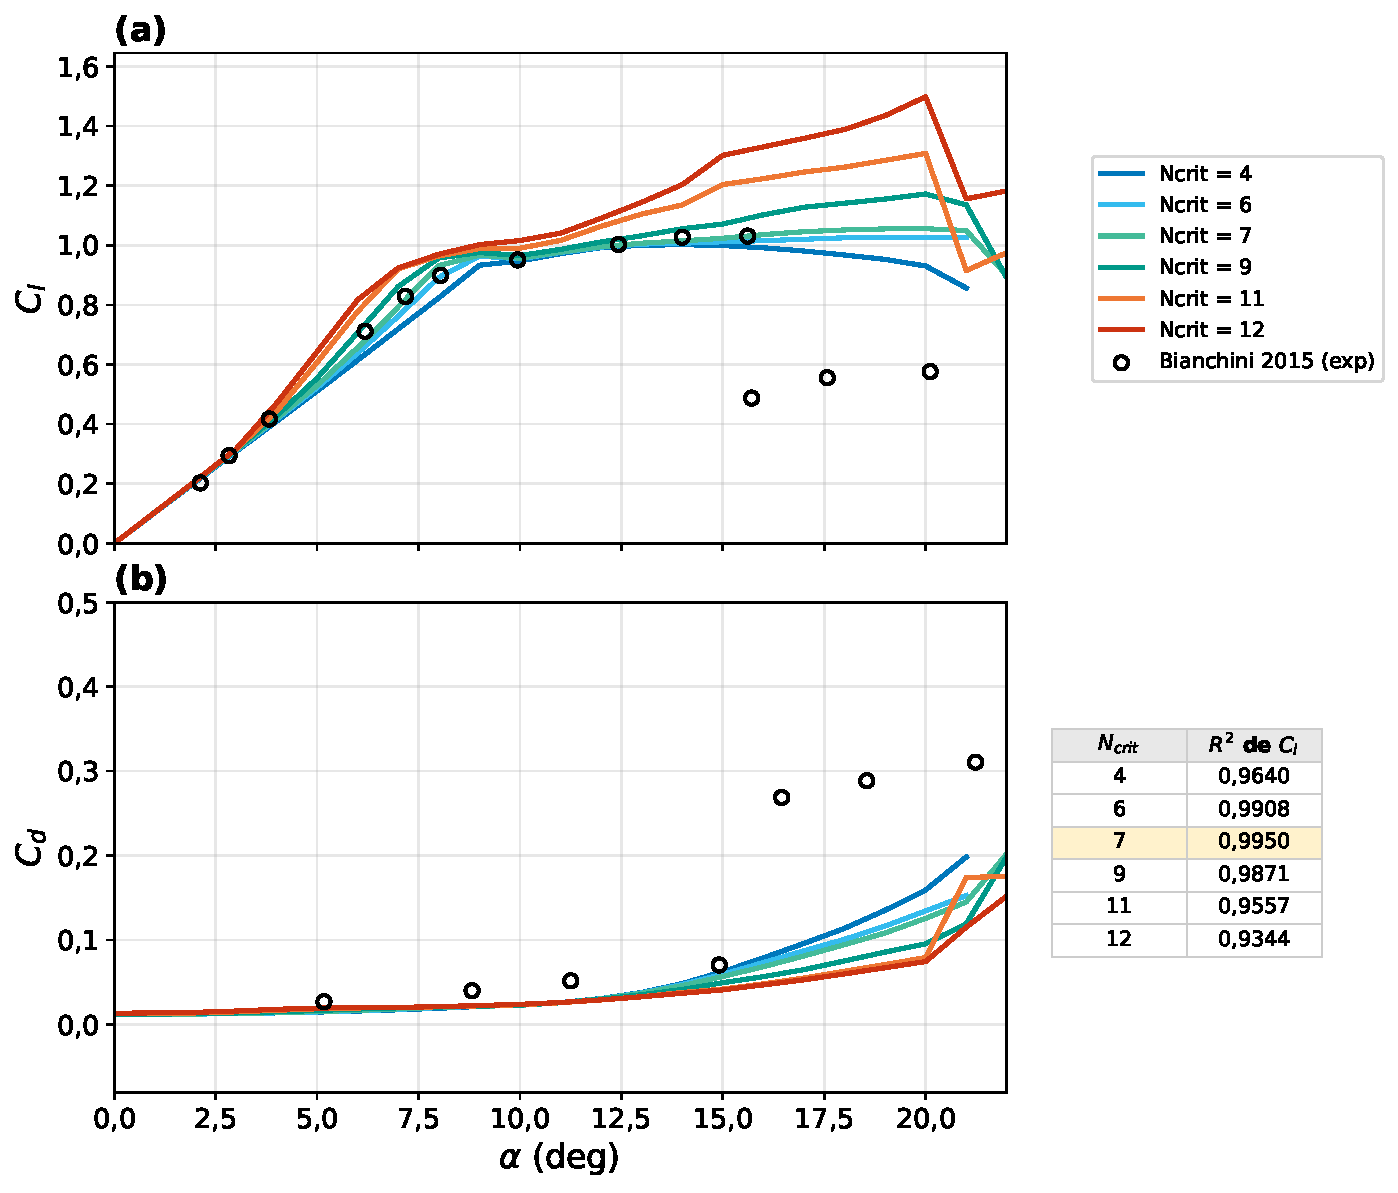
\includegraphics[width=0.9\textwidth]{Figuras/Figuras Resultados/comparacion_vs_experimental_250k.pdf}
\caption{Comparación de polares del perfil NACA 0018 para distintos valores del criterio de transición, $Re = 2{,}5 \times 10^5$: (a) Sustentación y (b) Arrastre.}
\label{fig:comparacion_ncrit_250k}
\end{figure}

\subsection{Polares calculadas}

Las curvas polares calculadas con QFoil para 42 números de Reynolds entre $Re = 0{,}35 \times 10^6$ y $6 \times 10^6$ para el perfil NACA 0018 se presentan en las Figuras~\ref{fig:naca_cl} y~\ref{fig:naca_cd}. El incremento del $38\%$ en $C_{l,max}$ a lo largo del rango de Reynolds, desde $1{,}05$ hasta $1{,}45$, es esperable, ya que a mayor número de Reynolds la capa límite dispone de más energía cinética para resistir el gradiente adverso de presión, retrasando la separación~\parencite{White2006,Anderson2016}. Simultáneamente, la disminución del coeficiente de arrastre en la región pre-stall refleja la reducción del espesor relativo de la capa límite~\parencite{White2006}. El ángulo de stall se mantiene aproximadamente constante en $14^\circ$--$15^\circ$, comportamiento característico de perfiles simétricos NACA de la serie 00XX a números de Reynolds moderados, donde la separación está dominada por el gradiente de presión más que por efectos viscosos~\parencite{Anderson2016}.

\label{sec:montgomerie_resultados}Estas curvas ya incorporan la extrapolación angular a todo el rango que recorre la pala en una revolución completa ($360^\circ$), mediante el modelo de \textcite{montgomerie2004methods} configurado en QBlade con los criterios descritos en la Sección~\ref{sec:extrapolacion_polares}. El coeficiente de arrastre a 90° se fija en $C_{d90} = 1{,}83$ a partir de los datos experimentales de \textcite{Bianchini2015} para el perfil NACA 0018 a $Re = 2{,}5 \times 10^5$.

\begin{figure}[H]
\centering
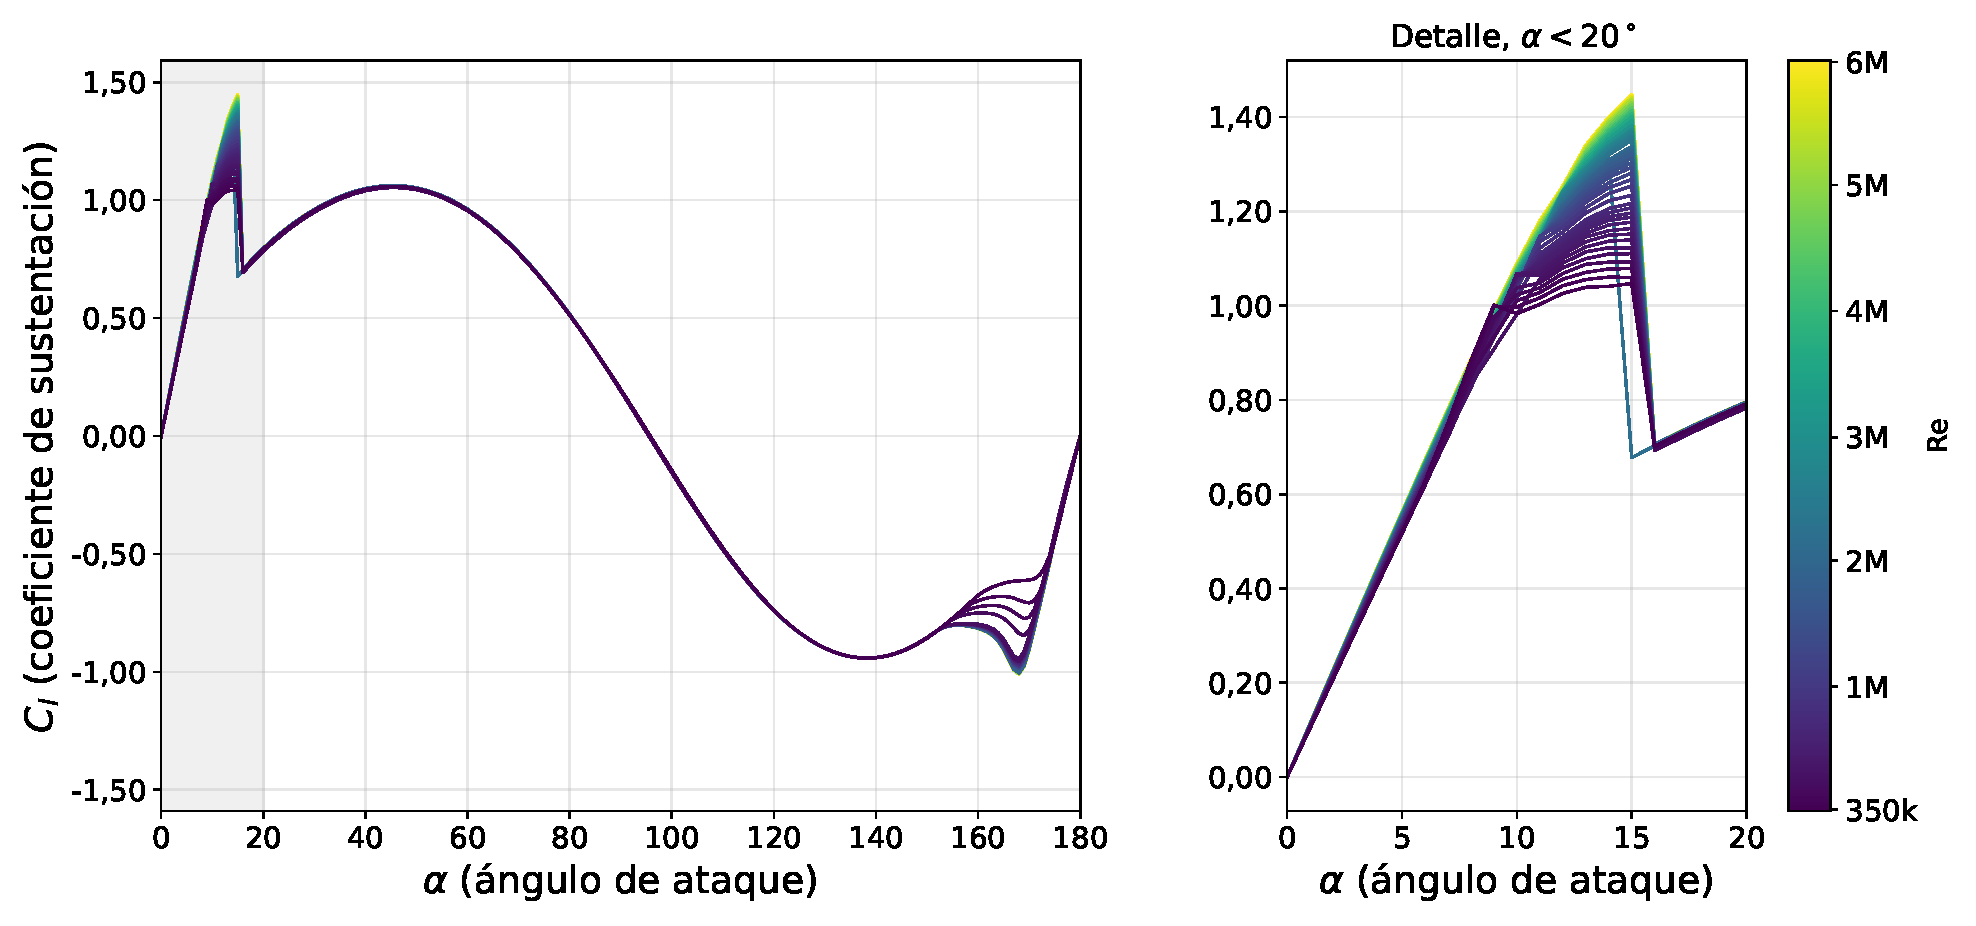
\includegraphics[width=1\textwidth]{Figuras/Figuras Resultados/NACA0018_CL_vs_AoA.pdf}
\caption{Coeficiente de sustentación sobre $\alpha$ del perfil NACA 0018 para diferentes números de Reynolds, $N_{crit}=7$, obtenido mediante QFoil con extrapolación de Montgomerie.}
\label{fig:naca_cl}
\end{figure}

\begin{figure}[H]
\centering
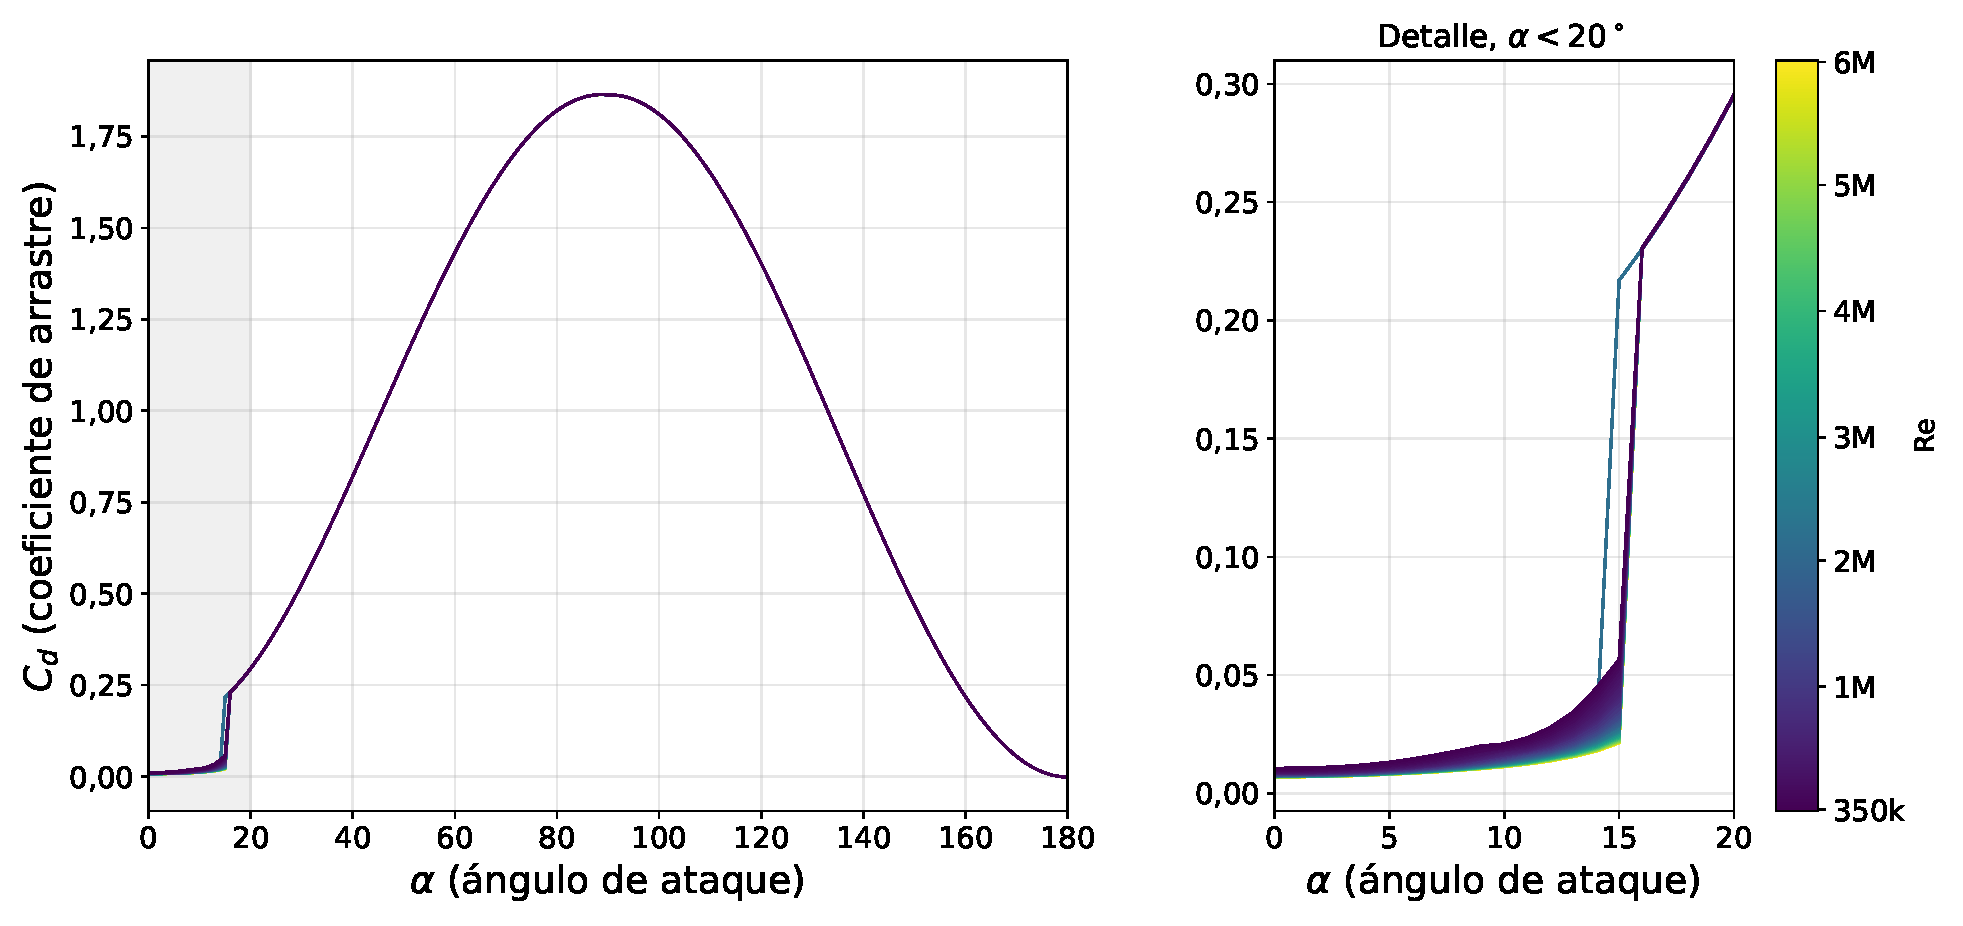
\includegraphics[width=1\textwidth]{Figuras/Figuras Resultados/NACA0018_CD_vs_AoA.pdf}
\caption{Coeficiente de arrastre sobre $\alpha$ del perfil NACA 0018 para diferentes números de Reynolds, $N_{crit}=7$, obtenido mediante QFoil con extrapolación de Montgomerie.}
\label{fig:naca_cd}
\end{figure}

\subsection{Comparación con datos experimentales}

La Figura~\ref{fig:sheldahl_bianchini_qfoil} presenta la comparación entre tres fuentes independientes de datos aerodinámicos para el perfil NACA 0018 en el rango $0^\circ$ a $180^\circ$: las curvas de \textcite{Sheldahl1981}, los datos experimentales de \textcite{Bianchini2015} para $Re = 6 \times 10^4$ a $3 \times 10^5$, y cinco polares representativas calculadas con QFoil ($N_{crit} = 7$) desde $Re = 3{,}5 \times 10^5$ hasta $Re = 5 \times 10^6$. La coincidencia entre las tres fuentes en las zonas de solapamiento de Reynolds es estrecha en la región pre-stall, donde QFoil se desvía de Bianchini menos de un $3\%$ en $C_l$ para $\alpha \geq 8^\circ$, mientras que Sheldahl se aparta hasta un $13\%$, coherente con las deficiencias de esa base de datos histórica señaladas en la Sección~\ref{sec:caracterizacion_aero}. En la región de pérdida profunda, entre $150^\circ$ y $180^\circ$, las diferencias entre Sheldahl y Bianchini alcanzan hasta $0{,}33$ en $C_l$, magnitud comparable a las discrepancias que los propios \textcite{Bianchini2015} reportan en esa misma zona angular al contrastar sus mediciones con sus simulaciones CFD (Sección~\ref{sec:caracterizacion_aero}). Esta coincidencia constituye una validación cruzada entre un método computacional (panel con capa límite integral), datos experimentales recientes y la referencia histórica del perfil. Las polares de Bianchini cubren el rango de bajo Reynolds ($Re \leq 3 \times 10^5$) donde QFoil no alcanza convergencia, complementando así el conjunto de datos requerido para las simulaciones en todo el rango operacional de la turbina.

\begin{figure}[H]
\centering
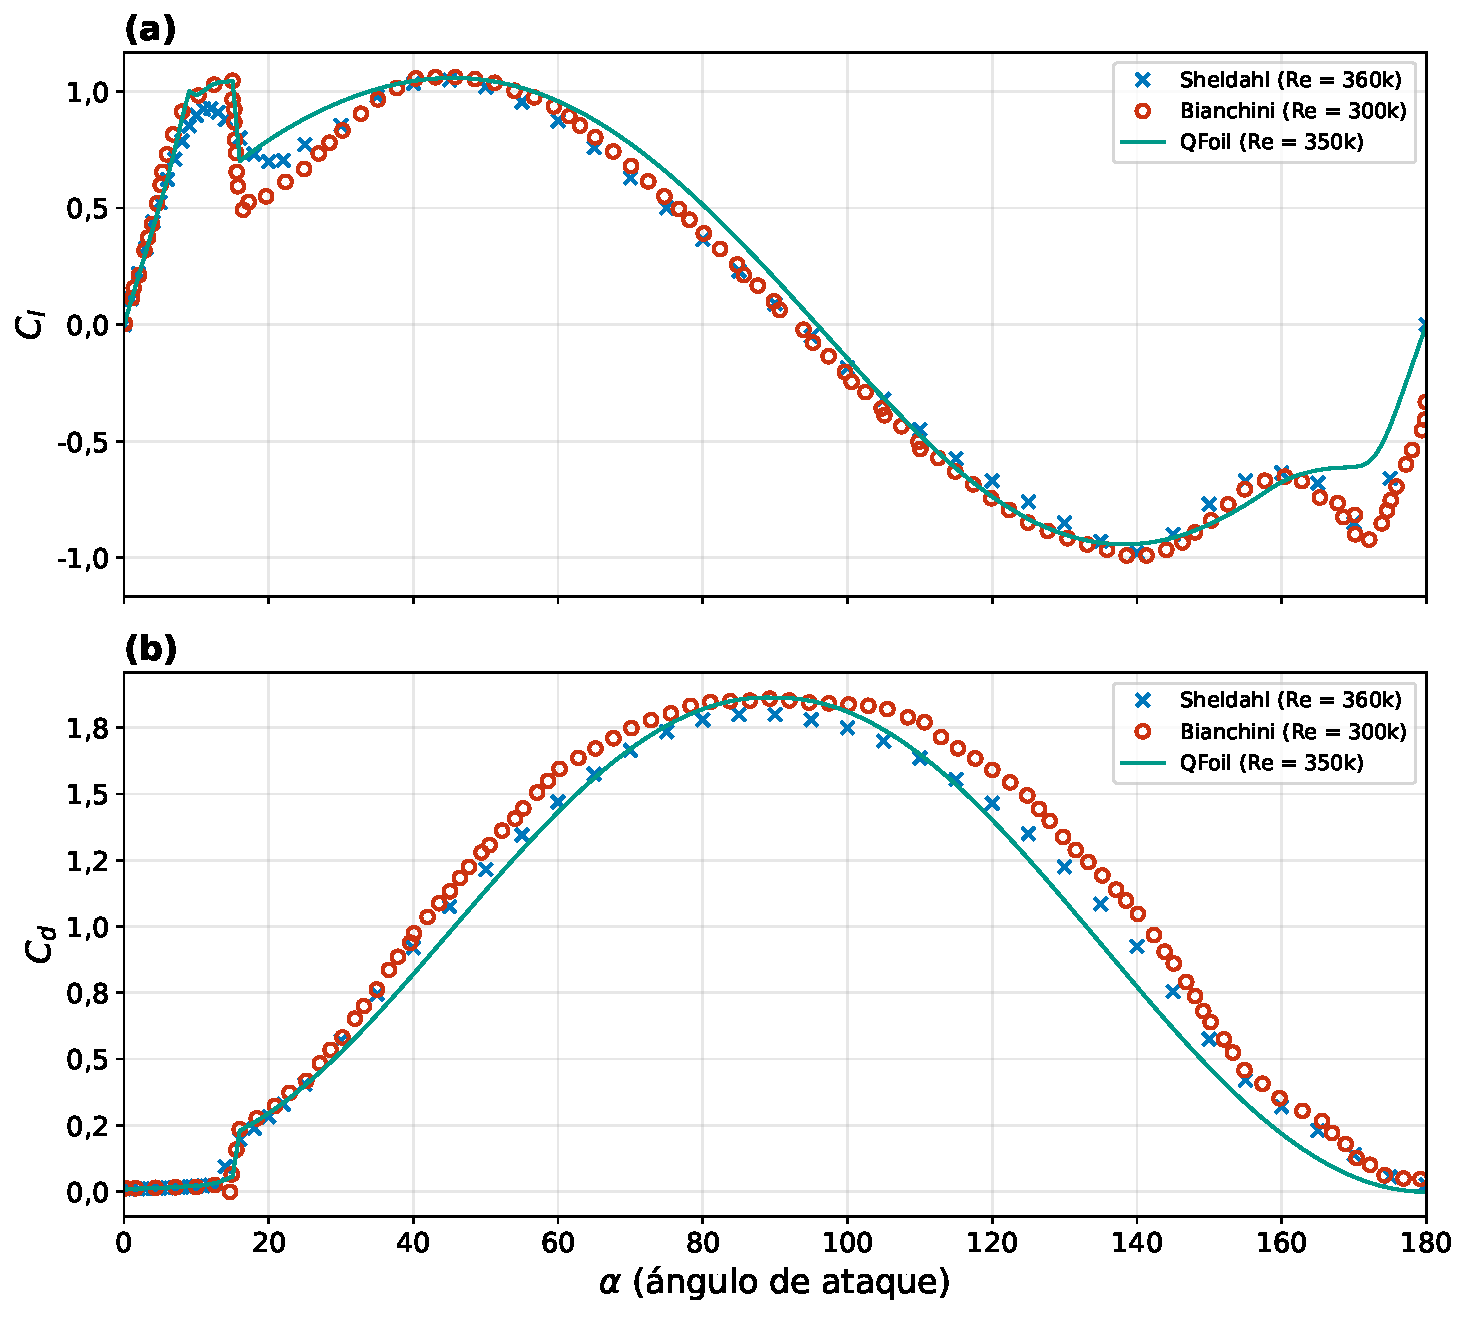
\includegraphics[width=0.85\textwidth]{Figuras/Figuras Resultados/Sheldahl_vs_Bianchini_vs_QFoil.pdf}
\caption{(a) Coeficiente de sustentación $C_l$ y (b) coeficiente de arrastre $C_d$ del perfil NACA 0018, comparando \textcite{Sheldahl1981}, \textcite{Bianchini2015} y QFoil.}
\label{fig:sheldahl_bianchini_qfoil}
\end{figure}

Una vez calibrado el modelo aerodinámico del perfil, la siguiente etapa consiste en caracterizar el desempeño del rotor completo. Antes de ejecutar las simulaciones aerodinámicas de alta fidelidad (LLFVW), se realiza un barrido paramétrico mediante DMST para identificar la relación de velocidad de punta que maximiza la extracción de potencia. El $\lambda_{opt}$ así obtenido se utiliza como condición de referencia para la estrategia de control en las simulaciones LLFVW definitivas.

\section{Relación de velocidad de punta óptima}
\label{sec:tsr_optimo}

La Figura~\ref{fig:dmst_cp_vs_tsr} presenta las curvas TSR vs $C_p$ obtenidas mediante DMST para el rango de velocidades operacionales entre $V_{in} = 2$ m/s y $V_{out} = 25$ m/s. El valor máximo de $C_p$ se alcanza a un $\lambda_{opt} = 3{,}80$, con un $C_{p,max} = 0{,}5736$. Este valor supera el rango validado experimentalmente para configuraciones H-Darrieus ($0{,}35$--$0{,}45$)~\parencite{Essahraoui2026}, en aproximadamente un $27{,}5\%$ sobre el límite superior del rango, sobreestimación sistemática que corresponde a la limitación del método DMST descrita en la Sección~\ref{sec:metodos_aerodinamicos}~\parencite{Essahraoui2026,Islam2008}.

\begin{figure}[H]
    \centering
    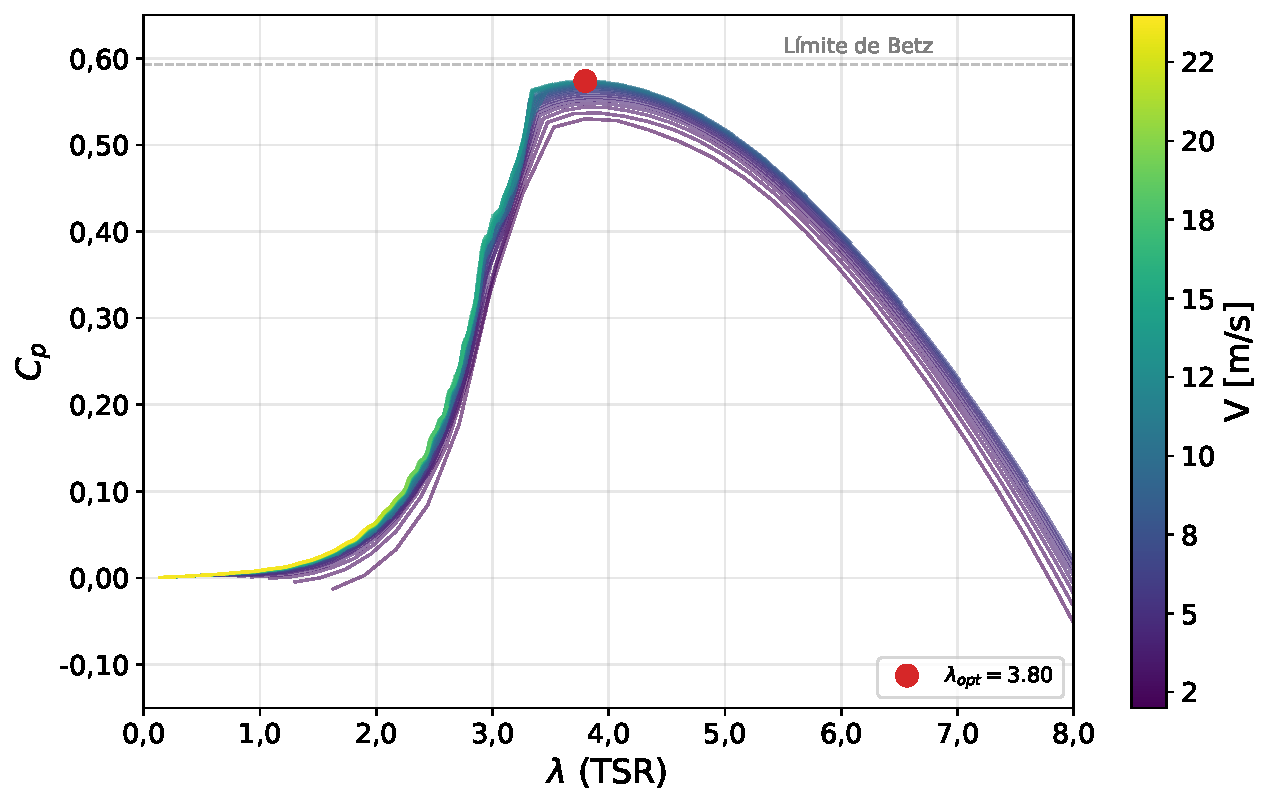
\includegraphics[width=0.75\textwidth]{Figuras/Figuras Resultados/dmst_cp_vs_tsr.pdf}
    \caption{Curvas TSR vs $C_p$ obtenidas mediante DMST para el rango operacional de velocidades de viento, coloreadas según $V$.}
    \label{fig:dmst_cp_vs_tsr}
\end{figure}

La posición del óptimo, en cambio, cuenta con un respaldo independiente del método, ya que la solidez del rotor, $\sigma = Nc/R = 0{,}3184$, se sitúa dentro del rango $0{,}25$--$0{,}35$ que \textcite{Essahraoui2026} reportan como óptimo para H-rotores de tres palas con perfiles simétricos NACA, a partir de los resultados de \textcite{Subramanian2017}, si bien los propios autores advierten que dicho óptimo se desplaza con el perfil, el número de Reynolds y el TSR objetivo. Como se establece en la Sección~\ref{sec:solidez}, este parámetro permite aproximar la posición del máximo de $C_p$ en función del TSR, ya que rotores de baja solidez operan a TSR elevados ($\lambda > 4$) y rotores de alta solidez lo hacen a TSR bajos ($\lambda \approx 2$--$3$). La solidez del rotor estudiado es intermedia entre ambos regímenes, por lo que cabe esperar que su $\lambda_{opt}$ también lo sea, situado entre esos dos extremos; el valor obtenido mediante el barrido DMST, $\lambda_{opt} = 3{,}80$, cae precisamente en ese intervalo intermedio. Esta correspondencia constituye una verificación independiente del resultado, porque la solidez es un parámetro puramente geométrico que no depende del método aerodinámico con que se simula el rotor, de modo que la posición del óptimo que predice, a partir de la relación empírica documentada en la literatura, no hereda el sesgo del DMST señalado en el párrafo anterior. Que ambas vías, la curva TSR vs $C_p$ del barrido DMST y la relación solidez-TSR de la literatura, apunten a la misma posición del óptimo respalda el valor $\lambda_{opt} = 3{,}80$ con independencia de esas limitaciones, aunque estas sí afecten la magnitud de $C_{p,max}$ estimada, como se señala más arriba. Sobre esta base, dicho valor se adopta como TSR de referencia para las simulaciones LLFVW.

Con el \gls{tsr} determinado queda fijada también la consigna de velocidad máxima de rotación. Aplicando el criterio de la Sección~\ref{sec:criterio_rotacion} con $\lambda = 3{,}80$ y la velocidad de viento nominal de $12$~m/s se obtiene la Ec.~\ref{eq:omega_diseno}:

\begin{equation}
    \Omega = \frac{\lambda \, V}{R} = \frac{3{,}8 \times 12}{10{,}365} = 4{,}398\ \text{rad/s} = 42{,}0\ \text{rpm}
    \label{eq:omega_diseno}
\end{equation}

El mismo criterio, aplicado a la T1-turbine ($R = 13$~m), reproduce su límite documentado de $33$~rpm con un error del $1{,}5\%$~\parencite{Mollerstrom2017}, lo que respalda la consigna adoptada. La velocidad de punta que de ella resulta, $V_{tip} = \Omega R = 45{,}6$~m/s, equivale a $\lambda V$ y es por tanto independiente del radio, por lo que coincide con la que se obtiene para la T1-turbine a partir de los parámetros de la Tabla~\ref{tab:t1_params}.

\section{Simulación aerodinámica de la turbina}
\label{sec:curva_potencia}

Con el TSR óptimo determinado y las polares validadas, se procede a la simulación aerodinámica del rotor. A diferencia del barrido DMST, que opera sobre promedios estacionarios, las simulaciones LLFVW resuelven la interacción dinámica entre el campo de viento turbulento y la estela tridimensional que el rotor genera~\parencite{marten2019qblade}.

Los parámetros operacionales de la Tabla~\ref{tab:curva_potencia} corresponden al promedio temporal de cada una de las 72 simulaciones LLFVW (Sección~\ref{sec:velocidades_simulacion}), descartado el transitorio inicial, y promediado a su vez sobre las $6$ semillas por velocidad de viento.

\begin{table}[H]
    \centering
    \caption{Parámetros operacionales promedio de la turbina por velocidad de viento ($\Delta\theta = 5^\circ$, $N = 6$ semillas por velocidad).}
    \label{tab:curva_potencia}
    \begin{tabular}{lcccc}
        \hline
        $V$ (m/s) & RPM & TSR & $P_{med}$ (kW) & $C_{p,med}$ \\
        \hline
        $2$  & $6{,}7$  & $3{,}882$ & $1{,}0$    & $0{,}447$ \\
        $4$  & $13{,}6$ & $3{,}853$ & $8{,}5$    & $0{,}452$ \\
        $6$  & $20{,}0$ & $3{,}734$ & $26{,}3$   & $0{,}438$ \\
        $8$  & $26{,}6$ & $3{,}701$ & $61{,}7$   & $0{,}431$ \\
        $10$ & $33{,}3$ & $3{,}667$ & $121{,}4$  & $0{,}421$ \\
        $12$ & $39{,}5$ & $3{,}698$ & $201{,}5$  & $0{,}432$ \\
        $14$ & $42{,}0$ & $3{,}078$ & $349{,}8$  & $0{,}437$ \\
        $16$ & $42{,}0$ & $2{,}689$ & $485{,}0$  & $0{,}422$ \\
        $18$ & $42{,}0$ & $2{,}391$ & $503{,}4$  & $0{,}327$ \\
        $20$ & $42{,}0$ & $2{,}152$ & $423{,}5$  & $0{,}205$ \\
        $22$ & $42{,}0$ & $1{,}956$ & $369{,}3$  & $0{,}137$ \\
        $24$ & $42{,}0$ & $1{,}793$ & $336{,}3$  & $0{,}094$ \\
        \hline
    \end{tabular}
\end{table}

La progresión de la velocidad de rotación confirma el funcionamiento de la estrategia de control y delimita dos regímenes de operación. Por debajo de $12$~m/s la ley $K$-$\omega^2$ acelera el rotor de forma aproximadamente proporcional al viento~\parencite{Johnson2006}, con lo que el TSR se mantiene entre $3{,}67$ y $3{,}88$, en torno al $\lambda_{opt} = 3{,}80$ de diseño. A partir de $14$~m/s la rotación alcanza su límite de $42$~rpm y permanece en él, mientras el TSR decae hasta $1{,}79$ a $24$~m/s, alejando el punto de operación del óptimo aerodinámico.

Estas simulaciones permiten además verificar a posteriori la validez de las polares empleadas, ya que el número de Reynolds máximo que registran, $Re_{max} = 5{,}94 \times 10^6$ a $V = 24$~m/s, es coherente con la cota teórica de $5{,}46 \times 10^6$ de la Sección~\ref{sec:reynolds}, y la diferencia proviene de las fluctuaciones instantáneas de velocidad inducidas por la turbulencia. Ambos valores quedan cubiertos por el rango de polares adoptado, por lo que en ningún instante se extrapolan datos aerodinámicos fuera del dominio caracterizado.

La Figura~\ref{fig:curva_potencia} presenta la potencia media y el coeficiente de potencia promedio de las simulaciones LLFVW en función de la velocidad de viento. Ambas curvas reproducen los dos regímenes descritos, ya que la potencia aumenta de forma sostenida hasta un máximo de $503{,}4$~kW a $V = 18$~m/s y disminuye después hasta $336{,}3$~kW a $V = 24$~m/s, mientras que el coeficiente de potencia se mantiene en una meseta de $0{,}42$--$0{,}45$ hasta $V = 16$~m/s, con el rotor operando en torno a $\lambda_{opt}$, y decae hasta $0{,}094$ a $V = 24$~m/s una vez alcanzado el límite de velocidad de rotación. La línea discontinua en la Figura~\ref{fig:curva_potencia}b indica el límite de Betz, la fracción máxima de energía cinética que un rotor puede extraer según la teoría del disco actuador, $C_{p,Betz} = 16/27 \approx 0{,}593$~\parencite{Paraschivoiu2002}.

\begin{figure}[H]
    \centering
    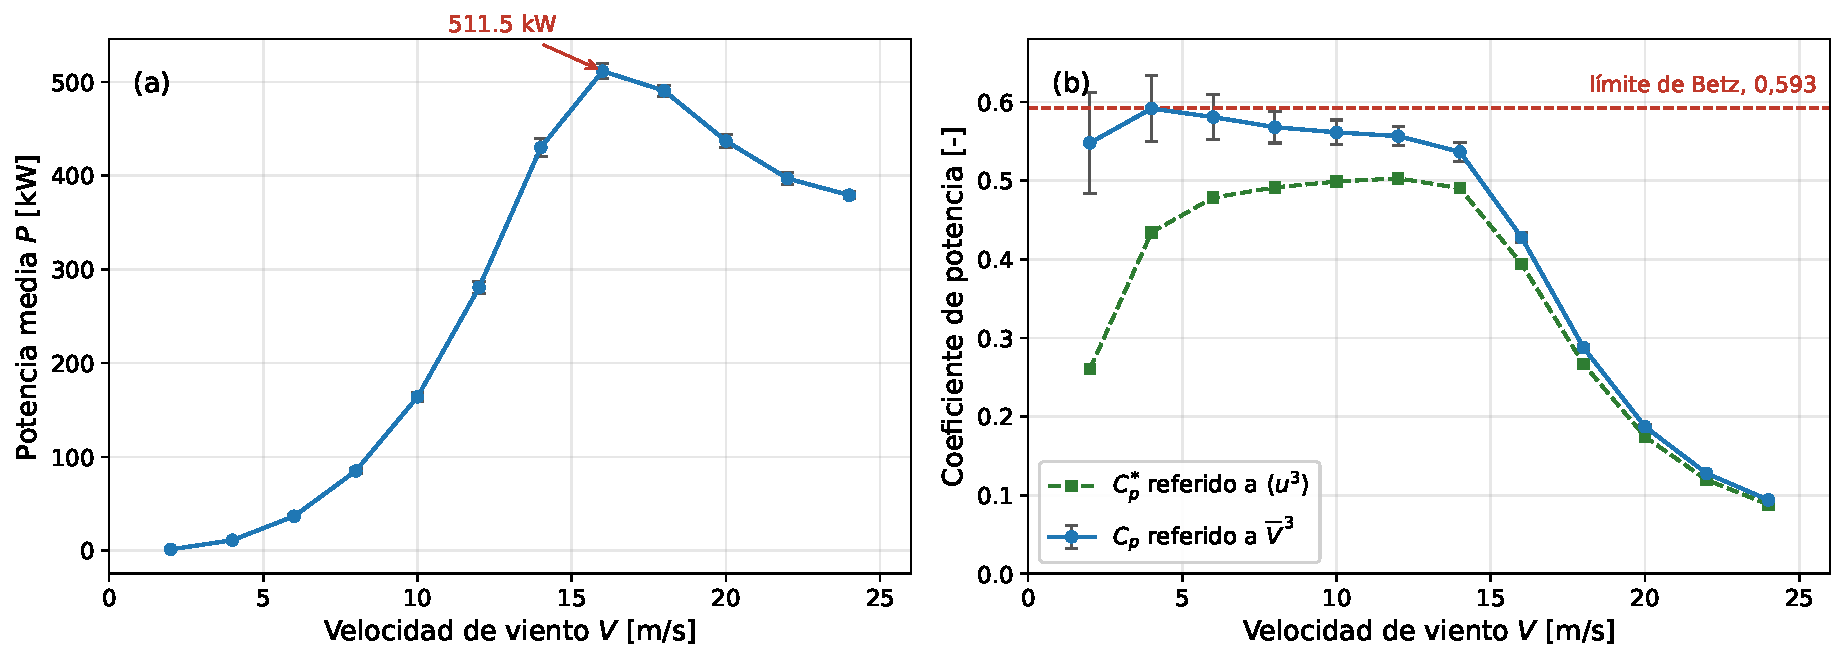
\includegraphics[width=1\textwidth]{Figuras/Figuras Resultados/curva_potencia.pdf}
    \caption{(a) Potencia media y (b) coeficiente de potencia promedio, en función de la velocidad de viento. Los puntos son el promedio de las $6$ realizaciones estocásticas simuladas por velocidad, y las barras verticales indican $\pm 1$ desviación estándar (STD) entre ellas.}
    \label{fig:curva_potencia}
\end{figure}

La barra de dispersión del primer punto de la Figura~\ref{fig:curva_potencia}b es notablemente mayor que las restantes, con una desviación estándar de $0{,}077$ en $C_p$ frente a valores entre $0{,}002$ y $0{,}020$ en el resto del rango. El origen está en la turbulencia que prescribe el NTM, ya que la desviación estándar del viento crece con la velocidad media, pero de forma menos que proporcional (Ec.~\ref{eq:ntm_sigma}), de modo que su valor relativo aumenta al bajar $V$, hasta alcanzar un $43\%$ a $2$~m/s frente a un $15\%$ a $12$~m/s. El rotor no puede seguir fluctuaciones de esa magnitud, de modo que su TSR instantáneo se dispersa con una desviación estándar de $1{,}01$ a $2$~m/s, más del triple de la que registra a $12$~m/s, y cada semilla promedia así un tramo distinto de la curva de $C_p$ frente a TSR. La dispersión no compromete las verificaciones de este capítulo, ya que la carga extrema de diseño proviene del instante registrado a $24$~m/s (Sección~\ref{sec:resultados_uls}) y el $98{,}3\%$ del daño por fatiga se concentra en las tres velocidades más altas (Sección~\ref{sec:resultados_fatiga}), de modo que la contribución de la condición de $2$~m/s a ambos estados límite es marginal.

El coeficiente de potencia de la meseta, $0{,}42$--$0{,}45$, iguala o supera el extremo superior del intervalo reportado para configuraciones H-Darrieus ($0{,}35$--$0{,}42$, Tabla~\ref{tab:tabla_vawt}) y alcanza el margen que \textcite{Essahraoui2026} atribuyen a rotores optimizados, hasta $0{,}45$. Queda así dentro de lo alcanzable por esta familia de máquinas, a diferencia del $C_{p,max} = 0{,}574$ que estima el barrido preliminar (Sección~\ref{sec:tsr_optimo}). La brecha entre ambas cifras no evidencia una inconsistencia entre métodos, sino que obedece a dos causas, una física y otra estadística. La física es la limitación del DMST ya descrita en la Sección~\ref{sec:metodos_aerodinamicos}, que las simulaciones LLFVW sí resuelven. La estadística surge de la operación bajo viento turbulento, ya que el DMST evalúa $C_{p,max}$ en un único punto estacionario, exactamente en $\lambda_{opt}$, mientras que la turbina simulada nunca permanece en ese punto.

La Figura~\ref{fig:serie_temporal_control} recorre esa segunda cadena causal para una simulación representativa a $V = 12$~m/s. La velocidad de viento incidente, panel (a), se recupera de la salida de QBlade como $V = \Omega R/\lambda$ y corresponde al campo generado por el modelo de Mann (Sección~\ref{sec:modelo_mann}); fluctúa entre $8{,}2$ y $15{,}4$~m/s en torno a una media de $11{,}7$~m/s, con una desviación estándar de $1{,}20$~m/s, un $4\%$ menor que los $1{,}25$~m/s que prescribe el NTM del emplazamiento (Sección~\ref{sec:ntm}). El panel (b) muestra que el rotor sigue esas fluctuaciones de forma suavizada, en torno a una media de $39{,}6$~rpm, ya que su inercia le impide acelerar y frenar al ritmo del viento~\parencite{Johnson2006}. El panel (c) recoge la consecuencia de ese desfase, dado que el TSR es el cociente entre ambas magnitudes y se dispersa entre $2{,}99$ y $4{,}94$ en lugar de mantenerse fijo en $\lambda_{opt}$. Para aislar el aporte del controlador, el mismo panel superpone el TSR que resultaría del mismo viento con la rotación fija en el promedio registrado ($39{,}6$~rpm). En ese escenario contrafactual la dispersión aumenta un $32\%$ (desviación estándar de $0{,}387$ frente a $0{,}292$), de modo que el controlador $K$-$\omega^2$ no solo centra el TSR en torno al óptimo, con una media de $3{,}69$ frente a $3{,}80$, sino que además reduce activamente su dispersión.

\begin{figure}[H]
    \centering
    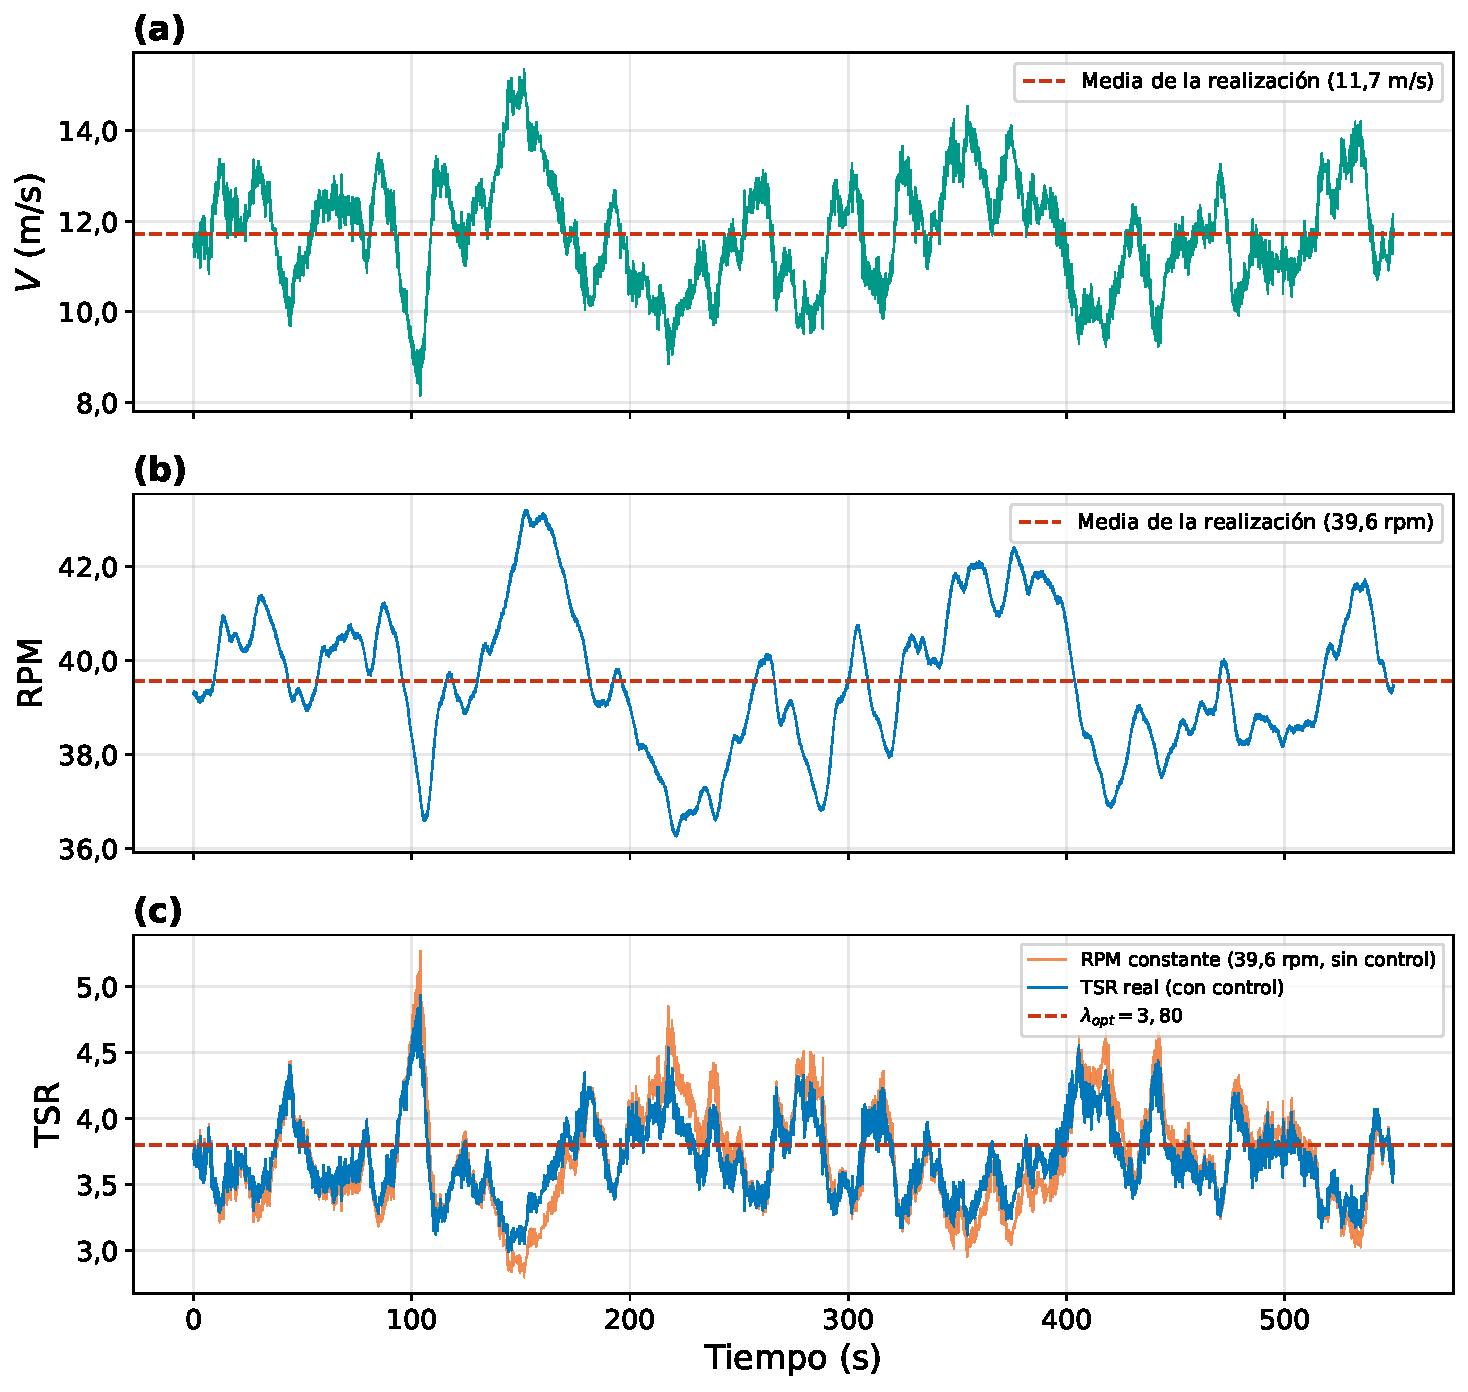
\includegraphics[width=0.95\textwidth]{Figuras/Figuras Resultados/serie_temporal_control.pdf}
    \caption[Serie temporal de viento, velocidad de rotación y TSR.]{Serie temporal de (a) velocidad de viento incidente, (b) velocidad de rotación y (c) TSR, para una simulación representativa a $V = 12$~m/s, semilla $1$. Las líneas discontinuas indican la media de la realización en (a) y (b), y $\lambda_{opt}$ en (c).}
    \label{fig:serie_temporal_control}
\end{figure}

La Tabla~\ref{tab:comparacion_adim} contrasta el rotor en estudio con las dos máquinas H-rotor de referencia de la Sección~\ref{sec:turbinas_referencia}~\parencite{Mollerstrom2019}, sobre los parámetros normalizados allí definidos. A $V = 12$~m/s la turbina del proyecto entrega $P = 201{,}5$~kW con $C_p = 0{,}432$, cifra equivalente a la potencia nominal de la T1-turbine y de la ANew-M1, ambas de $200$~kW a esa misma velocidad, y lo hace con un área de barrido intermedia entre las de ambas máquinas.

\begin{table}[H]
    \centering
    \caption[Comparación del rotor en estudio con turbinas H-rotor documentadas.]{Comparación de las dimensiones y los parámetros normalizados del rotor en estudio con turbinas H-rotor tripala documentadas y con los rangos de referencia para configuraciones H-Darrieus.}
    \label{tab:comparacion_adim}
    \begin{tabular}{lcccc}
        \hline
        \textbf{Parámetro} & \textbf{Rotor en estudio} & \textbf{T1-turbine}\textsuperscript{a} & \textbf{ANew-M1}\textsuperscript{a} & \textbf{Rango de referencia}\\
        \hline
        Diámetro $D$ (m)         & $20{,}73$ & $26{,}0$ & $24{,}0$ & ---\\
        Altura $H$ (m)           & $23{,}0$  & $24{,}0$ & $15{,}0$\textsuperscript{b} & ---\\
        Área barrida $A$ (m$^2$) & $476{,}8$ & $624$    & $360$ & ---\\
        Potencia a $12$ m/s (kW) & $201{,}5$ & $200$    & $200$ & ---\\
        $P/A$ (W/m$^2$)          & $423$     & $321$    & $556$ & $200$--$500$\textsuperscript{c}\\
        $\lambda$                & $3{,}80$  & $3{,}8$\textsuperscript{d} & --- & $2$--$5$\textsuperscript{e}\\
        $\sigma$                 & $0{,}318$ & ---      & --- & $0{,}15$--$0{,}45$\textsuperscript{e}\\
        $C_{p,max}$              & $0{,}45$  & ---      & --- & $0{,}35$--$0{,}42$\textsuperscript{e,f}\\
        \hline
        \multicolumn{5}{p{0.95\textwidth}}{\footnotesize \textsuperscript{a}Datos de \textcite{Mollerstrom2019}, Tabla~\ref{tab:hrotor_rpm}. \textsuperscript{b}Estimada como $A/D$ a partir de los datos de la fuente. \textsuperscript{c}Rango característico de un aerogenerador moderno~\parencite{Mollerstrom2019}. \textsuperscript{d}TSR objetivo documentado para la T1-turbine (Tabla~\ref{tab:t1_params})~\parencite{Mollerstrom2017,Mollerstrom2016}. \textsuperscript{e}Rango reportado para configuraciones H-Darrieus~\parencite{Essahraoui2026}, Tabla~\ref{tab:tabla_vawt}. \textsuperscript{f}La misma fuente reporta hasta $0{,}45$ para rotores optimizados.}
    \end{tabular}
\end{table}

La potencia específica del rotor en estudio se sitúa entre la de la T1-turbine y la de la ANew-M1, dentro del rango propio de un aerogenerador moderno~\parencite{Mollerstrom2019}, y su $\lambda_{opt} = 3{,}80$ coincide con el \gls{tsr} objetivo documentado para la T1-turbine~\parencite{Mollerstrom2017}. La solidez y el coeficiente de potencia caen igualmente dentro de sus rangos de referencia~\parencite{Essahraoui2026}. El dimensionamiento y el punto de operación del rotor resultan, por tanto, consistentes con los de las máquinas construidas de esta familia y escala.

El pico de $P_{max} = 503{,}4$~kW a $V = 18$~m/s corresponde a $1056$~W/m$^2$. Esta cifra no describe el dimensionamiento nominal de la máquina, sino la capacidad de sobrecarga instantánea del rotor operando fuera de su punto de diseño, y resulta del orden de los valores máximos reportados históricamente para VAWT~\parencite{Mollerstrom2019}.

La caída del coeficiente de potencia para $V > 16$~m/s es consecuencia directa de la estrategia de control, ya que al alcanzar el límite de velocidad de rotación de $42$~rpm el TSR decrece de $3{,}7$ a $1{,}8$, alejándose del $\lambda_{opt} = 3{,}80$. La pérdida es deliberada, ya que sostener el TSR óptimo a $24$~m/s exigiría girar a $84$~rpm, el doble del límite adoptado, con lo que las cargas centrífugas, proporcionales a $\Omega^2$, se cuadruplicarían. Dado que las velocidades superiores a $20$~m/s representan solo el $0{,}48\%$ de las horas del año en el emplazamiento, esto es, $42$~h/año (Sección~\ref{sec:recurso_eolico}), el costo energético de esa decisión es marginal frente al alivio estructural que proporciona.

\section{Cargas aerodinámicas para DLC 1.1}
\label{sec:resultados_uls}

Las series temporales de fuerzas obtenidas de las simulaciones anteriores constituyen la base de las verificaciones normativas que siguen. Para el DLC 1.1, los seis valores de $F_{max}$ por velocidad, el máximo de la fuerza total integrada $F_{tot}(t)$ en cada simulación (Sección~\ref{sec:anexo_f}), se ajustan a una distribución de Gumbel~\parencite{Gumbel1958}; la Tabla~\ref{tab:cargas_extremas} presenta los parámetros resultantes, junto con $F_{obs,max}$, el mayor de esos seis valores observados a cada velocidad.

\begin{table}[H]
    \centering
    \caption{Parámetros del ajuste de Gumbel para $F_{tot}$ por velocidad de viento ($N = 6$ semillas).}
    \label{tab:cargas_extremas}
    \begin{tabular}{lccc}
        \hline
        $V$ (m/s) & $\mu_j$ (kN) & $\beta_j$ (kN) & $F_{obs,max}$ (kN) \\
        \hline
        $2$  & $1{,}460$  & $0{,}15$  & $1{,}760$ \\
        $4$  & $6{,}190$  & $0{,}96$  & $9{,}230$ \\
        $6$  & $11{,}43$ & $0{,}90$  & $14{,}05$ \\
        $8$  & $19{,}66$ & $0{,}78$  & $21{,}60$ \\
        $10$ & $31{,}50$ & $1{,}36$  & $34{,}61$ \\
        $12$ & $42{,}42$ & $1{,}99$  & $47{,}06$ \\
        $14$ & $53{,}34$ & $0{,}97$  & $55{,}29$ \\
        $16$ & $63{,}10$ & $1{,}36$  & $66{,}66$ \\
        $18$ & $73{,}42$ & $1{,}91$  & $78{,}17$ \\
        $20$ & $84{,}70$ & $0{,}85$  & $86{,}04$ \\
        $22$ & $88{,}20$ & $1{,}26$  & $90{,}81$ \\
        $24$ & $100{,}8$ & $2{,}44$ & $106{,}8$ \\
        \hline
    \end{tabular}
\end{table}

Los parámetros $\mu_j$ y $\beta_j$ corresponden a la localización y escala de la distribución de Gumbel~\parencite{Gumbel1958}, estimados por el método de los momentos sobre los seis máximos observados a cada velocidad (Sección~\ref{sec:anexo_f}). Tanto $\mu_j$ como $F_{obs,max}$ crecen monótonamente con $V$, en línea con la dependencia $F \propto V^2$ de las fuerzas aerodinámicas. La Figura~\ref{fig:cargas_maximas} muestra la dispersión de estos máximos por velocidad junto con los percentiles $50\%$, $90\%$ y $99\%$ de las distribuciones ajustadas.

\begin{figure}[H]
    \centering
    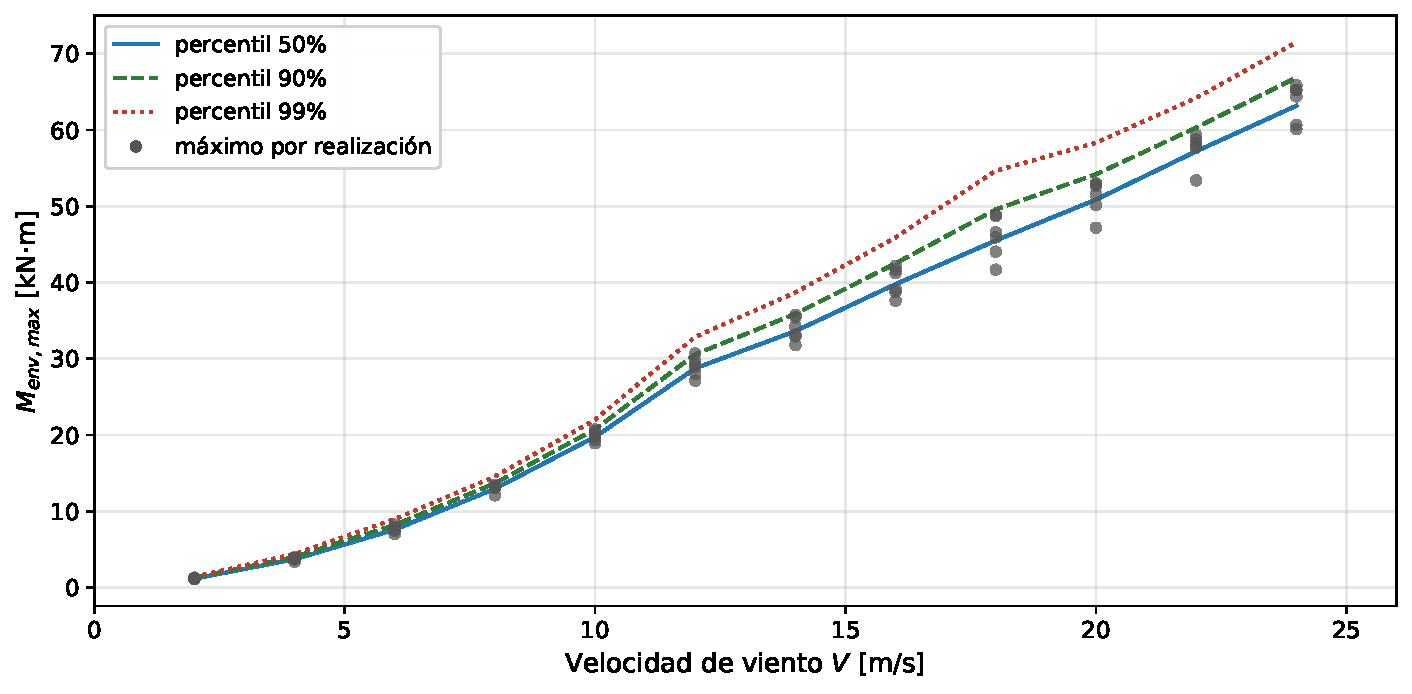
\includegraphics[width=0.9\textwidth]{Figuras/Figuras Resultados/cargas_maximas_global.pdf}
    \caption{Fuerza total máxima integrada por simulación y percentiles de Gumbel por velocidad de viento.}
    \label{fig:cargas_maximas}
\end{figure}
La dispersión de puntos para una misma velocidad refleja que, aunque las seis simulaciones comparten la misma velocidad media y la misma intensidad de turbulencia objetivo, cada una corresponde a una semilla distinta del campo de viento de Mann (Sección~\ref{sec:modelo_mann}), es decir, a una secuencia distinta de ráfagas; el $F_{max}$ que arroja cada simulación depende de la ráfaga más severa efectivamente contenida en esa realización particular, no solo de los parámetros estadísticos que todas comparten.

Esa dispersión se ensancha con la velocidad de viento, en línea con el parámetro de escala $\beta_j$ de la Tabla~\ref{tab:cargas_extremas}, que pasa de $0{,}15$~kN a $2$~m/s a $2{,}44$~kN a $24$~m/s. Como la separación entre percentiles de una distribución de Gumbel es proporcional a $\beta_j$~\parencite{Gumbel1958}, la distancia entre los percentiles $50\%$ y $99\%$ crece de $0{,}6$ a $10{,}3$~kN entre ambos extremos del rango. El crecimiento responde a dos efectos que actúan en el mismo sentido, ya que las fuerzas aerodinámicas dependen del cuadrado de la velocidad relativa (Ecs.~\ref{eq:fuerza_sustentacion} y~\ref{eq:fuerza_arrastre}) y la desviación estándar absoluta del viento que prescribe el NTM también aumenta con $V$ (Ec.~\ref{eq:ntm_sigma})~\parencite{IEC61400-1}. En términos relativos, en cambio, la dispersión se estrecha, ya que esa separación equivale al $44\%$ de $\mu_j$ a $2$~m/s y solo al $10\%$ a $24$~m/s.

El crecimiento de $\beta_j$ no es monótono, sino que oscila entre velocidades contiguas. Ello es esperable, dado que cada $\beta_j$ se estima sobre solo seis observaciones. Un remuestreo de la propia distribución ajustada, con $2 \times 10^5$ muestras de tamaño seis, sitúa el error estándar relativo del estimador por momentos de $\beta$ en un $41\%$, con el $90\%$ de las estimaciones comprendido entre $0{,}42$ y $1{,}62$ veces el valor real. La oscilación observada es, por tanto, del orden de la incertidumbre que impone el tamaño de muestra y no revela una deficiencia del ajuste. Aun así, las curvas de percentiles muestran que el modelo de Gumbel envuelve adecuadamente las observaciones, ya que las $72$ quedan por debajo del percentil $99\%$ de su velocidad. La calidad del ajuste se examina con mayor detalle en la Figura~\ref{fig:gumbel_pp}, que presenta el papel de probabilidad de Gumbel para cuatro velocidades representativas.

\begin{figure}[H]
    \centering
    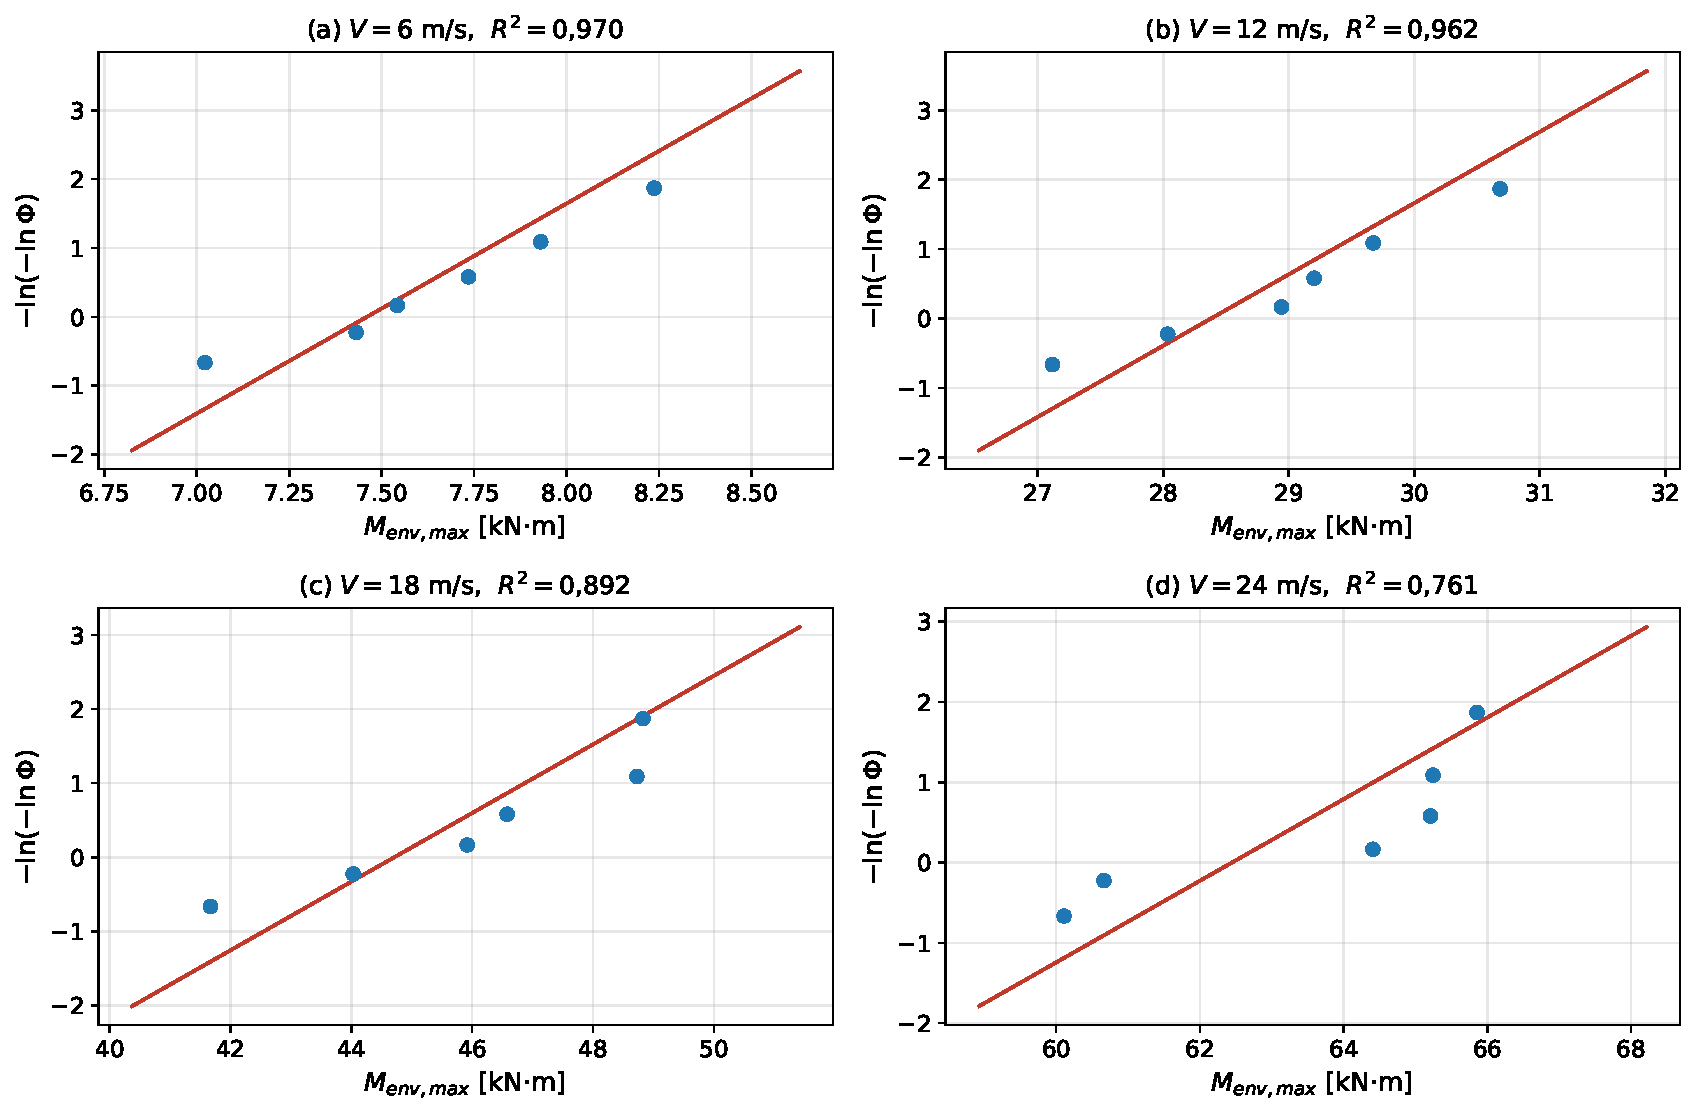
\includegraphics[width=1\textwidth]{Figuras/Figuras Resultados/gumbel_probability_paper.pdf}
    \caption{Papel de probabilidad de Gumbel para cuatro velocidades representativas. El $R^2$ de cada panel mide la linealidad de los puntos empíricos.}
    \label{fig:gumbel_pp}
\end{figure}


El papel de probabilidad es una representación en la que la distribución ajustada se convierte en una recta, de modo que la calidad del ajuste puede evaluarse a simple vista~\parencite{Gumbel1958}. Se construye aplicando a la función de distribución acumulada de Gumbel (Ec.~\ref{eq:gumbel_anexof}) la transformación $-\ln(-\ln(\Phi))$, que la reduce a $(F - \mu_j)/\beta_j$, una función lineal de la carga. El eje vertical de cada panel es esa variable reducida, y a cada uno de los seis máximos ordenados de menor a mayor se le asigna una probabilidad empírica de no excedencia $i/(n+1)$, con $i$ el orden del dato y $n = 6$. Si la distribución describe correctamente los datos, los puntos así construidos deben alinearse sobre la recta de pendiente $1/\beta_j$ que define el ajuste.

Las cuatro velocidades representativas, que cubren el rango bajo ($V = 6$~m/s), medio ($12$~m/s), alto ($18$~m/s) y extremo ($24$~m/s) del espectro operacional, presentan coeficientes de determinación $R^2$ entre $0{,}833$ y $0{,}963$, valores razonables para ajustes sobre solo seis observaciones, lo que respalda el uso de la distribución de Gumbel para modelar los máximos de $F_{tot}$.

En la Figura \ref{fig:gumbel_pp}d, se ve que tres de sus seis puntos se alinean verticalmente y se apartan de la recta. No se trata de un defecto del ajuste, sino de que esas tres semillas arrojan máximos prácticamente idénticos, comprendidos entre $100{,}459$ y $100{,}462$~kN, con una diferencia máxima de $3$~N que equivale al $0{,}003\%$ de la carga. Al compartir abscisa y diferir solo en su posición de graficado, esos tres puntos quedan forzosamente sobre una vertical, que ninguna recta puede seguir. La coincidencia proviene del régimen de operación, ya que a $24$~m/s el rotor gira en su límite de velocidad y la variación de la carga a lo largo de la revolución, idéntica en todas las semillas por depender solo de la rotación, domina sobre la contribución turbulenta que las diferencia. De ahí que el recorrido relativo de los máximos se reduzca del $29\%$ de la media a $6$~m/s a un $7\%$ a $24$~m/s, pese a que en términos absolutos la dispersión crece.

La carga característica $F_k$, correspondiente al período de retorno de $50$ años, y la carga de diseño $F_d$, que resulta de mayorarla por el factor parcial, se obtienen a partir de esta distribución mediante el procedimiento de bisección descrito en la Sección~\ref{sec:anexo_f}.

La probabilidad de excedencia objetivo de la Ec.~\ref{eq:fk_criterion}, con $T_{obs} = 600$~s y $T_{retorno} = 50$ años, resulta:

\begin{equation}
    P_e(F_k) = \frac{600\ \text{s}}{50 \times 365{,}25 \times 24 \times 3600\ \text{s}} = 3{,}8 \times 10^{-7}
    \label{eq:fk_criterion_num}
\end{equation}

La carga característica global para un período de retorno de 50 años, esto es, el valor de $F_{max}$ que satisface la Ec.~\ref{eq:fk_criterion_num}, es $F_{tot,k} = 116{,}9$~kN. La carga de diseño para el DLC 1.1 según el Anexo F de IEC 61400-1~\parencite{IEC61400-1} se obtiene aplicando el factor de seguridad parcial $\gamma_f = 1{,}25$, según la Ec.~\ref{eq:Fd_dlc11_res}:

\begin{equation}
F_{tot,d} = \gamma_f \cdot F_{tot,k} = 1{,}25 \times 116{,}9 = 146{,}1\ \text{kN}
\label{eq:Fd_dlc11_res}
\end{equation}

El instante de máxima solicitación global entre las 72 simulaciones ocurre a $V = 24$~m/s (semilla 4, $t = 188{,}3$~s), con $F_{tot} = 106{,}8$~kN; las fuerzas compañeras de ese instante se escalan por el factor $146{,}1/106{,}8 = 1{,}368$ para construir el perfil de diseño.

La distribución de esta carga a lo largo de la envergadura, esto es, las fuerzas de diseño por estación $F_{d,x}[p]$ y $F_{d,y}[p]$ para las 24 estaciones de la pala, se presenta en la Sección~\ref{sec:comparacion_dlc}, junto con la del DLC 1.3, una vez determinada la carga de este último.

\section{Cargas aerodinámicas para DLC 1.3}
\label{sec:resultados_dlc13}

Las 30 simulaciones correspondientes al DLC 1.3 (ETM, $V = 16$ a $24$~m/s) se procesan según el método de la media de máximos prescrito en la Sección 7.6.2 de la norma IEC 61400-1~\parencite{IEC61400-1}. La Tabla~\ref{tab:dlc13_maximos} presenta los máximos observados para cada una de las 6 semillas y la media por velocidad, calculados con la misma definición de $F_{tot}$ de la Ec.~\ref{eq:F_tot}.

\begin{table}[H]
    \centering
    \caption{Máximos de fuerza total integrada $F_{tot}$ por velocidad y semilla para DLC 1.3 (ETM).}
    \label{tab:dlc13_maximos}
    \begin{tabular}{lccccccc}
        \hline
        & \multicolumn{7}{c}{$F_{tot,max}$ (kN)} \\
        \cline{2-8}
        $V$ (m/s) & $S_1$ & $S_2$ & $S_3$ & $S_4$ & $S_5$ & $S_6$ & Media \\
        \hline
        $16$ & $70{,}7$ & $78{,}7$ & $69{,}9$ & $70{,}4$ & $69{,}5$ & $81{,}0$ & $73{,}4$ \\
        $18$ & $87{,}5$ & $84{,}4$ & $82{,}7$ & $77{,}6$ & $80{,}4$ & $88{,}6$ & $83{,}6$ \\
        $20$ & $88{,}8$ & $97{,}8$ & $88{,}7$ & $89{,}3$ & $91{,}1$ & $88{,}9$ & $90{,}8$ \\
        $22$ & $101{,}9$ & $101{,}8$ & $102{,}1$ & $106{,}4$ & $106{,}0$ & $102{,}0$ & $103{,}4$ \\
        $24$ & $107{,}7$ & $113{,}8$ & $113{,}0$ & $119{,}5$ & $108{,}7$ & $113{,}2$ & $\mathbf{112{,}6}$ \\
        \hline
    \end{tabular}
\end{table}

La carga característica corresponde a la mayor media entre las velocidades simuladas, $F_k = 112{,}6$~kN a $V = 24$~m/s (Destacada en la Tabla \ref{tab:dlc13_maximos}). Aplicando $\gamma_f = 1{,}35$ (Tabla 3 de la norma IEC 61400-1~\parencite{IEC61400-1}, situaciones normales sin extrapolación estadística), la carga de diseño resulta según la Ec.~\ref{eq:Fd_dlc13_res}:

\begin{equation}
    F_{d,\text{DLC 1.3}} = \gamma_f \cdot F_k = 1{,}35 \times 112{,}6 = 152{,}1\ \text{kN}
    \label{eq:Fd_dlc13_res}
\end{equation}

La Sección 7.4.1 de la norma IEC 61400-1~\parencite{IEC61400-1} vincula explícitamente ambos casos de carga, ya que permite omitir el análisis del DLC 1.1 cuando los valores extremos de diseño obtenidos del DLC 1.3 lo superan y prescribe, en caso contrario, aumentar la constante $c_{ETM}$ del modelo de turbulencia extrema hasta que el DLC 1.3 lo envuelva. Esa constante, cuyo valor por defecto de $2$~m/s fija la Sección 6.3.2.3 de la norma IEC 61400-1~\parencite{IEC61400-1}, es la adoptada en las simulaciones de este trabajo (Sección~\ref{sec:velocidades_simulacion}), sin recurrir al aumento que la norma habilita. El ETM del DLC 1.3 existe, por tanto, para sustituir la extrapolación estadística del DLC 1.1~\parencite{Galinos2015}.

Las cargas características sitúan al DLC 1.1 por encima, con $116{,}9$~kN por extrapolación estadística del NTM frente a $112{,}6$~kN por media de máximos del ETM, una diferencia del $3{,}7\%$. El orden se invierte en las cargas de diseño, $146{,}1$~kN y $152{,}1$~kN respectivamente, pero esa inversión la producen los factores parciales y no las cargas, ya que la Tabla 3 de la norma IEC 61400-1~\parencite{IEC61400-1} admite $\gamma_f = 1{,}25$ para el DLC 1.1 por determinarse mediante extrapolación estadística, frente al $\gamma_f = 1{,}35$ del DLC 1.3.

\textcite{Galinos2015} obtiene el mismo ordenamiento de las cargas características en un rotor Darrieus de $5$~MW, donde los valores extrapolados del DLC 1.1 superan a los del DLC 1.3 incluso al elevar $c_{ETM}$ a $3$~m/s. La explicación que propone es que las cargas de una VAWT están dominadas por la fluctuación determinista a frecuencia $1P$, esto es, la que se repite una vez por cada revolución del rotor, ya que cada pala recorre en cada vuelta un ciclo completo de ángulo de ataque (Sección~\ref{sec:aerodinamica}). Esa componente no depende de la turbulencia, por lo que las cargas de una VAWT resultan menos sensibles a ella que las de una HAWT, de modo que el ETM, que actúa amplificando precisamente la componente turbulenta, eleva la carga de una VAWT menos de lo que la elevaría en la máquina de eje horizontal sobre la que fue calibrado. Esa dominancia determinista se observa igualmente en las simulaciones de este trabajo, ya que a $24$~m/s tres de las seis semillas del DLC 1.1 arrojan máximos que coinciden dentro del $0{,}003\%$ (Sección~\ref{sec:resultados_uls}). El propio autor advierte, no obstante, que su conclusión proviene del análisis de un único rotor Darrieus y que debe verificarse sobre otros modelos antes de proponer cambios a la norma.

El criterio que la Sección 7.4.1 de la norma IEC 61400-1~\parencite{IEC61400-1} define para esa omisión se evalúa sobre los momentos flectores en la raíz de la pala y la deflexión de punta, no sobre la carga global. Como se verá en la Sección~\ref{sec:resultados_fem}, los resultados del modelo estructural muestran que el DLC 1.3 no supera al DLC 1.1 en ninguna de las dos magnitudes con que aquí se verifica la pala, con una deflexión de $0{,}164$~m frente a $0{,}169$~m y una tensión principal máxima de $156{,}8$~MPa frente a $163{,}4$~MPa. El análisis del DLC 1.1 no puede omitirse y ambos casos se conservan en la verificación.

Que el DLC 1.1 gobierne pese a su menor carga de diseño responde a la forma de los perfiles de carga. El del DLC 1.1 proviene de un único instante de la simulación y concentra la solicitación en el vano central, mientras que el del DLC 1.3, construido como media de máximos por estación, resulta espacialmente más suave (Sección~\ref{sec:comparacion_dlc}).

\section{Comparación de fuerzas por estación entre DLC}
\label{sec:comparacion_dlc}

Definidas las cargas globales de ambos casos últimos, resta distribuirlas a lo largo de la pala para su aplicación en el modelo estructural. La Figura~\ref{fig:comparacion_fuerzas_dlc} presenta el perfil de fuerzas de diseño $F_d$ a lo largo de la envergadura para ambos casos, construido en cada uno según el procedimiento que le corresponde, con escalamiento uniforme de las fuerzas compañeras del instante de máxima solicitación global en el DLC 1.1 (Sección~\ref{sec:anexo_f}), y media por estación de los perfiles de las seis semillas a la velocidad gobernante en el DLC 1.3 (Sección~\ref{sec:anexo_dlc13}).

\begin{figure}[H]
    \centering
    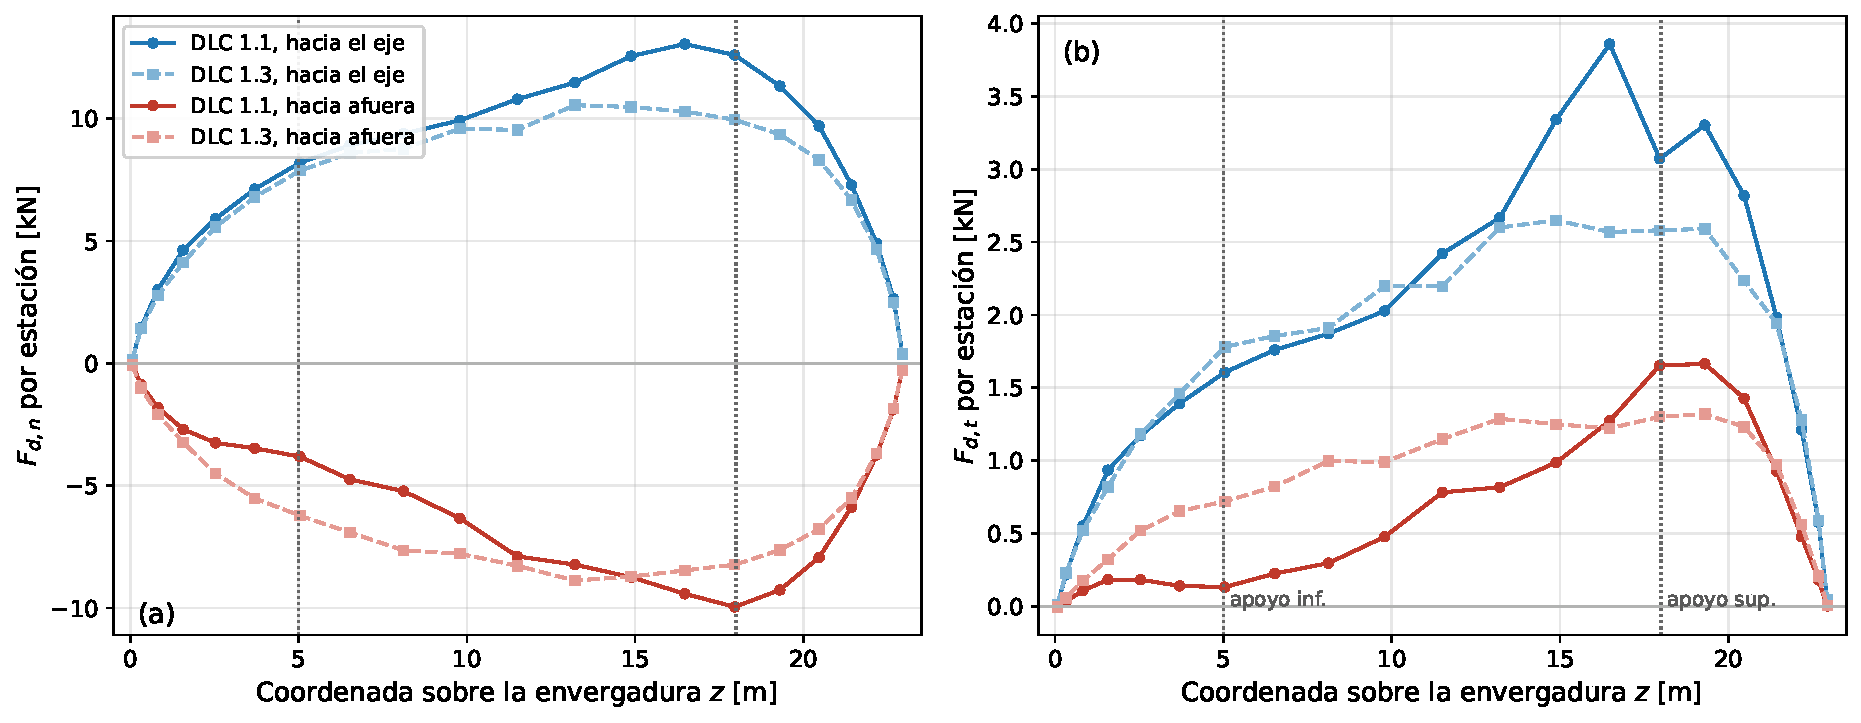
\includegraphics[width=1\textwidth]{Figuras/Figuras Resultados/comparacion_fuerzas_dlc.pdf}
    \caption{Comparación de fuerzas de diseño por estación entre DLC 1.1 (NTM) y DLC 1.3 (ETM): (a) componente normal a la cuerda $F_{d,x}$ y (b) componente en el sentido de la cuerda $F_{d,y}$, según los ejes locales de la Figura~\ref{fig:ejes_locales}. El eje vertical del panel (b) está invertido, ya que $F_{d,y}$ es negativa en todas las estaciones.}
    \label{fig:comparacion_fuerzas_dlc}
\end{figure}

Cada panel de la Figura~\ref{fig:comparacion_fuerzas_dlc} recorre la envergadura desde la raíz ($z = 0$) hasta la punta ($z = 23$~m) y compara, estación por estación, la fuerza de diseño de ambos casos en una de las dos direcciones del sistema local de la pala (Figura~\ref{fig:ejes_locales}). El panel (a) corresponde a la componente normal a la cuerda, $F_{d,x}$, y el (b) a la componente en el sentido de la cuerda, $F_{d,y}$. Las líneas verticales punteadas marcan las dos conexiones con los brazos, en $z = 5$ y $z = 17$~m, que separan los dos tramos en voladizo del vano central.

Ambos paneles conservan el signo de la fuerza. En el instante de diseño, $F_{d,x}$ es positiva y $F_{d,y}$ negativa en las 24 estaciones de los dos casos, lo que significa que la componente normal apunta hacia el extradós y la tangencial hacia el borde de ataque, según la orientación de los ejes $X_l$ e $Y_l$ de la Figura~\ref{fig:ejes_locales}. El eje vertical del panel (b) se representa invertido para que, mostrando los valores negativos que corresponden, la curva no quede dibujada hacia abajo. La componente normal domina el estado de carga, ya que su cociente con la tangencial, $|F_{d,x}/F_{d,y}|$, se mantiene entre $2{,}8$ y $3{,}0$ a lo largo de todo el vano central en ambos casos, y solo crece en las dos estaciones extremas, donde ambas componentes son pequeñas y su cociente pierde significado. Ese predominio es el esperable en un perfil con flujo adherido, donde la sustentación, perpendicular a la cuerda, supera con holgura a la fuerza en el sentido de la cuerda.

Las dos distribuciones concentran la carga en la región media de la pala y decaen hacia la raíz y la punta, pero difieren en la forma de ese decaimiento. El perfil del DLC 1.1 tiene un máximo definido en $z \approx 10$--$11$~m y desde ahí disminuye de forma progresiva, mientras que el del DLC 1.3 se mantiene casi plano a lo largo del vano central y de los tramos contiguos. En la componente tangencial, entre $z = 5$ y $z = 18$~m el perfil del DLC 1.3 varía un $3\%$ frente al $19\%$ del DLC 1.1, y entre su máximo y $z = 20$~m el DLC 1.1 pierde un $27\%$ frente al $6\%$ del DLC 1.3. La caída abrupta del DLC 1.3 se concentra en la última estación, donde pierde un $79\%$. La diferencia proviene de cómo se construye cada perfil. El del DLC 1.1 es un único instante de una única realización, de modo que conserva la distribución espacial que la simulación entrega en ese momento, con su máximo en una posición concreta. El del DLC 1.3 promedia estación por estación los perfiles compañeros de las seis semillas, cada uno tomado en el instante de máxima solicitación de su propia realización (Sección~\ref{sec:anexo_dlc13}); como esos seis instantes corresponden a azimuts y campos de viento distintos, el promedio atenúa los rasgos propios de cada uno y entrega una distribución más uniforme. El resultado es que las fuerzas del DLC 1.3 superan a las del DLC 1.1 en los tramos en voladizo, mientras que en el vano central entre brazos ambas componentes del DLC 1.1 resultan mayores, diferencia que tiene consecuencias directas sobre la respuesta estructural, como se verá en la Sección~\ref{sec:resultados_fem}.

La caída de la carga hacia los dos extremos responde a las pérdidas de punta, ya que los vórtices desprendidos en los extremos libres de la pala inducen velocidades que reducen el ángulo de ataque efectivo, y con ello la sustentación, en esas regiones~\parencite{Anderson2016}, efecto que el método LLFVW resuelve implícitamente (Sección~\ref{sec:metodos_aerodinamicos})~\parencite{marten2019qblade}.

La tabla completa de fuerzas $F_{d,x}$ y $F_{d,y}$ para las 24 estaciones, expresadas como resultantes por segmento, se presenta en el \hyperref[anexo:fuerzas]{Anexo~A} para su ingreso directo al modelo de elementos finitos en Ansys, construida según los procedimientos de las Secciones~\ref{sec:anexo_f} y~\ref{sec:anexo_dlc13}.

\section{Evaluación de fatiga (DLC 1.2)}
\label{sec:resultados_fatiga}

La verificación a fatiga del DLC 1.2 se presenta siguiendo la cadena de cálculo: el procesamiento de las series de carga en ciclos de tensión y su escalamiento a un año de operación; el contraste de la demanda así obtenida con la curva S-N del material; la distribución del daño anual entre las velocidades del rango operacional; y el daño acumulado sobre la vida útil de diseño.

\subsection{Procesamiento de las series de carga}

Las 72 series temporales del DLC 1.2 se procesan mediante el momento flector $M_{res}(t)$ en la sección crítica $z_{crit} = 5$~m (conexión con el brazo inferior, donde el FEM localiza la tensión máxima) y el factor de proporcionalidad $K_{aero} = 0{,}752$~MPa/(kN$\cdot$m), conforme a la metodología descrita en la Sección~\ref{sec:anexo_g}. Dicho factor resulta de las dos corridas FEM de la Sección~\ref{sec:resultados_fem}, como la tensión bajo la carga de diseño completa, $\sigma_{1,\max} = 163{,}4$~MPa, menos la que producen las cargas inerciales por sí solas, $\sigma_{in} = 114{,}5$~MPa, dividida por el momento de diseño de $65{,}0$~kN$\cdot$m. Esta última tensión se reincorpora después como el nivel medio sobre el que oscila la historia de tensión. Sobre esa historia se aplica el conteo de ciclos Rainflow~\parencite{ASTM_E1049,Matsuishi1968} y la corrección por tensión media según el diagrama de Goodman, conforme exige la Sección 7.6.3 de la norma IEC 61400-1~\parencite{IEC61400-1}. Dado que cada simulación cubre únicamente $T_{sim} = 550$~s, los ciclos contabilizados a cada velocidad deben expandirse al tiempo que el viento permanece en ese intervalo a lo largo de un año. La Tabla~\ref{tab:weibull_fatiga} presenta los parámetros de dicho escalamiento temporal para las doce velocidades del rango operacional. Una serie temporal representativa del procesamiento Rainflow para $V = 10$~m/s se presenta en el \hyperref[anexo:fuerzas]{Anexo~A}.

En la Tabla~\ref{tab:weibull_fatiga}, $f_W(V)$ es la densidad de probabilidad de Weibull, $t_j$ el tiempo anual que el viento permanece en cada intervalo de velocidad y $t_j/T_{sim}$ el número de simulaciones equivalentes por año.

\begin{table}[H]
    \centering
    \caption{Parámetros de escalamiento temporal según la distribución de Weibull del emplazamiento.}
    \label{tab:weibull_fatiga}
    \begin{tabular}{lccccc}
        \hline
        $V$ (m/s) & $f_W(V)$ & Prob. (\%) & $t_j$ (h/año) & $t_j$ (s/año) & $t_j/T_{sim}$ \\
        \hline
        $2$  & $0{,}0431$ & $8{,}62$ & $761{,}9$  & $2{,}74 \times 10^6$ & $4\,986$ \\
        $4$  & $0{,}0794$ & $15{,}89$ & $1\,407{,}9$ & $5{,}07 \times 10^6$ & $9\,216$ \\
        $6$  & $0{,}0967$ & $19{,}34$ & $1\,711{,}7$ & $6{,}16 \times 10^6$ & $11\,204$ \\
        $8$  & $0{,}0930$ & $18{,}59$ & $1\,641{,}0$ & $5{,}91 \times 10^6$ & $10\,741$ \\
        $10$ & $0{,}0746$ & $14{,}91$ & $1\,310{,}9$ & $4{,}72 \times 10^6$ & $8\,581$ \\
        $12$ & $0{,}0511$ & $10{,}22$ & $893{,}5$  & $3{,}22 \times 10^6$ & $5\,848$ \\
        $14$ & $0{,}0303$ & $6{,}05$  & $525{,}7$  & $1{,}89 \times 10^6$ & $3\,441$ \\
        $16$ & $0{,}0156$ & $3{,}12$  & $268{,}8$  & $9{,}68 \times 10^5$ & $1\,760$ \\
        $18$ & $0{,}0070$ & $1{,}40$  & $119{,}9$  & $4{,}32 \times 10^5$ & $785$ \\
        $20$ & $0{,}0027$ & $0{,}55$  & $46{,}8$   & $1{,}68 \times 10^5$ & $306$ \\
        $22$ & $0{,}0009$ & $0{,}19$  & $16{,}0$   & $5{,}76 \times 10^4$ & $105$ \\
        $24$ & $0{,}0003$ & $0{,}06$  & $4{,}8$    & $1{,}72 \times 10^4$ & $31$ \\
        \hline
    \end{tabular}
\end{table}

El factor $t_j/T_{sim}$ cuantifica cuántas veces debe repetirse el espectro de ciclos de cada simulación para representar un año de operación. Su distribución sigue directamente a la de Weibull del emplazamiento, ya que alcanza su máximo en las velocidades intermedias ($V = 6$--$8$~m/s), las más frecuentes, y cae más de dos órdenes de magnitud hacia el extremo superior del rango, donde el viento sopla solo unas pocas horas al año. Aplicado este escalamiento, el espectro de ciclos de cada simulación queda expresado sobre un año de operación y puede contrastarse con la resistencia del material.

\subsection{Curva S-N y espectro de fatiga}

La Figura~\ref{fig:curva_sn_gfrp} presenta la curva S-N del GFRP en sus formas nominal y factoreada ($\gamma_m = 1{,}7$, $\gamma_n = 1{,}15$ según la Sección 7.6.3 de la norma IEC 61400-1~\parencite{IEC61400-1}), junto con el espectro colectivo anual que resulta del escalamiento anterior. En la ecuación de Basquin~\parencite{Basquin1910}, la resistencia última $\sigma_u = 242{,}1$~MPa corresponde al valor proporcionado por el fabricante de la pala (Tabla~\ref{tab:material_pala}), mientras que el exponente de fatiga $b = -0{,}045$ proviene de \textcite{Huh2012} para un tejido bidireccional ($\pm 45^\circ$) fabricado por infusión al vacío.

\begin{figure}[H]
    \centering
    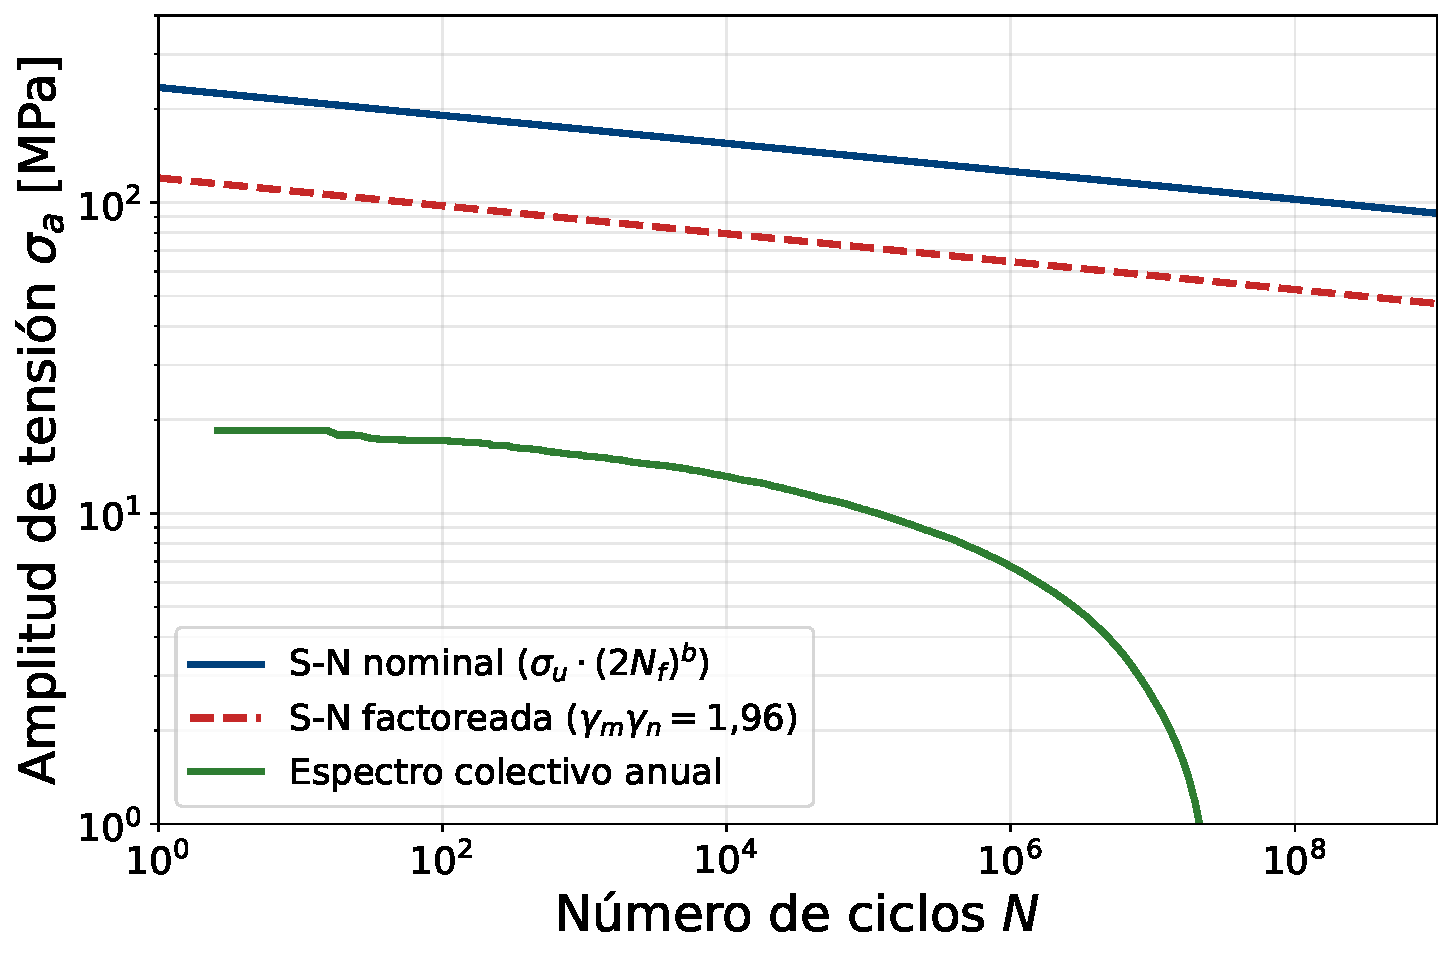
\includegraphics[width=0.95\textwidth]{Figuras/Figuras Resultados/curva_sn_gfrp.pdf}
    \caption{Curva S-N del GFRP $\pm 45^\circ$ en su forma nominal y factoreada, y espectro colectivo anual de fatiga.}
    \label{fig:curva_sn_gfrp}
\end{figure}

La superposición de ambas curvas en un mismo gráfico permite apreciar directamente el margen de seguridad a fatiga, ya que el espectro colectivo se sitúa por debajo de la curva S-N factoreada en todo el rango de ciclos. Las mayores amplitudes del espectro, que no superan los $18{,}4$~MPa, corresponden a las velocidades de viento más altas y a un número reducido de ciclos anuales, mientras que la gran mayoría de los ciclos se concentra en amplitudes de pocos MPa. Esas amplitudes se superponen a una tensión media elevada, comprendida entre $114{,}5$ y $135{,}4$~MPa, que impone la carga permanente de rotación y que sitúa los ciclos en régimen de tracción-tracción, con una razón de tensiones media de $R \approx 0{,}88$.

\subsection{Daño acumulado por velocidad de viento}

El daño de cada ciclo se obtiene al confrontar su amplitud con la curva S-N, y su contribución anual, al ponderarlo por el escalamiento temporal de la Tabla~\ref{tab:weibull_fatiga}. La Figura~\ref{fig:daño_por_viento} presenta el reparto resultante entre las doce velocidades del rango operacional.

\begin{figure}[H]
    \centering
    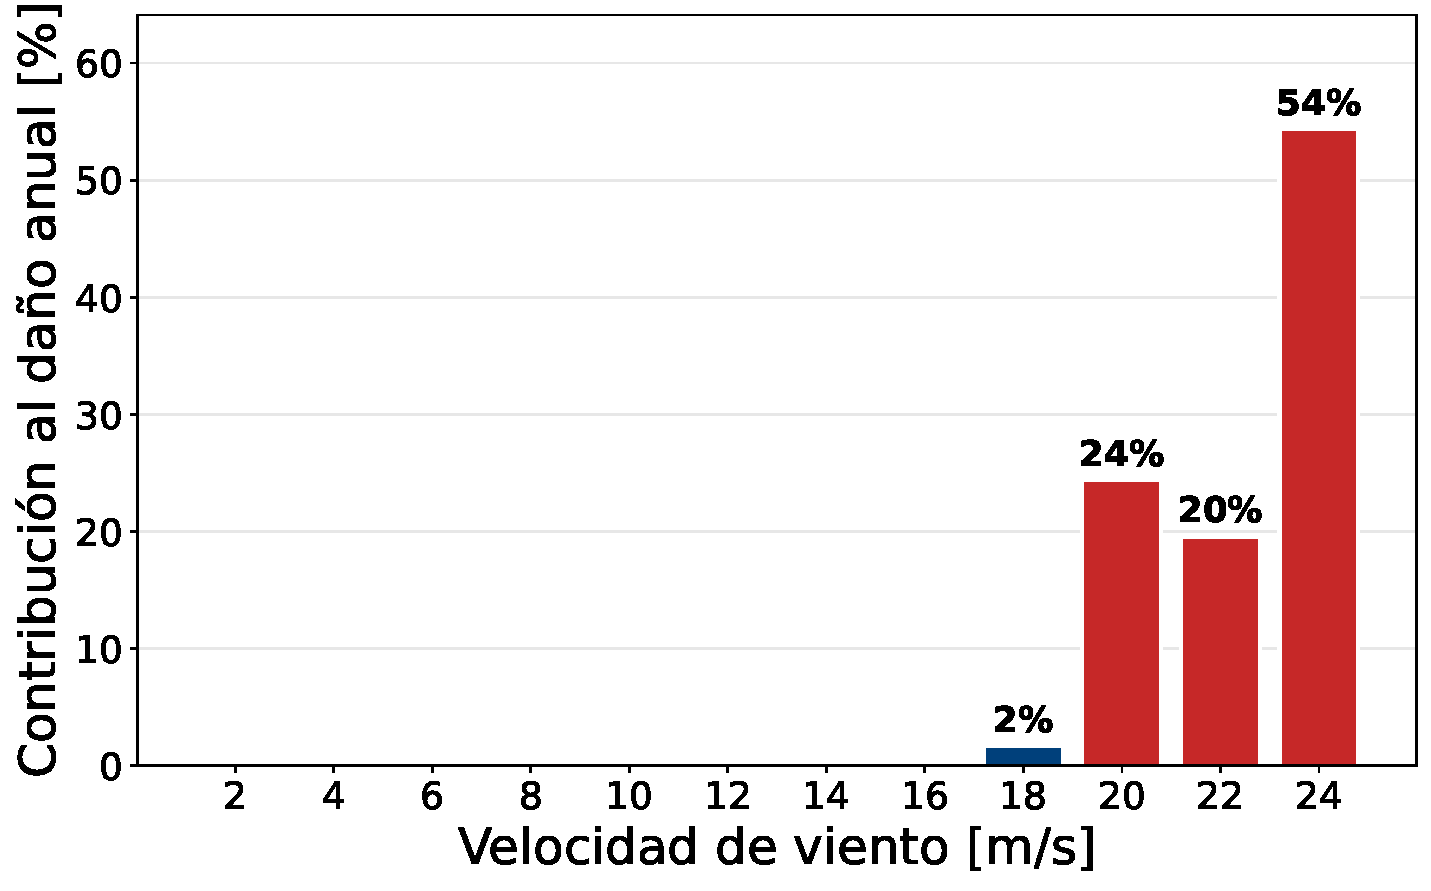
\includegraphics[width=0.7\textwidth]{Figuras/Figuras Resultados/daño_por_viento.pdf}
    \caption{Contribución porcentual de cada velocidad de viento al daño anual por fatiga.}
    \label{fig:daño_por_viento}
\end{figure}

El $98{,}3\%$ del daño se concentra en las tres velocidades más altas ($V = 20$--$24$~m/s) que, sin embargo, ocurren apenas el $0{,}8\%$ del año ($68$~h/año). El resultado es opuesto al que sugiere el factor de escalamiento y es característico de la fatiga en aerogeneradores~\parencite{Brondsted2005}, ya que la relación no lineal entre amplitud de tensión y daño ($D \propto \sigma_a^{|1/b|} = \sigma_a^{22{,}2}$) hace que los ciclos de mayor amplitud, aunque poco frecuentes, dominen el daño acumulado por sobre la frecuencia de ocurrencia.

\subsection{Daño acumulado total}

Sumando las contribuciones de las doce velocidades, el daño anual acumulado según la regla de Palmgren-Miner~\parencite{Miner1945} es $D_{\text{año}} = 3{,}22 \times 10^{-9}$. Para la vida útil de diseño de $20$ años, el daño total asciende al valor de la Ec.~\ref{eq:D20_res}:

\begin{equation}
    D_{20} = 20 \cdot D_{\text{año}} = 6{,}45 \times 10^{-8}
    \label{eq:D20_res}
\end{equation}

Este valor, muy por debajo del límite normativo de la Ec.~\ref{eq:fatiga_criterio}, indica que la fatiga no es un mecanismo dimensionante para la pala bajo las condiciones analizadas. La solicitación a fatiga se mantiene acotada por la combinación de dos factores. Primero, como muestra el espectro de la Figura~\ref{fig:curva_sn_gfrp}, las amplitudes de tensión no superan los $18{,}4$~MPa, en torno a un $8\%$ de $\sigma_u = 242{,}1$~MPa, ni siquiera en las condiciones más exigentes. Segundo, el exponente de Basquin $b = -0{,}045$, típico de tejidos biaxiales $\pm 45^\circ$ fabricados por infusión al vacío~\parencite{Huh2012}, produce una curva S-N excepcionalmente plana, cuya resistencia a fatiga decae muy lentamente con el número de ciclos, por lo que se requieren amplitudes de tensión cercanas a la resistencia última para generar daño significativo.

Conviene acotar el alcance de esa cifra. Un daño de $6{,}45 \times 10^{-8}$ proviene de extrapolar la curva de Basquin muy por encima del rango de ciclos ensayado por \textcite{Huh2012}, de modo que su magnitud exacta no admite lectura literal como predicción de vida. La verificación admite, en cambio, una cota que no depende de esa extrapolación. El ciclo más severo de toda la campaña, de amplitud $18{,}4$~MPa sobre una media de $135{,}4$~MPa, corregido por Goodman y factorado, equivale a una amplitud de diseño de $81{,}8$~MPa, a la que la curva S-N asigna $N_f = 1{,}49 \times 10^{10}$ ciclos. El rotor completa $4{,}42 \times 10^{8}$ revoluciones en los $20$ años de vida de diseño girando a su velocidad máxima, de modo que aun bajo el supuesto extremo de que todos esos ciclos fueran el más severo registrado, el daño acumulado alcanzaría $D_{20} = 0{,}030$, todavía por debajo de la unidad. La verificación a fatiga se satisface, por tanto, con independencia del tramo extrapolado de la curva.

El margen a fatiga no habilita, sin embargo, una reducción del espesor de pared, ya que, como se verá en la Sección~\ref{sec:resultados_fem}, la verificación de estabilidad demanda rigidización adicional de la piel, no menos material. La fatiga queda así descartada como criterio dimensionante, y el diseño pasa a estar gobernado por la estabilidad y, en segundo término, por la resistencia última.

\section{Verificación estructural de la pala}
\label{sec:resultados_fem}

Las fuerzas de diseño por estación de la Sección~\ref{sec:comparacion_dlc}, junto con la aceleración centrífuga, constituyen las cargas del modelo de elementos finitos descrito en la Sección~\ref{sec:fem}. Su resolución se aborda en tres pasos: primero se verifica que los resultados sean independientes de la discretización, luego se describen las condiciones de borde y cargas aplicadas, y finalmente se presentan las tensiones y deformaciones de los DLC 1.1 y 1.3, con las que se evalúan los criterios de resistencia última, estabilidad y deflexión de la norma IEC 61400-1~\parencite{IEC61400-1}.

\subsection{Convergencia de malla}

La independencia de los resultados respecto del tamaño de elemento se verifica mediante un análisis de convergencia con cinco tamaños de elemento, desde $20$~mm hasta $12$~mm de tamaño característico, sobre el caso DLC 1.1. La Figura~\ref{fig:convergencia_malla} presenta la evolución de la tensión principal máxima en función del tamaño de elemento y la Tabla~\ref{tab:convergencia_malla} resume los valores obtenidos y la variación porcentual entre mallas consecutivas.

\begin{figure}[H]
    \centering
    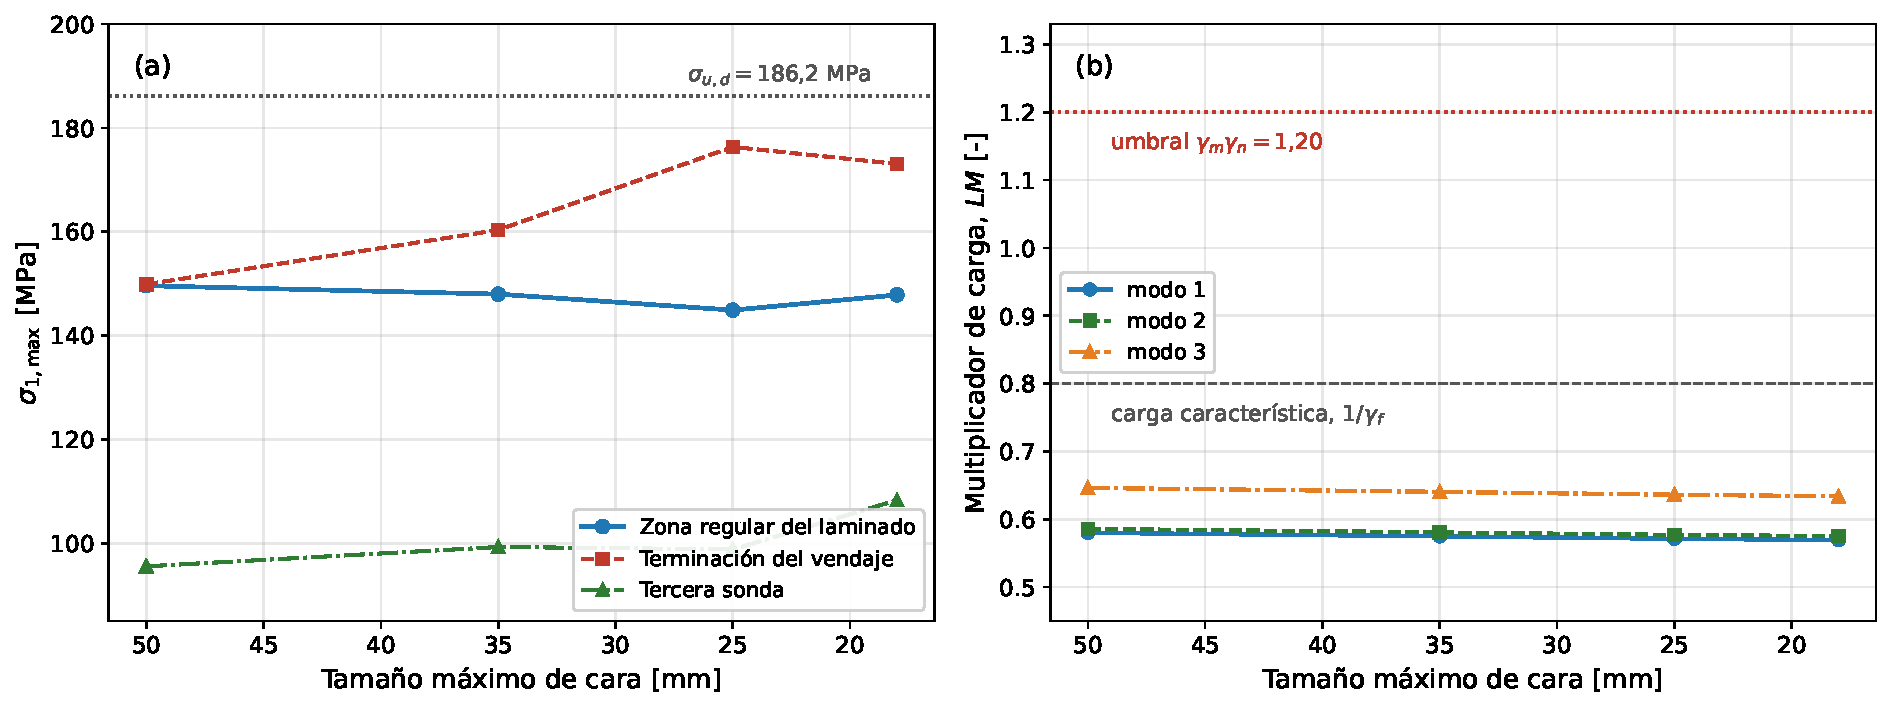
\includegraphics[width=0.65\textwidth]{Figuras/Figuras Resultados/convergencia_malla.pdf}
    \caption{Convergencia de malla, tensión principal máxima $\sigma_{1,\text{max}}$ en función del tamaño característico de elemento.}
    \label{fig:convergencia_malla}
\end{figure}

\begin{table}[H]
    \centering
    \caption{Análisis de convergencia de malla para cinco tamaños de elemento.}
    \label{tab:convergencia_malla}
    \begin{tabular}{lcccccc}
        \hline
        \textbf{Tamaño (mm)} & $\sigma_{1,\max}$ \textbf{(MPa)} & $\Delta\sigma_1$ \textbf{(\%)} & $\sigma_{3,\min}$ \textbf{(MPa)} & $\Delta\sigma_3$ \textbf{(\%)} & $\mathbf{F_{s1}}$ \textbf{(kN)} & $\mathbf{F_{s2}}$ \textbf{(kN)} \\
        \hline
        $20$ & $151{,}6$ & ---      & $-121{,}7$ & ---      & $153{,}26$ & $151{,}55$ \\
        $18$ & $153{,}8$ & $1{,}45$ & $-122{,}6$ & $0{,}69$ & $153{,}29$ & $151{,}58$ \\
        $16$ & $159{,}5$ & $3{,}66$ & $-124{,}5$ & $1{,}55$ & $153{,}31$ & $151{,}60$ \\
        $14$ & $162{,}2$ & $1{,}70$ & $-125{,}5$ & $0{,}87$ & $153{,}31$ & $151{,}60$ \\
        $12$ & $163{,}4$ & $0{,}76$ & $-127{,}1$ & $1{,}21$ & $153{,}31$ & $151{,}60$ \\
        \hline
    \end{tabular}
\end{table}

La diferencia en la tensión principal máxima entre las dos mallas más finas ($14$~mm y $12$~mm) es del $0{,}76\%$, muy por debajo del criterio del $5\%$ adoptado en este trabajo (Sección~\ref{sec:fem}). Este margen holgado respecto al umbral de la literatura~\parencite{Qin2026,Hameed2015,Boudounit2020} indica que la malla de $12$~mm resuelve adecuadamente los gradientes de tensión en la zona de interés, particularmente en las conexiones strut--pala donde se concentran las máximas solicitaciones. Las fuerzas de reacción en ambos struts presentan variaciones inferiores al $0{,}04\%$ en todas las mallas, confirmando que el equilibrio global de fuerzas es independiente de la discretización. Se selecciona el tamaño de elemento de $12$~mm para las simulaciones definitivas.

La malla definitiva presenta una calidad de elemento media (\textit{element quality}) de $0{,}9893$. Esta métrica de Ansys toma el valor $1$ para un elemento de forma ideal, por lo que el valor obtenido indica que la práctica totalidad de los elementos conserva una geometría próxima a la óptima, sin zonas de distorsión que pudieran degradar localmente la solución.

\subsection{Modelo de elementos finitos}

La Figura~\ref{fig:fem_cb} muestra el modelo con las condiciones de borde que define la Sección~\ref{sec:condiciones_borde}, esto es, los empotramientos en las dos conexiones con los brazos y la aceleración centrífuga aplicada radialmente sobre todos los elementos de la pala.

\begin{figure}[H]
    \centering
    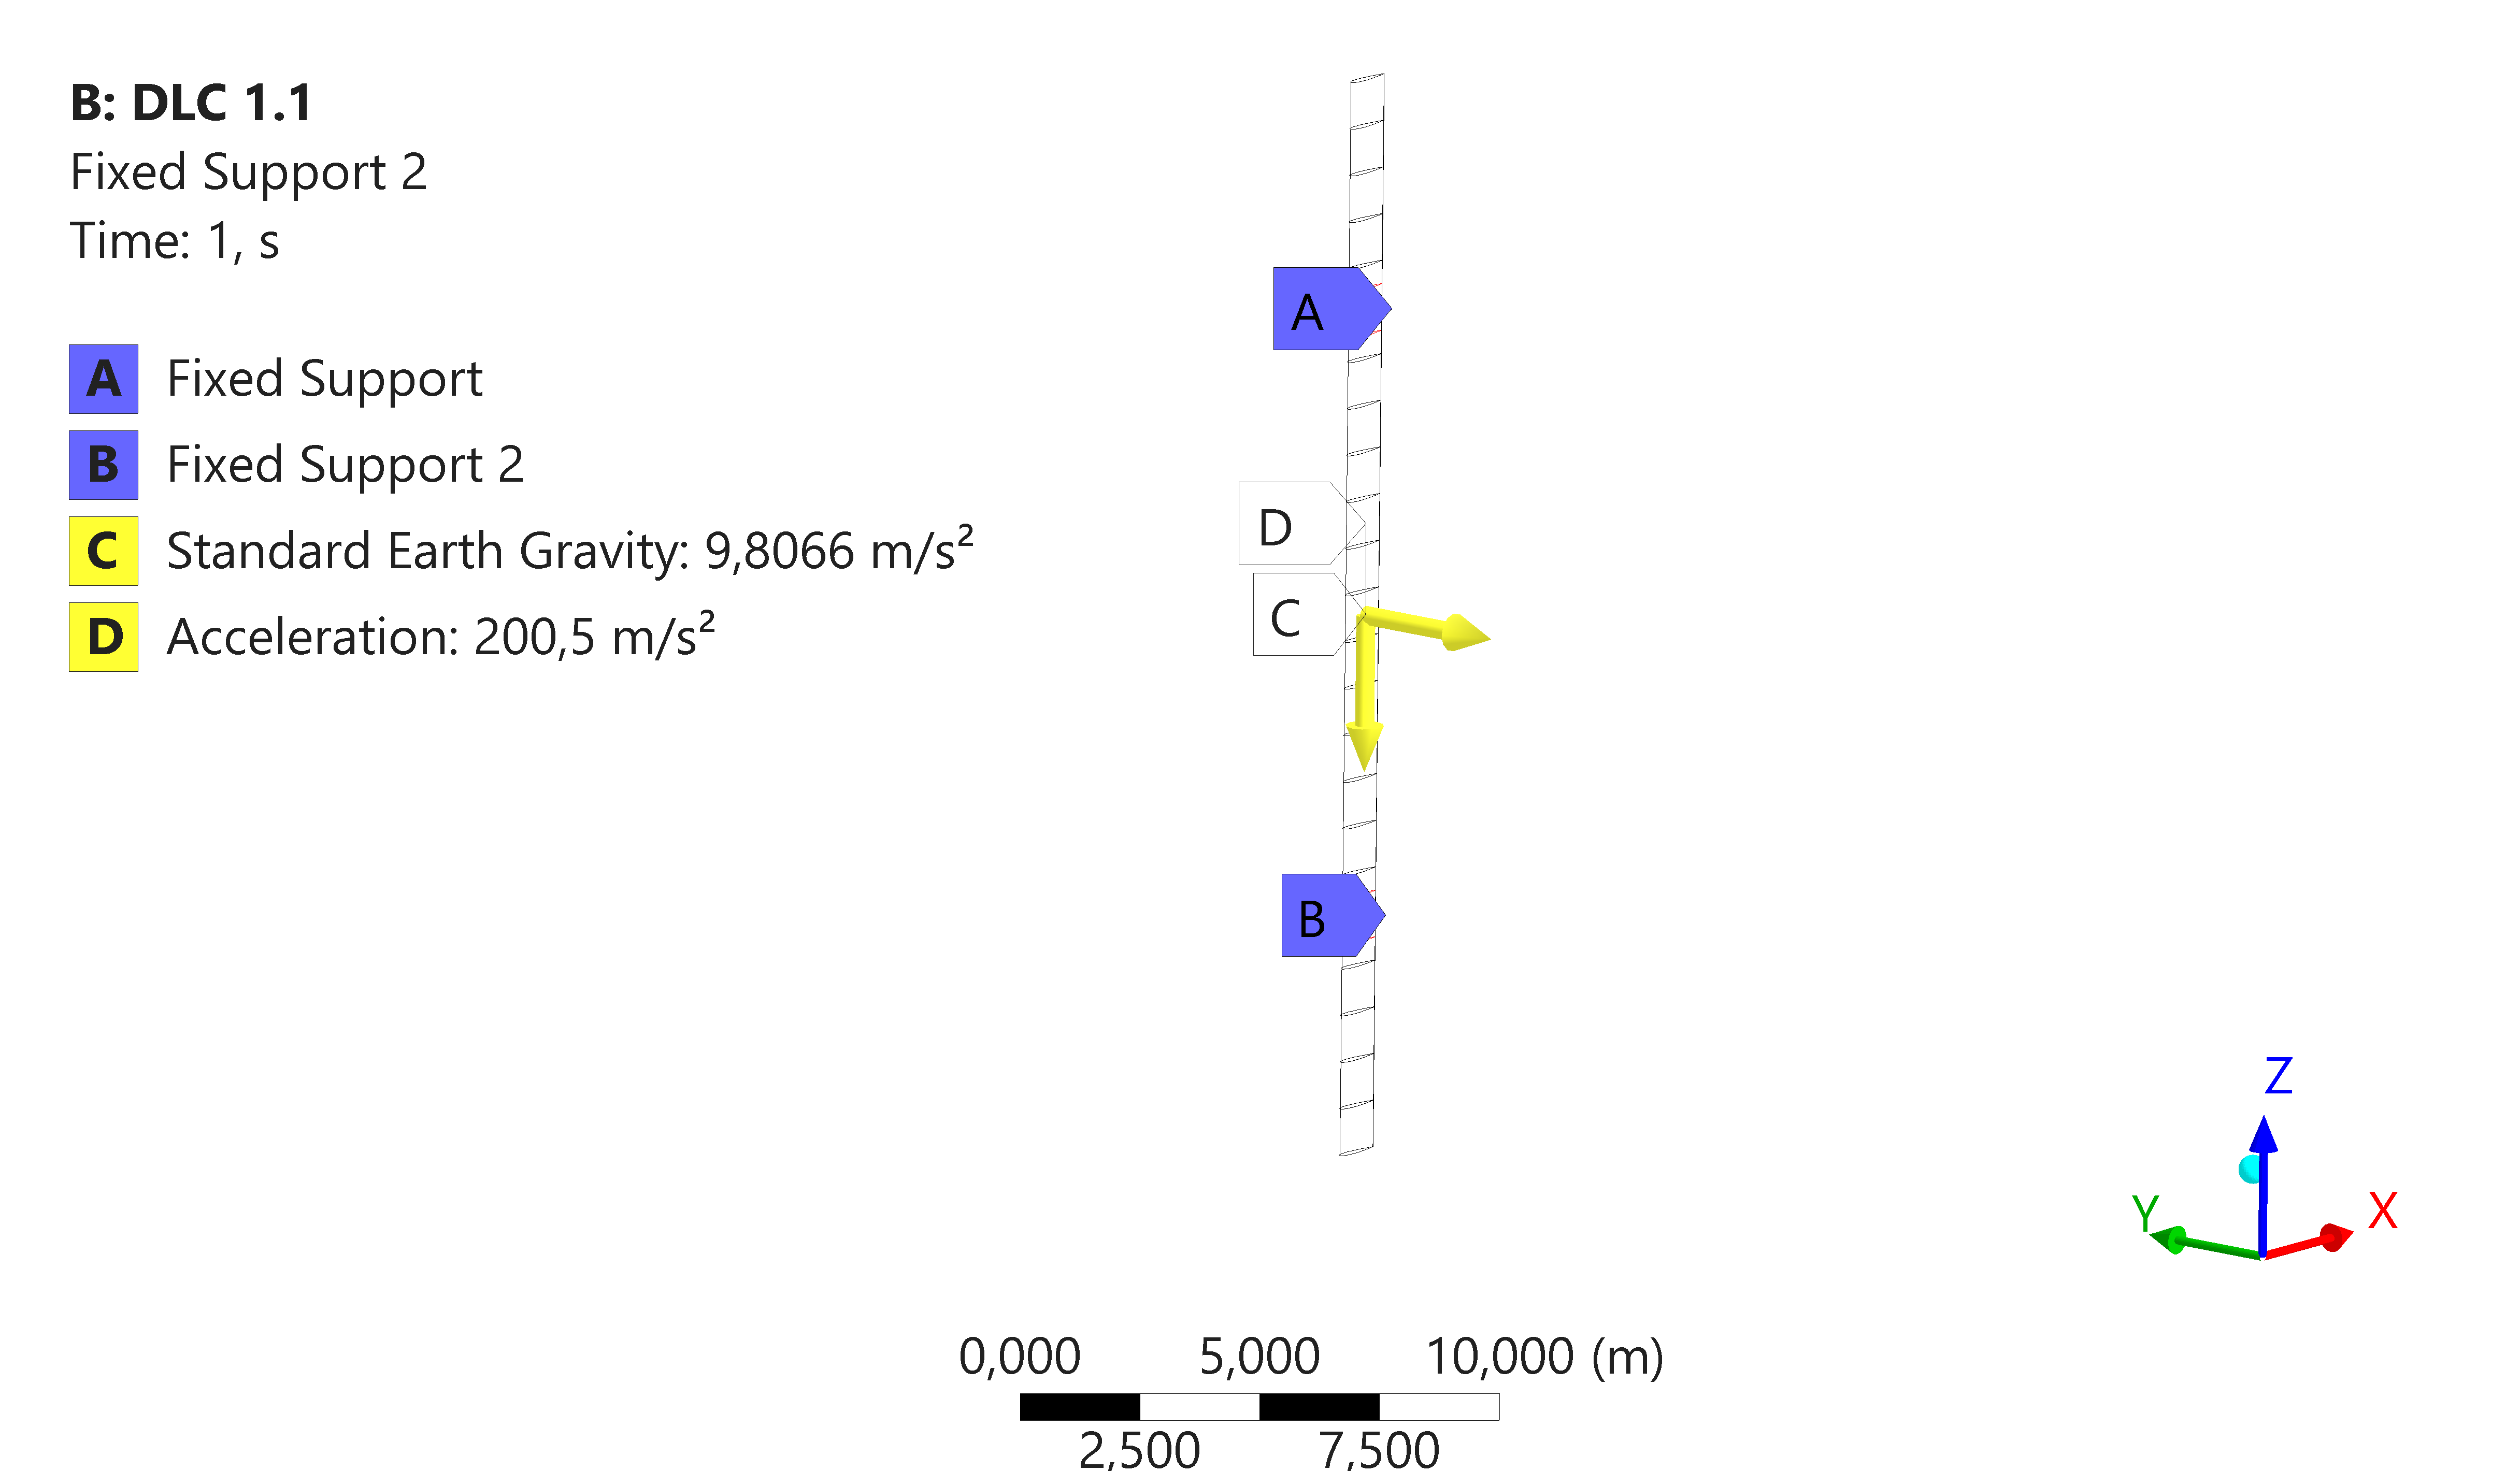
\includegraphics[width=\textwidth]{Figuras/Figuras Resultados/fem_cb.png}
    \caption{Condiciones de borde del modelo FEM, empotramientos en los dos puntos de conexión con los struts y aceleración centrífuga radial.}
    \label{fig:fem_cb}
\end{figure}

La aceleración centrífuga corresponde a la velocidad máxima de rotación $\Omega = 42$~rpm ($4{,}398$~rad/s) que, evaluada en la Ec.~\ref{eq:centrifugal_limit} con $R = 10{,}365$~m, resulta en $a_c = 200{,}5$~m/s$^2$ ($20{,}4\,g$), uniforme en toda la envergadura. Esa magnitud sitúa en su justa dimensión la consigna de $42$~rpm. Como la aceleración centrífuga es inversamente proporcional al radio (Ec.~\ref{eq:centrifugal_limit}), el menor radio del rotor en estudio implica una solicitación centrífuga un $29\%$ superior a la de la T1-turbine en su límite de diseño~\parencite{Mollerstrom2017}, pese a que ambas máquinas comparten la misma velocidad de punta. La admisibilidad de la consigna no se sustenta por tanto en la comparación con la literatura, sino en la verificación estructural que se desarrolla en esta sección.

La Figura~\ref{fig:fem_fuerzas} muestra las fuerzas aerodinámicas de diseño $F_d$ del DLC 1.1 aplicadas como cargas remotas en los centroides de las 24 estaciones, conservando el signo del instante gobernante (Sección~\ref{sec:anexo_f}), en el cual la componente normal a la cuerda apunta hacia el extradós, coincidiendo con el sentido de la flexión inducida por la fuerza centrífuga, condición que hace de este el estado combinado más desfavorable.

\begin{figure}[H]
    \centering
    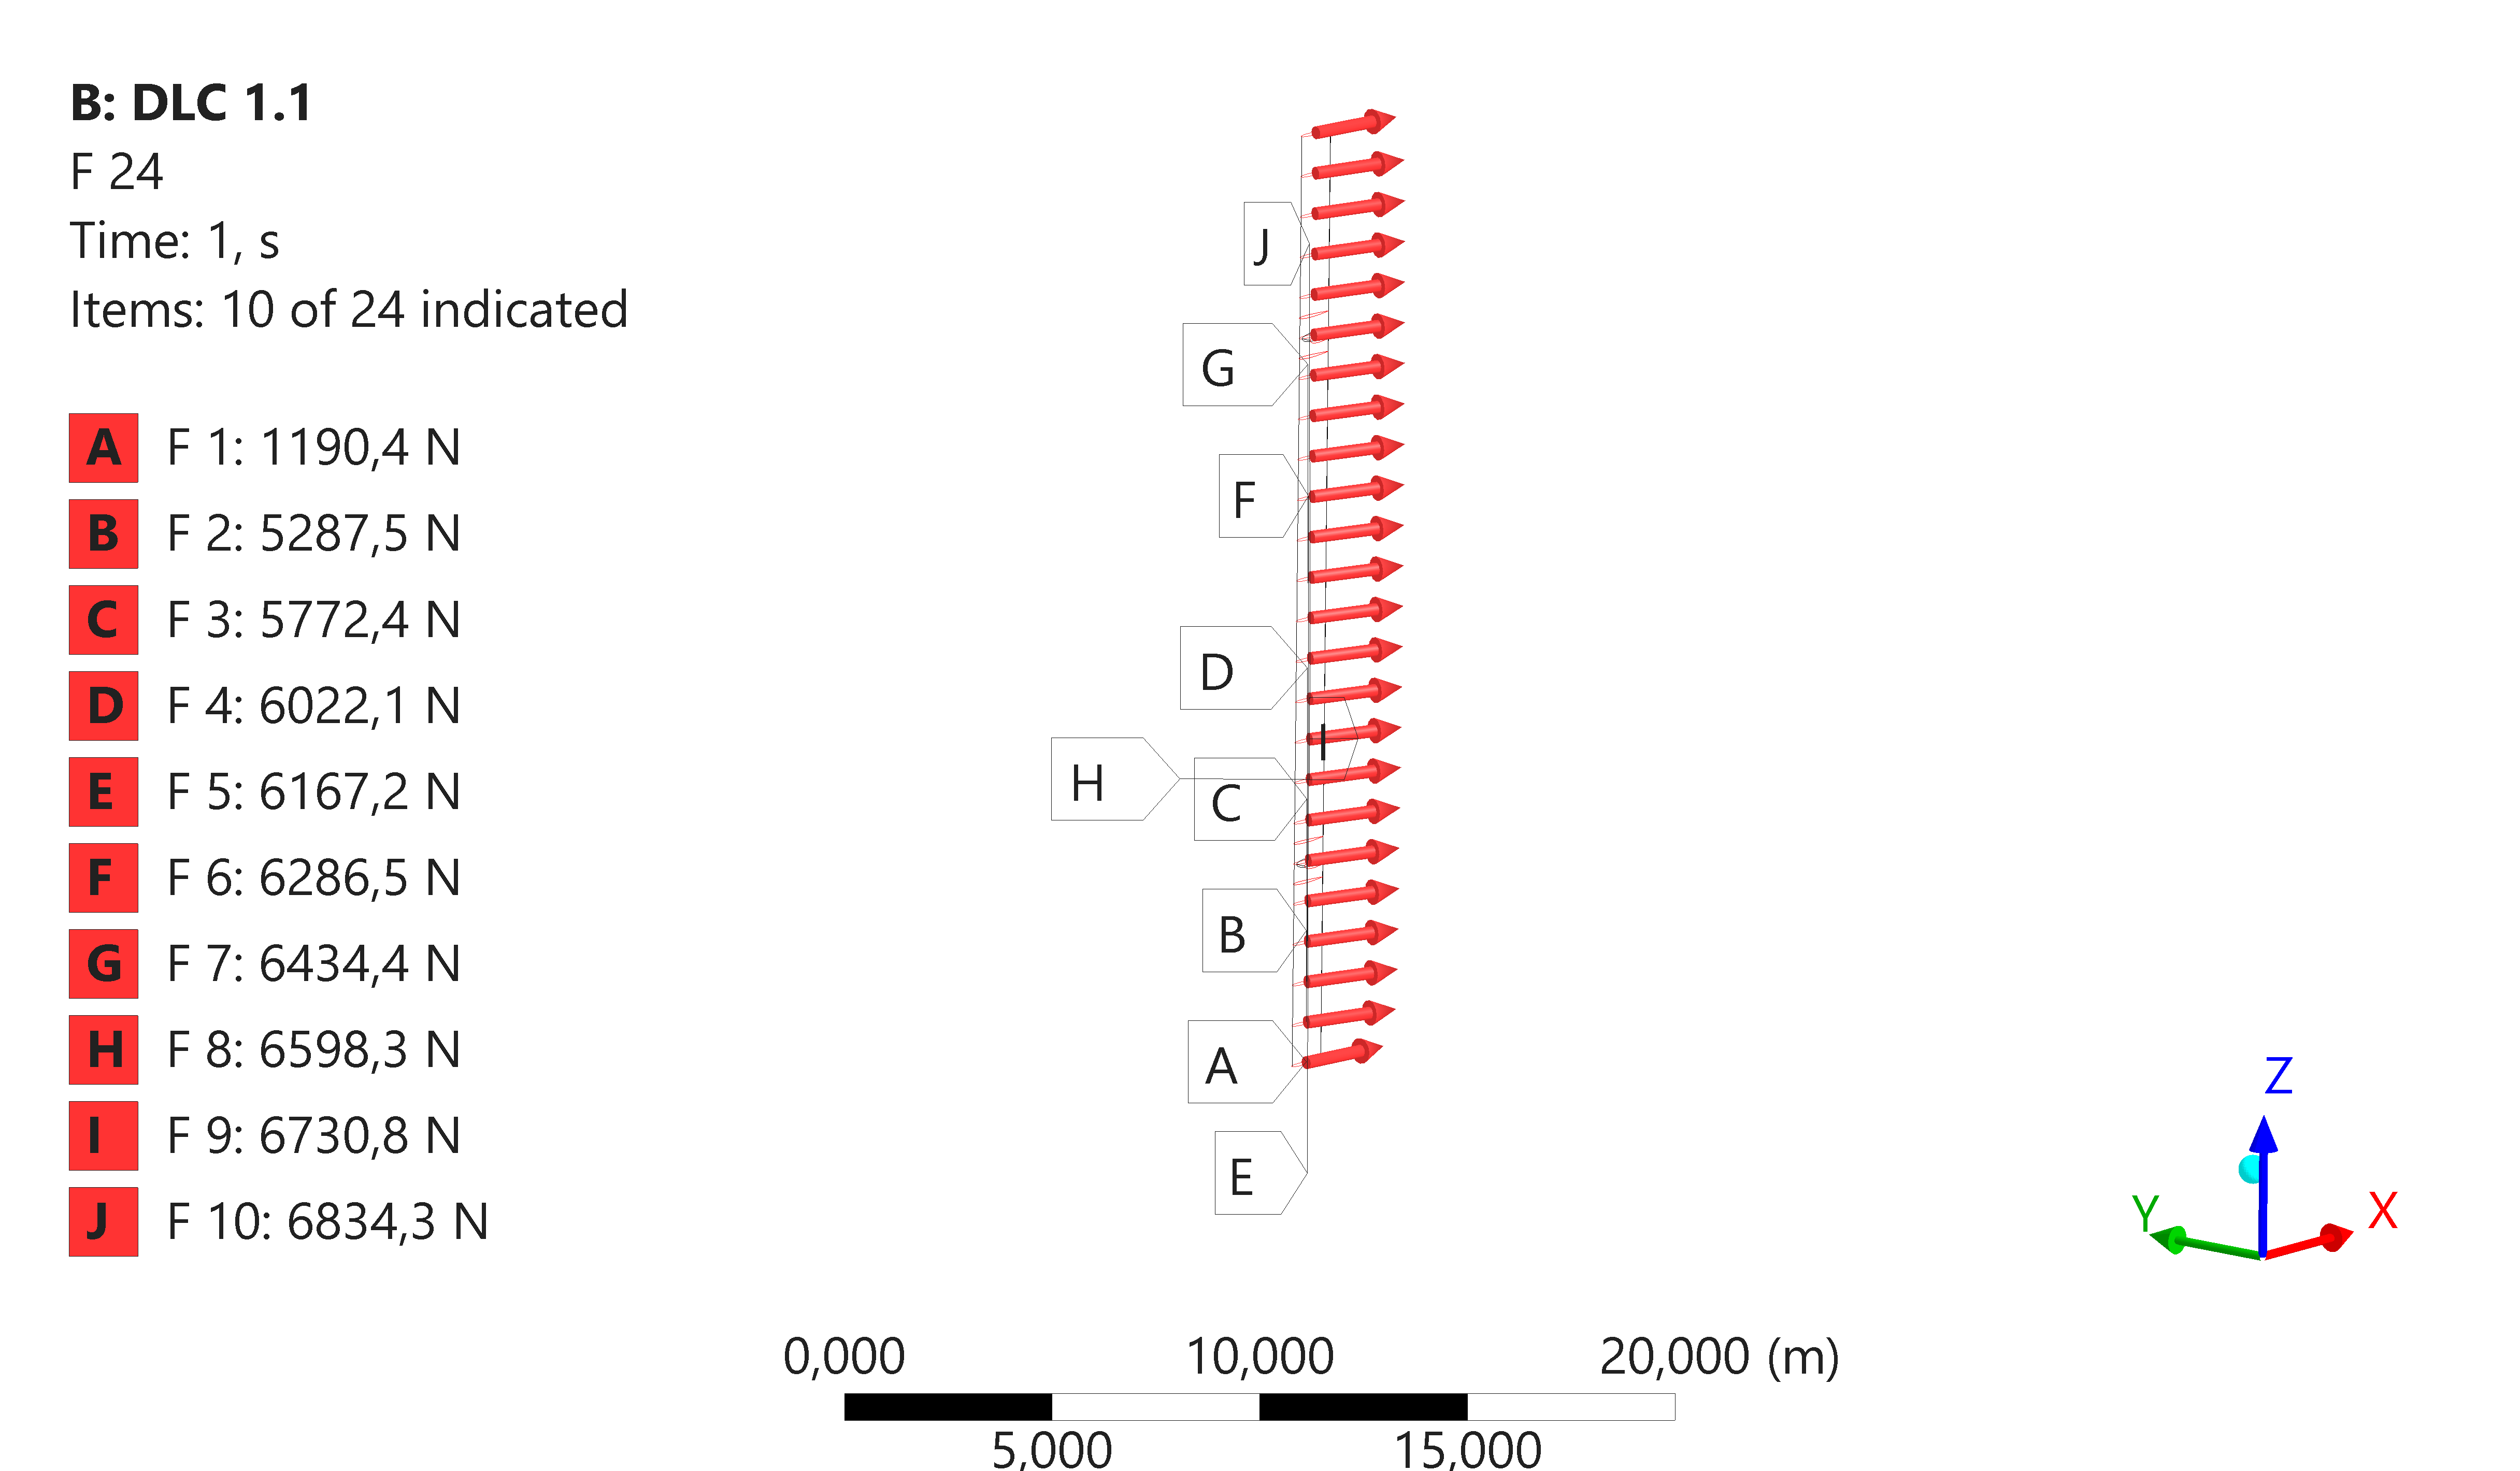
\includegraphics[width=\textwidth]{Figuras/Figuras Resultados/fem_fuerzas.png}
    \caption{Fuerzas aerodinámicas de diseño aplicadas como cargas remotas en las 24 estaciones de la pala.}
    \label{fig:fem_fuerzas}
\end{figure}

La Figura~\ref{fig:fem_detalle_union} presenta el detalle constructivo de la unión entre la pala y el brazo de soporte tal como queda resuelta en el modelo. Se distinguen en ella sus tres elementos, el vendaje de refuerzo de la zona de conexión y la superficie de apoyo sobre la que se imponen los empotramientos (Sección~\ref{sec:condiciones_borde}), y el larguero interior de $8$~mm alojado en la zona de espesor máximo del perfil (Sección~\ref{sec:material_pala}).


\begin{figure}[H]
    \centering
    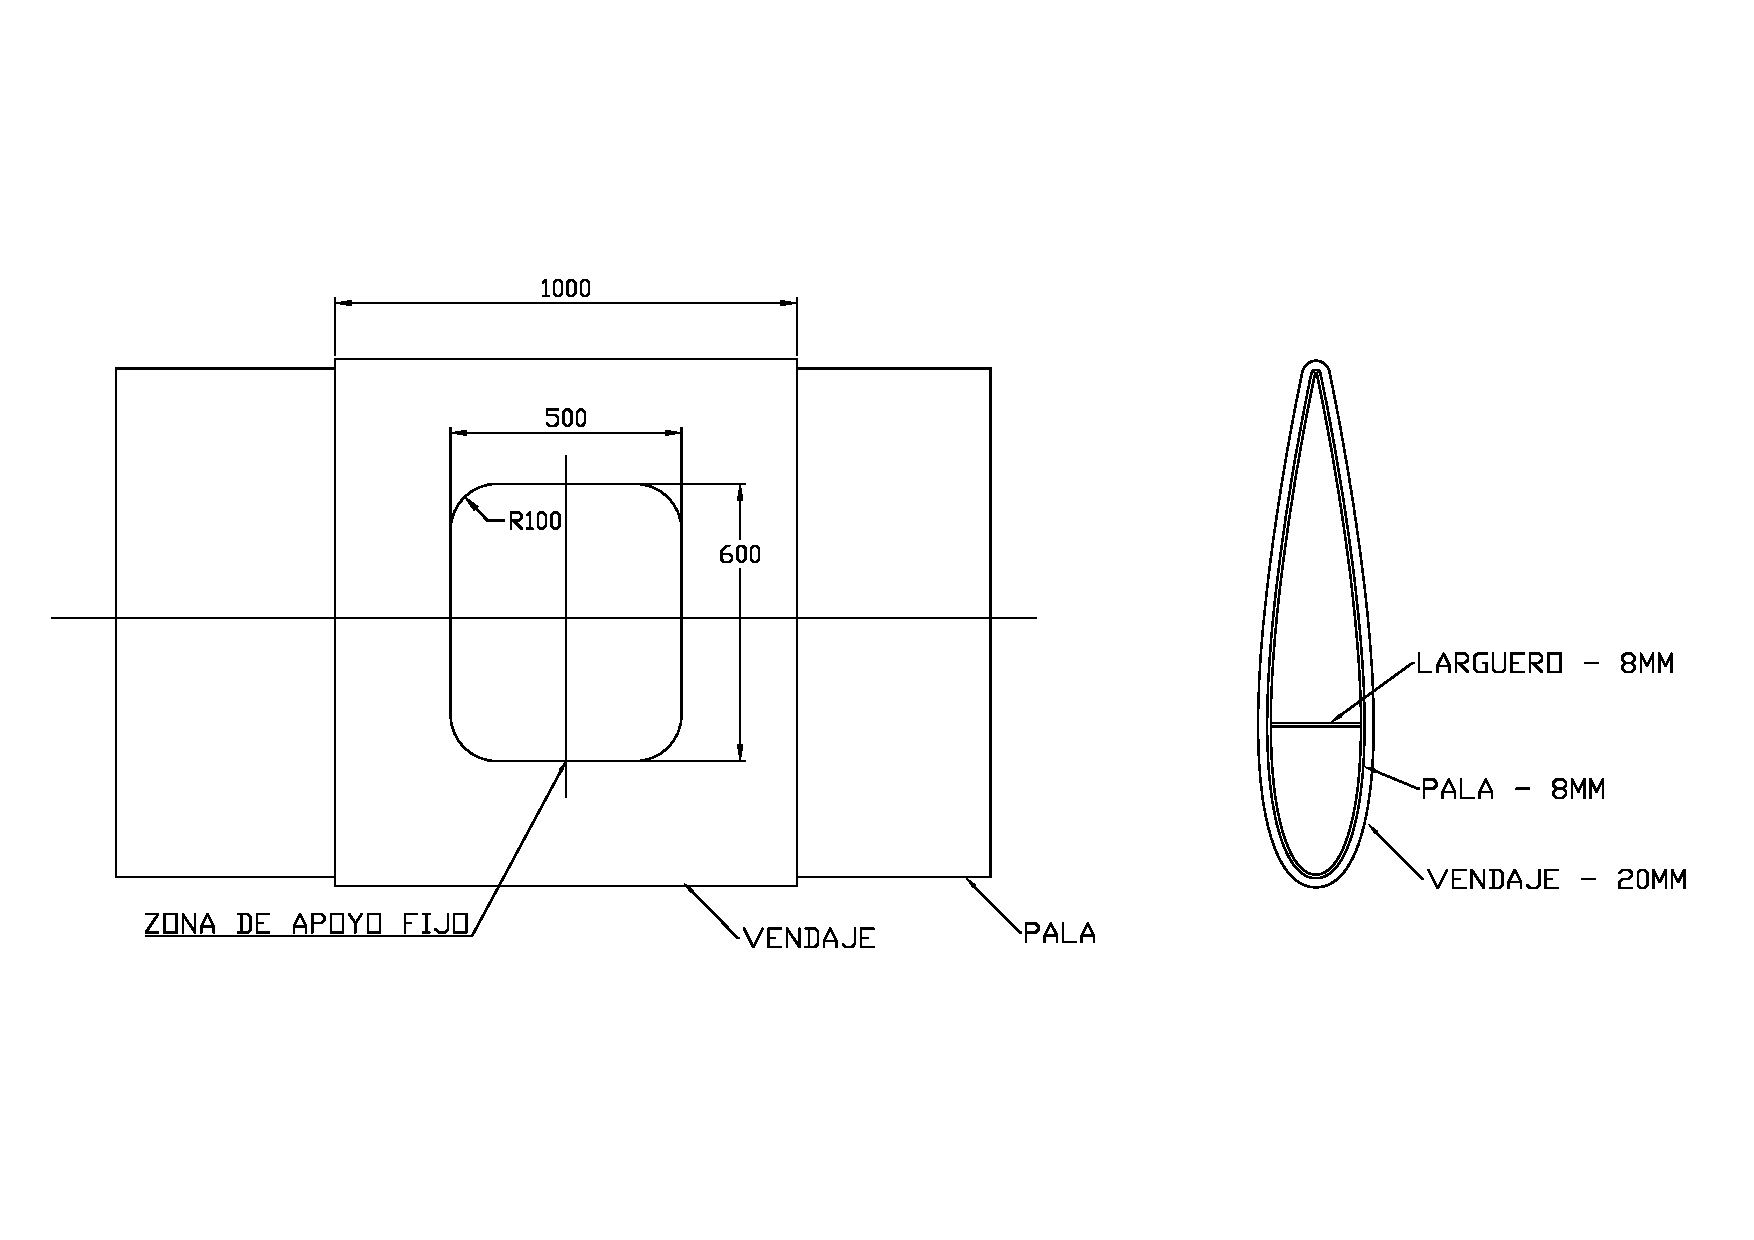
\includegraphics[trim=0cm 3cm 0cm 3cm, clip, width=0.85\textwidth]{Figuras/Figuras Resultados/PLANO.pdf}
    \caption{Detalle de la unión pala-brazo modelada en el FEM.}
    \label{fig:fem_detalle_union}
\end{figure}

\subsection{Resultados del análisis estructural}

Se reportan primero las tensiones y la deformación bajo las cargas del DLC 1.1, caso gobernante de la resistencia última, y a continuación las correspondientes al DLC 1.3. Adicionalmente, se presenta un caso de referencia resuelto únicamente con las cargas inerciales (aceleración centrífuga y gravedad, sin fuerzas aerodinámicas), que permite cuantificar la contribución de la rotación al estado tensional.

\subsubsection{Tensiones principales}

La Figura~\ref{fig:fem_max11} presenta la distribución de tensión principal máxima en ambas caras de la pala (intradós y extradós), junto con un detalle de la zona crítica. El valor máximo $\sigma_{1,\max} = 163{,}4$~MPa se localiza en la zona de conexión con el strut inferior ($z = 5$~m).

\begin{figure}[H]
    \centering
    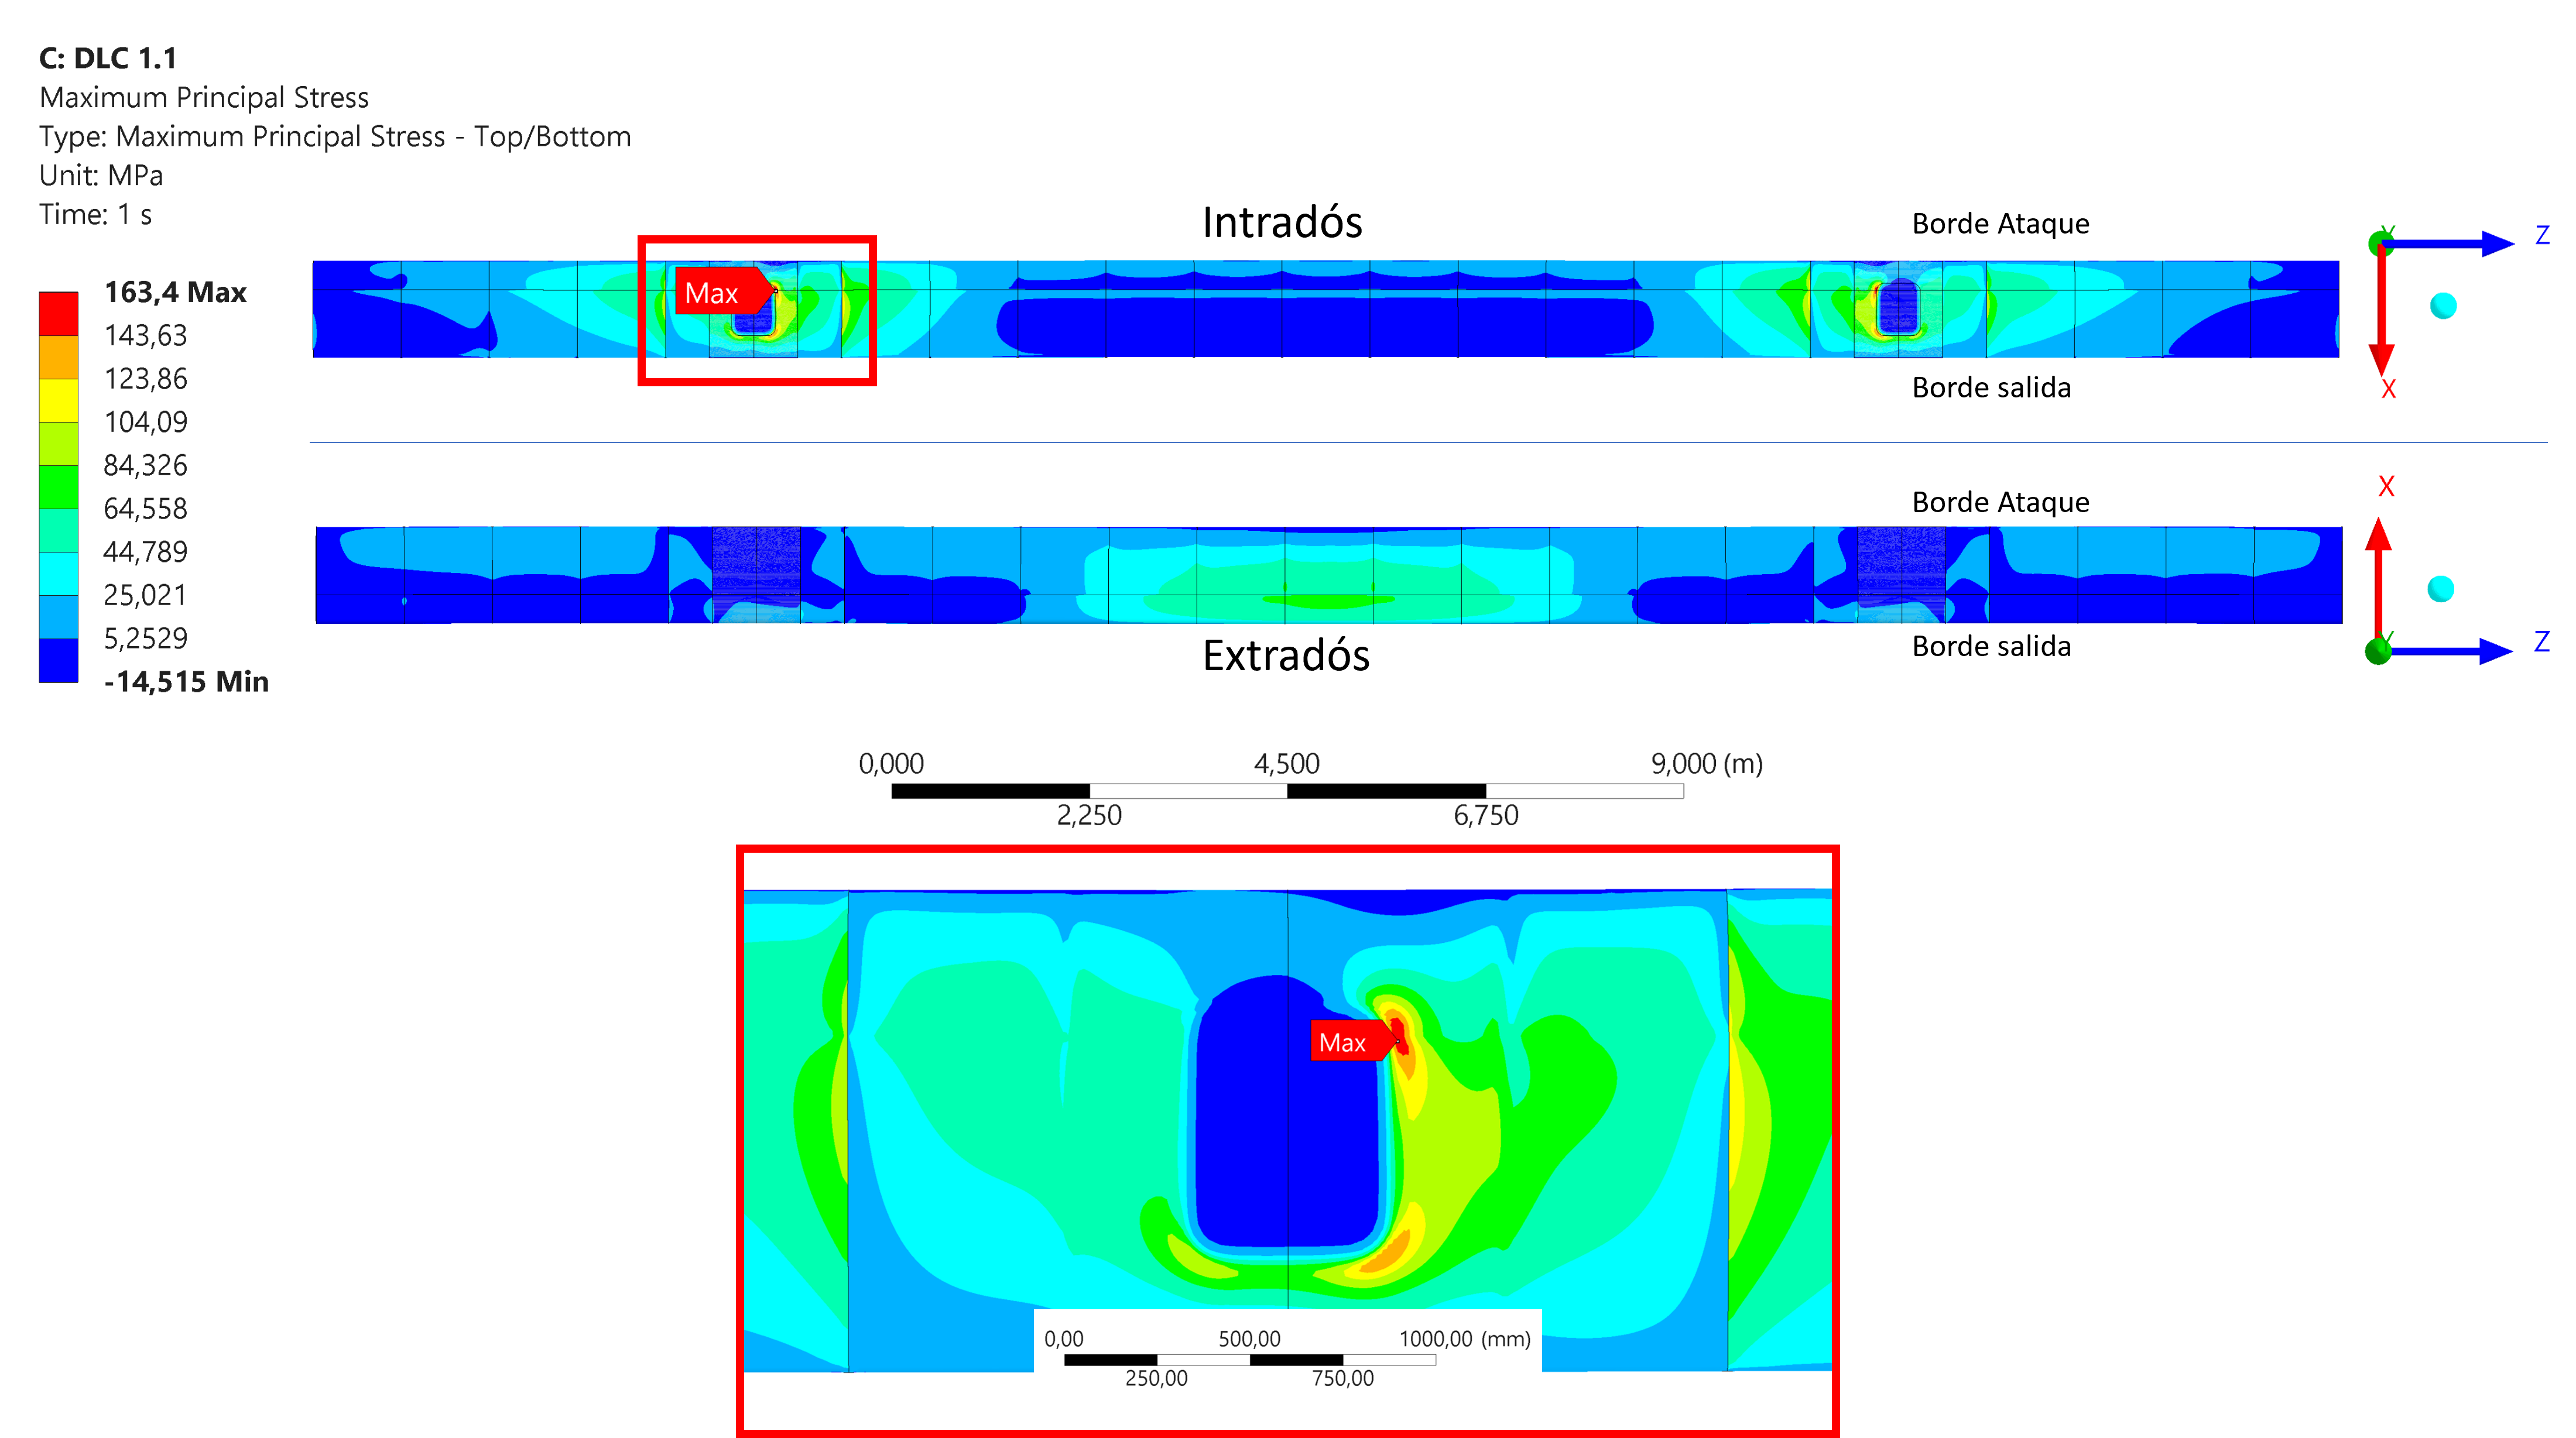
\includegraphics[width=\textwidth]{Figuras/Figuras Resultados/fem_max11.png}
    \caption{Distribución de tensión principal máxima, DLC 1.1.}
    \label{fig:fem_max11}
\end{figure}

Conviene precisar el alcance de ese valor. Ante la falta de un plano de la unión, el soporte se representó mediante una superficie de apoyo al final del brazo, reforzada por un vendaje (Sección~\ref{sec:condiciones_borde}), y es justamente en esa zona donde el modelo localiza el máximo. La tensión obtenida responde, por tanto, tanto a la solicitación como a la geometría supuesta para la unión. El análisis de convergencia descarta que el concentrador provenga de la discretización, ya que la tensión varía un $0{,}76\%$ entre las dos mallas más finas, pero no puede descartar su sensibilidad al detalle constructivo, ya que una unión de mayor superficie de apoyo, con una transición más gradual hacia el laminado, redistribuiría la tensión en esa zona.

La Figura~\ref{fig:fem_min11} muestra la tensión principal mínima, $\sigma_{3,\min} = -127{,}1$~MPa, correspondiente a compresión en la zona de las conexiones. Este estado de tracción en una cara y compresión en la opuesta responde a la flexión inducida por las fuerzas aerodinámicas y la fuerza centrífuga, que en el instante de diseño actúan en el mismo sentido (Sección~\ref{sec:anexo_f}).

\begin{figure}[H]
    \centering
    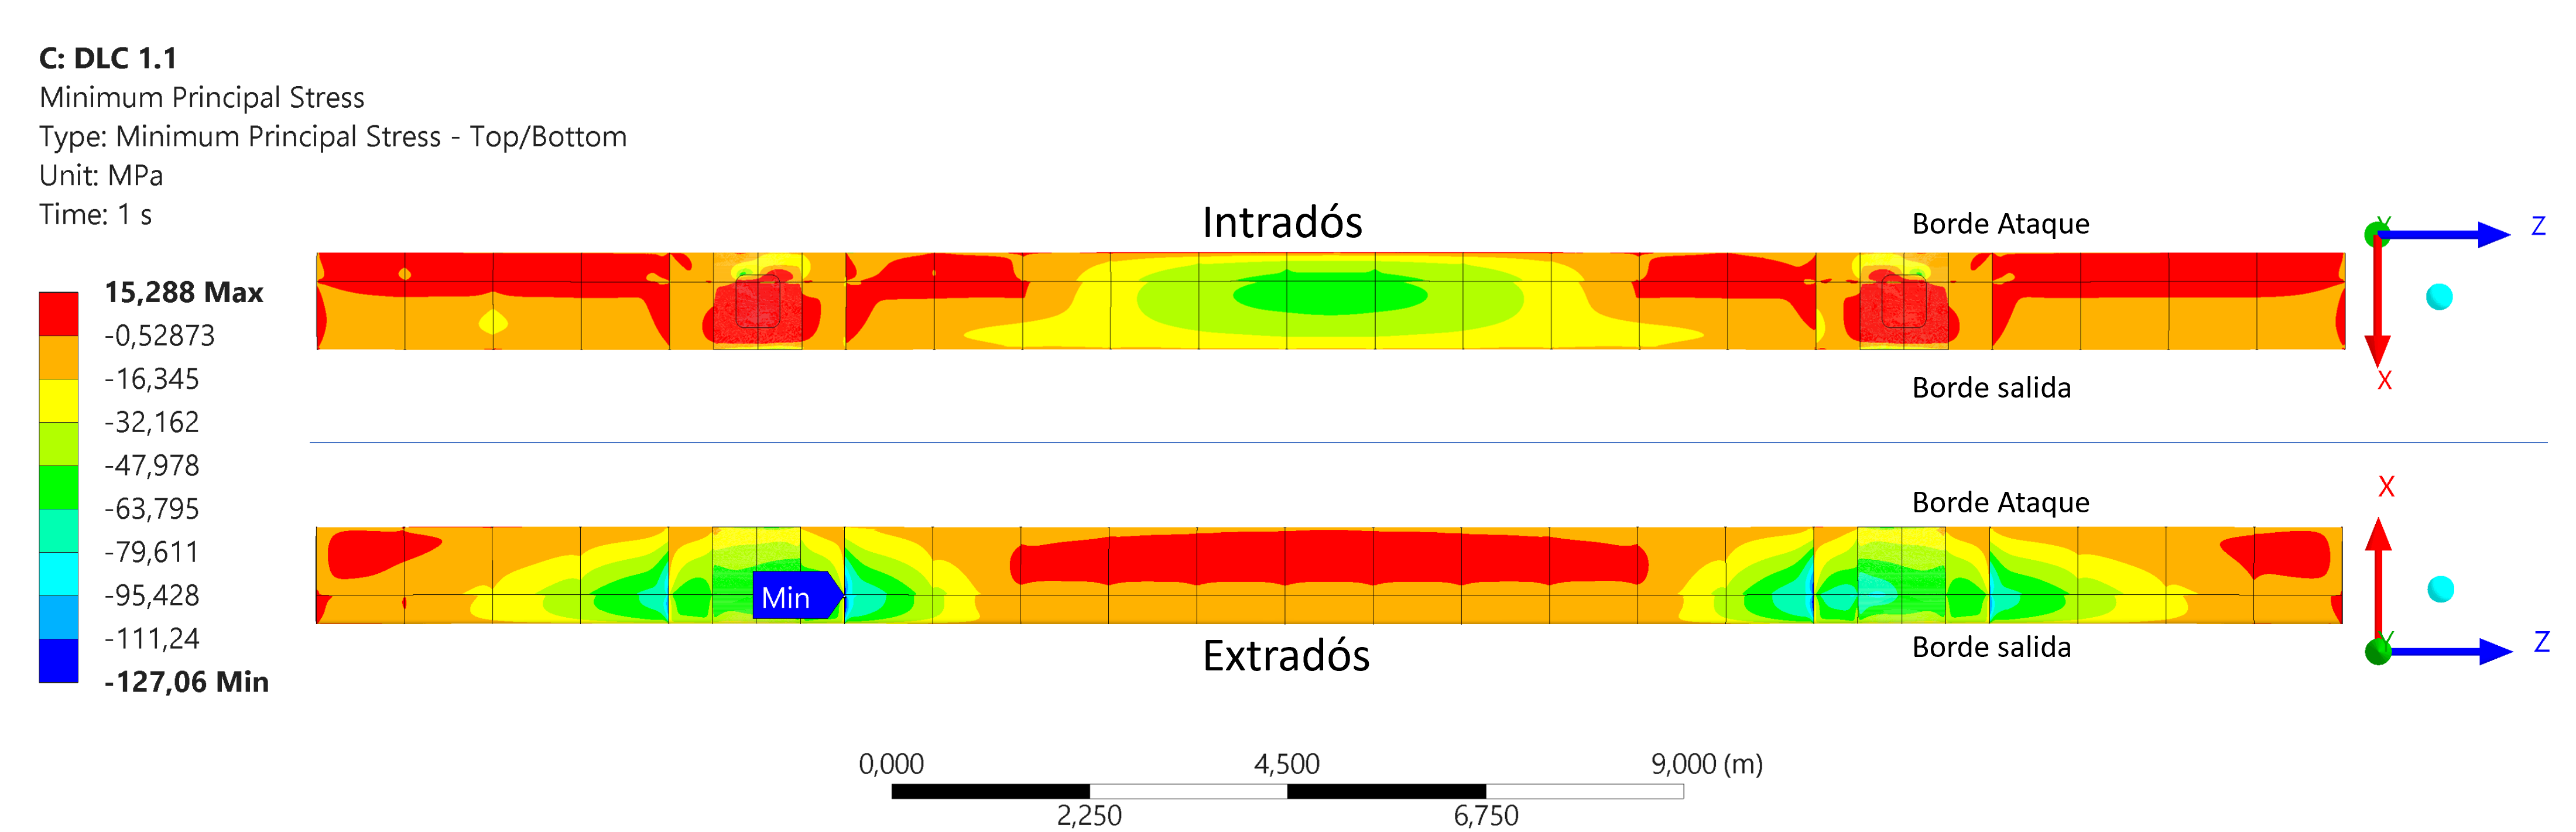
\includegraphics[width=\textwidth]{Figuras/Figuras Resultados/fem_min11.png}
    \caption{Distribución de tensión principal mínima, DLC 1.1.}
    \label{fig:fem_min11}
\end{figure}

\subsubsection{Deformación}

La Figura~\ref{fig:fem_deformacion11} presenta la deformación total de la pala bajo las cargas de diseño del DLC 1.1. La deformación máxima es de $0{,}169$~m y ocurre en la zona central de la pala, entre ambos apoyos, donde la flexión del vano alcanza su flecha máxima.

\begin{figure}[H]
    \centering
    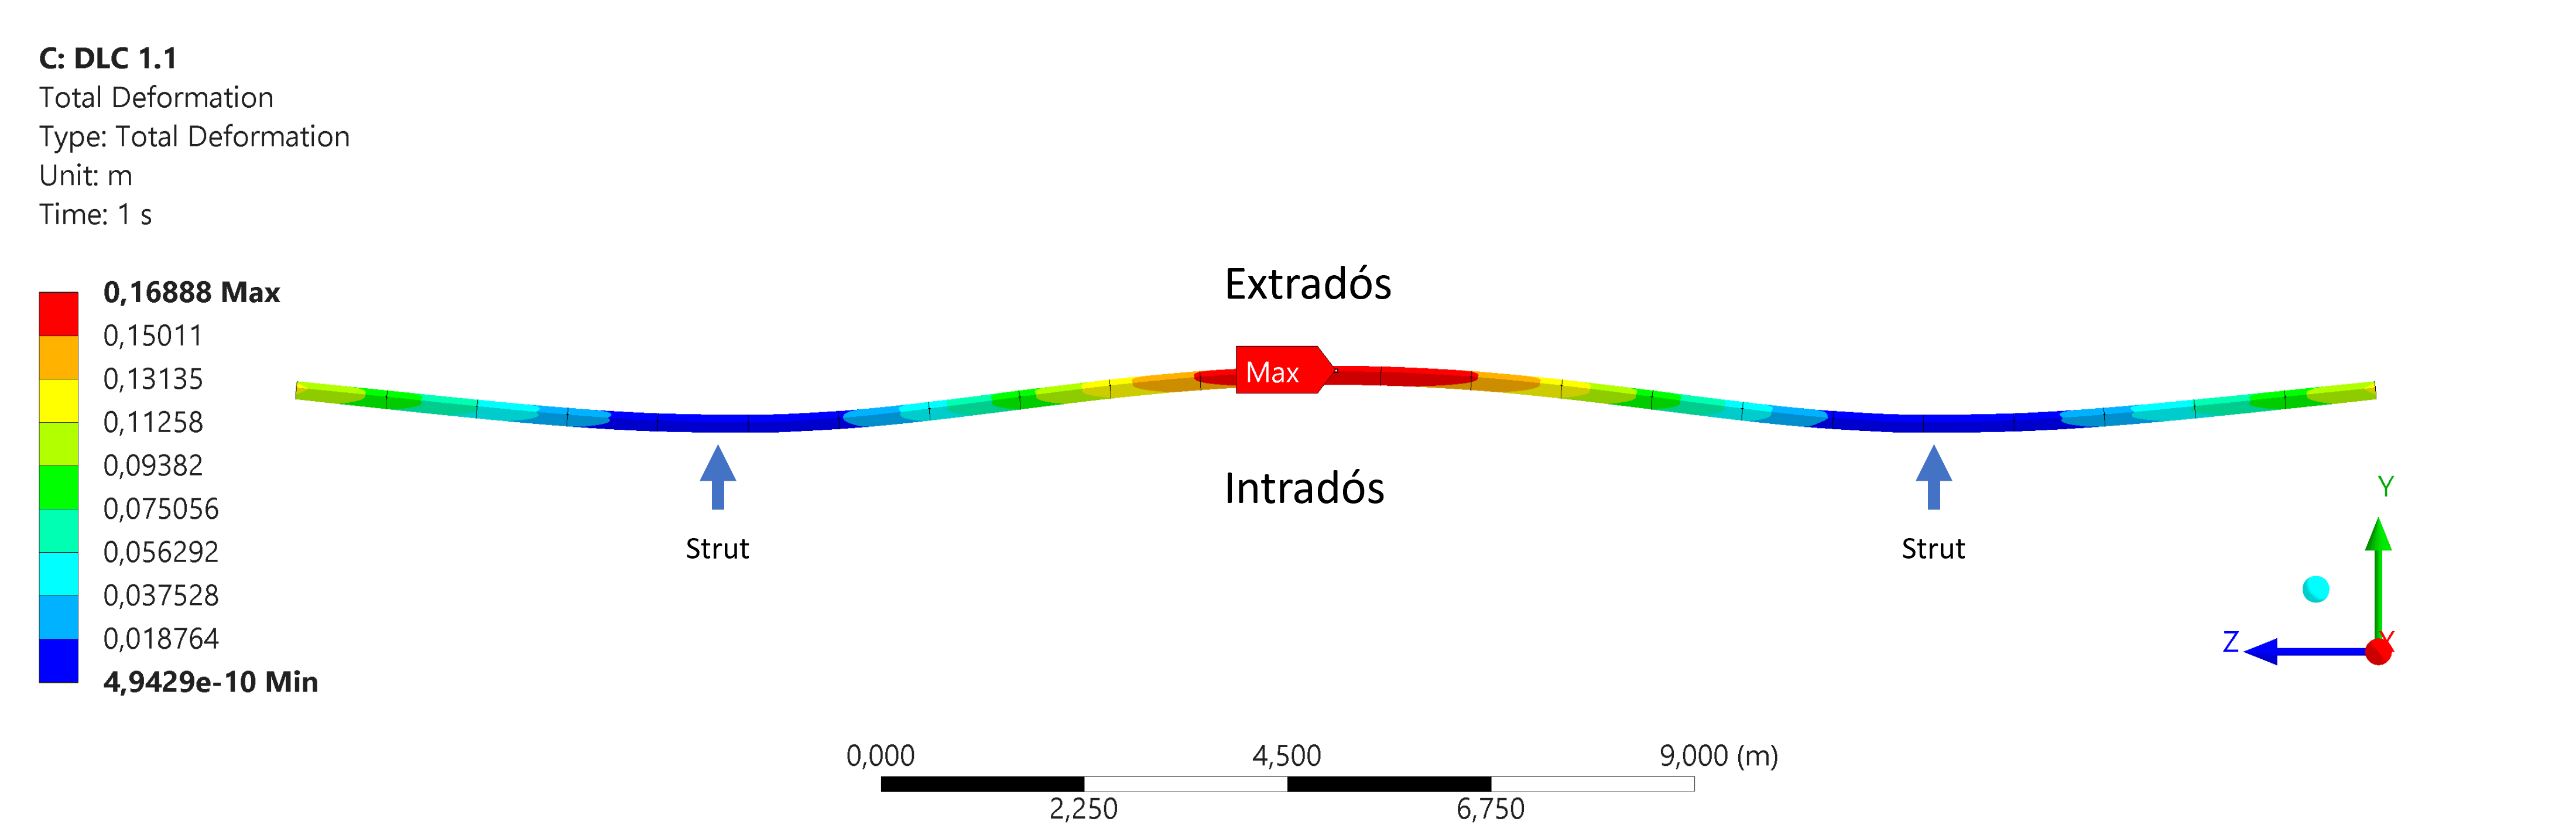
\includegraphics[width=\textwidth]{Figuras/Figuras Resultados/fem_deformacion11.png}
    \caption{Deformación total, DLC 1.1.}
    \label{fig:fem_deformacion11}
\end{figure}

\subsubsection{DLC 1.3}

Bajo las cargas de diseño del DLC 1.3, la distribución de tensión principal máxima (Figura~\ref{fig:fem_max13}) conserva el patrón del caso anterior, ya que el valor máximo, $\sigma_{1,\max} = 156{,}8$~MPa, vuelve a localizarse en la zona de las conexiones pala-brazo, lo que confirma que la ubicación de la sección crítica no depende del caso de carga.

\begin{figure}[H]
    \centering
    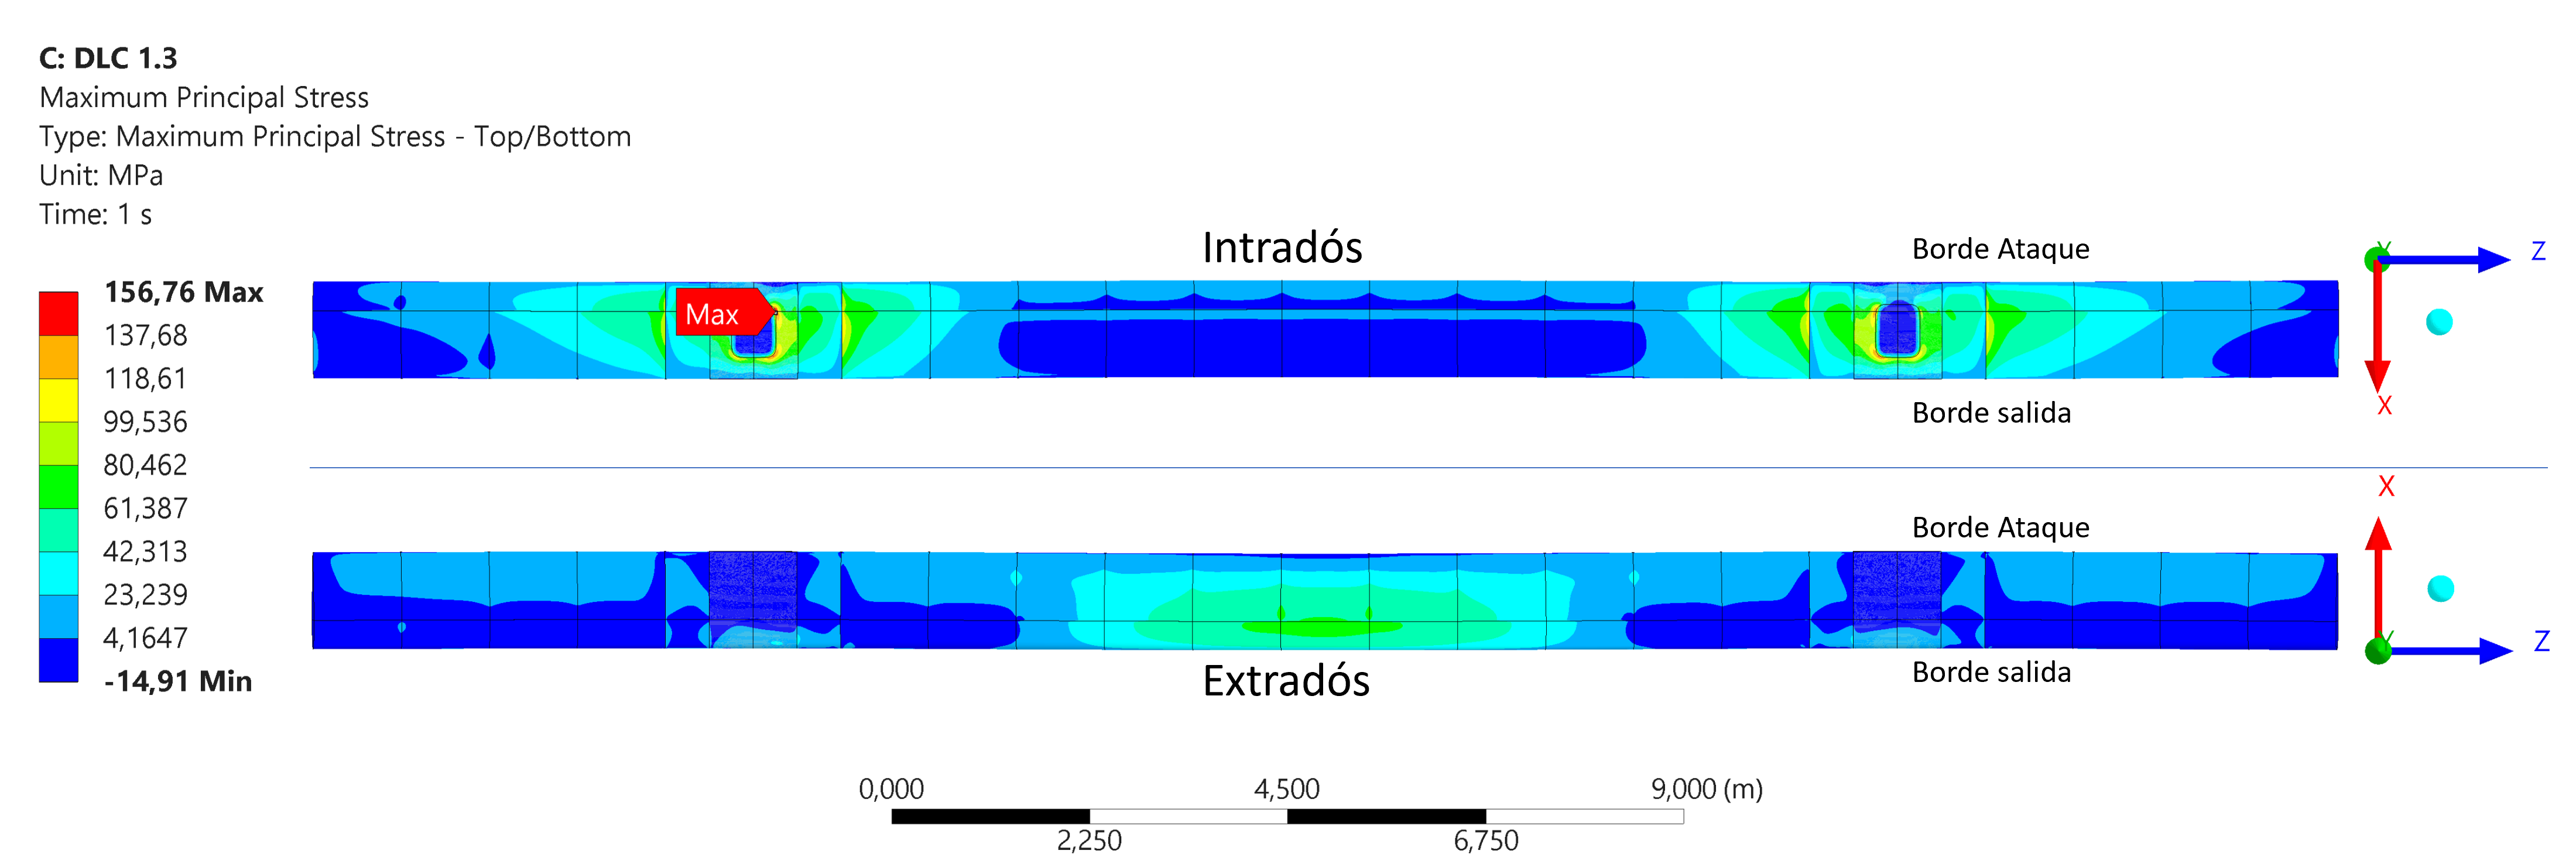
\includegraphics[width=\textwidth]{Figuras/Figuras Resultados/fem_max13.png}
    \caption{Distribución de tensión principal máxima, DLC 1.3.}
    \label{fig:fem_max13}
\end{figure}

En compresión, la tensión principal mínima (Figura~\ref{fig:fem_min13}) alcanza $\sigma_{3,\min} = -129{,}4$~MPa, en este caso de magnitud levemente mayor que la del DLC 1.1 ($-127{,}1$~MPa).

\begin{figure}[H]
    \centering
    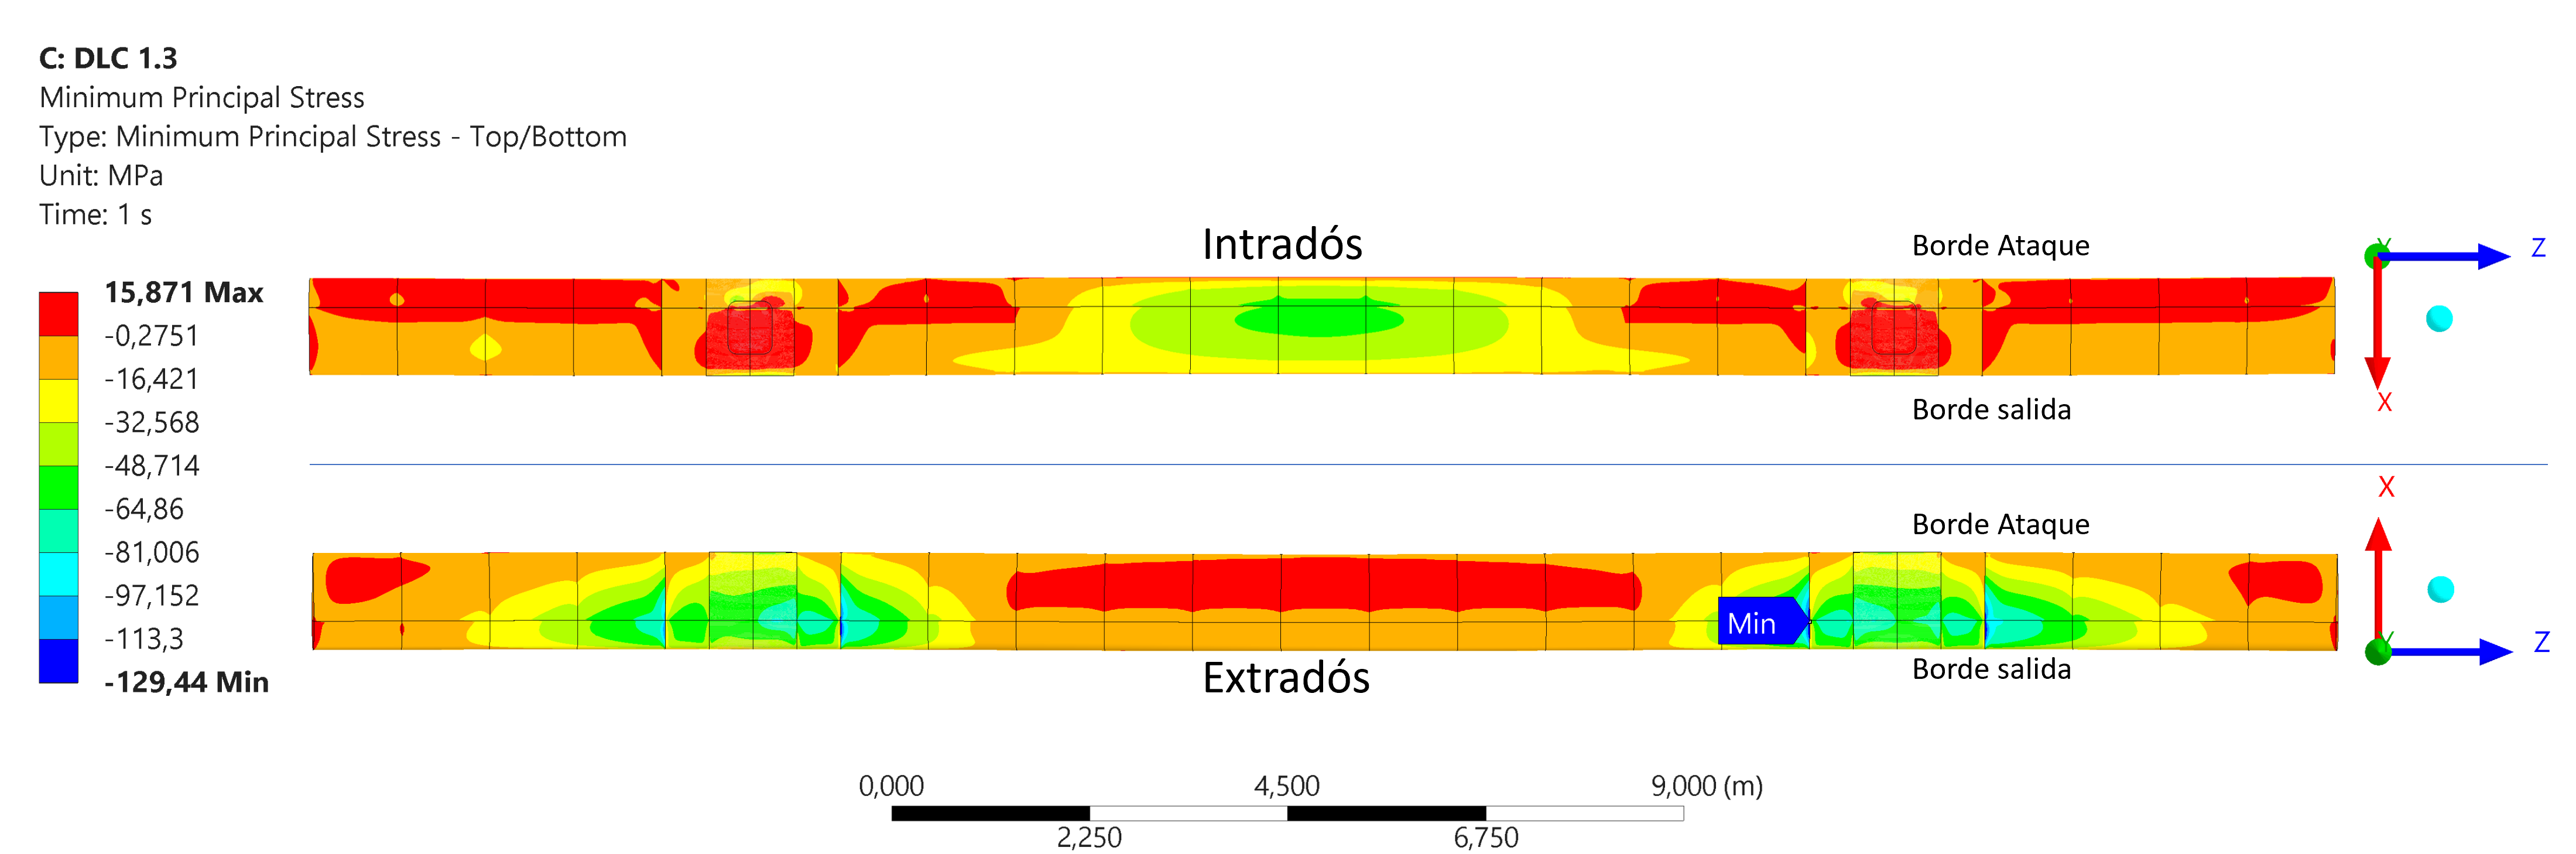
\includegraphics[width=\textwidth]{Figuras/Figuras Resultados/fem_min13.png}
    \caption{Distribución de tensión principal mínima, DLC 1.3.}
    \label{fig:fem_min13}
\end{figure}

La deformación total (Figura~\ref{fig:fem_deformacion13}) alcanza un máximo de $0{,}164$~m, nuevamente en la zona central entre apoyos.

\begin{figure}[H]
    \centering
    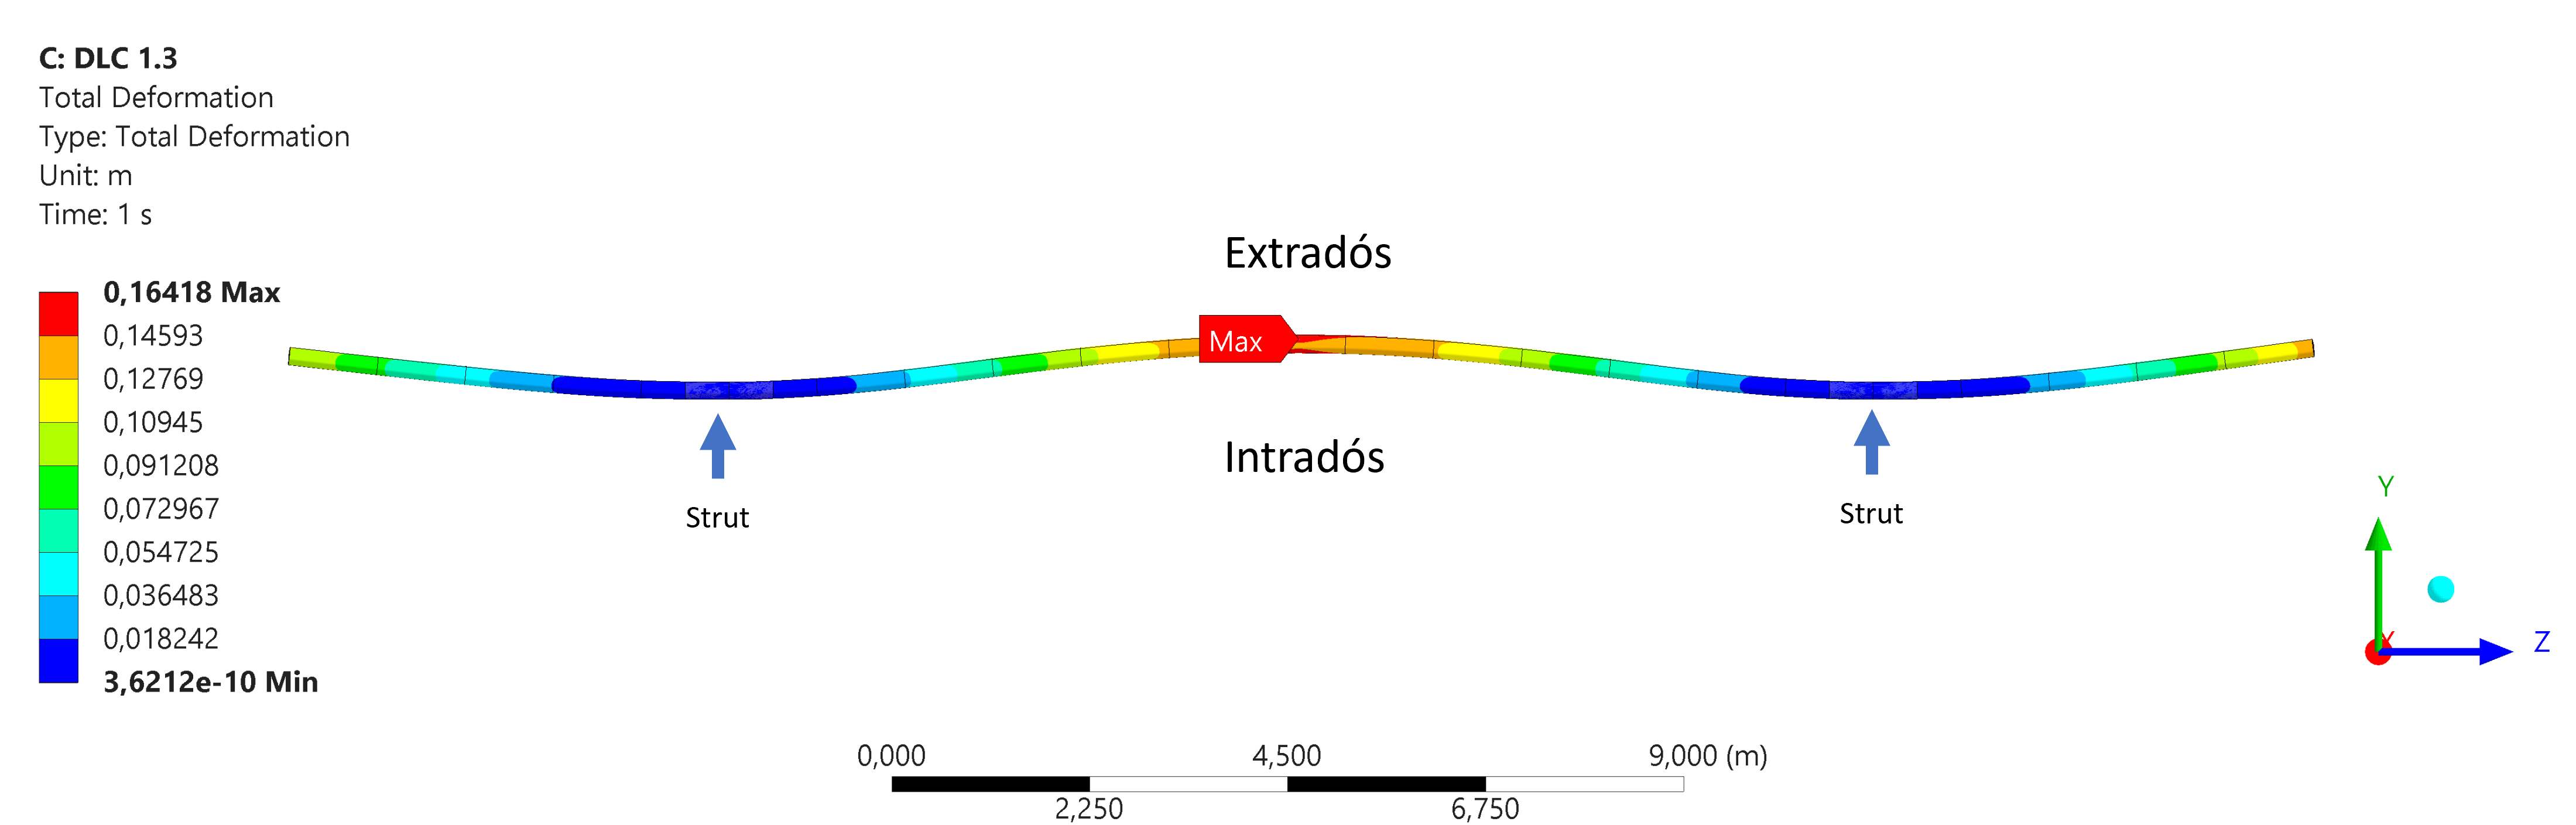
\includegraphics[width=\textwidth]{Figuras/Figuras Resultados/fem_deformacion13.png}
    \caption{Deformación total, DLC 1.3.}
    \label{fig:fem_deformacion13}
\end{figure}

Que la tensión máxima y la deformación resulten menores que en el DLC 1.1 pese a la mayor carga global tiene su origen en la distribución de las fuerzas. Ambos casos se resuelven con idénticas condiciones de borde y aceleraciones, por lo que la única diferencia entre ellos es el perfil de carga por estación. El DLC 1.1, extraído de un único instante de la simulación, concentra mayor carga en el vano central entre apoyos, cuya flexión solicita las conexiones y produce la flecha máxima del vano, mientras que el DLC 1.3, construido como media de máximos por estación, distribuye la carga de forma más suave hacia los voladizos (Sección~\ref{sec:comparacion_dlc}), lo que se refleja en una compresión levemente mayor pero una tracción y una deflexión menores.

\subsubsection{Contribución de las cargas inerciales}
\label{sec:solo_inercial}

Para cuantificar el peso de la rotación en el estado tensional, el modelo se resuelve adicionalmente con las cargas inerciales, aceleración centrífuga de $20{,}4\,g$ y gravedad, como única solicitación, sin fuerzas aerodinámicas. La tensión principal máxima resultante es $\sigma_{1,\max} = 114{,}5$~MPa en la misma zona crítica.

Este caso de referencia entrega una conclusión de diseño central, ya que la carga permanente de rotación produce por sí sola el $70\%$ de la tensión del caso gobernante ($114{,}5$ de $163{,}4$~MPa), mientras que el viento, incluso en su condición extrema de diseño a 50 años, aporta el $30\%$ restante. La pala está dimensionada principalmente por la fuerza centrífuga, es decir, por la decisión de control que fija la velocidad máxima de rotación en $42$~rpm, y no por el viento del emplazamiento. Este resultado también explica que las reacciones en los brazos apenas difieran entre ambos DLC, ya que la componente inercial, idéntica en los dos casos, domina el equilibrio global.

\subsubsection{Verificación de resistencia última}

La verificación de resistencia última emplea el criterio de máxima tensión principal, apropiado para materiales compuestos de matriz polimérica con comportamiento frágil~\parencite{Moraras2023}, según la Ec.~\ref{eq:criterio_uls}:

\begin{equation}
    \sigma_{1,\max} \leq \sigma_{u,d} = \frac{\sigma_u}{\gamma_m \cdot \gamma_n}
    \label{eq:criterio_uls}
\end{equation}

Con $\sigma_u = 242{,}1$~MPa, entregada por el fabricante de la pala (Tabla~\ref{tab:material_pala}), $\gamma_m = 1{,}30$ y $\gamma_n = 1{,}00$ según la Sección~\ref{sec:factores_seguridad}, la resistencia factoreada resulta según la Ec.~\ref{eq:sigma_ud_res}:

\begin{equation}
    \sigma_{u,d} = \frac{242{,}1}{1{,}30 \times 1{,}00} = 186{,}2\ \text{MPa}
    \label{eq:sigma_ud_res}
\end{equation}

Para el DLC 1.1, $\sigma_{1,\max} = 163{,}4$~MPa gobierna la verificación con un factor de reserva $\eta_{\text{ULS}}^{1.1} = 186{,}2 / 163{,}4 = 1{,}14$. Para el DLC 1.3, $\sigma_{1,\max} = 156{,}8$~MPa resulta en $\eta_{\text{ULS}}^{1.3} = 186{,}2 / 156{,}8 = 1{,}19$. Ambos casos satisfacen el criterio normativo, con márgenes del $14\%$ y el $19\%$ respectivamente.

En compresión, $\sigma_{3,\min} = -127{,}1$~MPa (DLC 1.1) y $-129{,}4$~MPa (DLC 1.3) se sitúan por debajo de la resistencia factoreada, por lo que esta verificación tampoco resulta condicionante en tensión; la relevancia de la compresión radica en la verificación de estabilidad que sigue.

\subsubsection{Verificación de estabilidad}

El análisis de pandeo lineal descrito en la Sección~\ref{sec:pandeo_met} se ejecuta sobre las soluciones estáticas de ambos casos de carga última. La Tabla~\ref{tab:pandeo} presenta los multiplicadores de carga de los tres primeros modos de cada caso.

\begin{table}[H]
    \centering
    \caption{Multiplicadores de carga del análisis de pandeo lineal.}
    \label{tab:pandeo}
    \begin{tabular}{ccc}
        \hline
        \textbf{Modo} & \textbf{$LM$, DLC 1.1} & \textbf{$LM$, DLC 1.3} \\
        \hline
        $1$ & $1{,}119$ & $1{,}131$ \\
        $2$ & $1{,}119$ & $1{,}131$ \\
        $3$ & $1{,}188$ & $1{,}167$ \\
        \hline
    \end{tabular}
\end{table}

Los modos corresponden a pandeo local de la piel de $8$~mm y se localizan en el vano central de la pala, en los paneles adyacentes al larguero, mecanismo característico de los cascarones de pared delgada de las palas de aerogenerador~\parencite{Boudounit2020}. El valor mínimo, $LM = 1{,}12$ (DLC 1.1), supera la unidad, por lo que el modelo no predice inestabilidad bajo la carga de diseño, pero no alcanza el umbral de $1{,}30$ de la Ec.~\ref{eq:criterio_pandeo}, por lo que la verificación de estabilidad no se satisface. Dado que el método lineal por autovalores constituye una cota superior de la carga crítica (Sección~\ref{sec:pandeo_met}), el margen faltante no es atribuible a conservadurismo del método.

Dos análisis de sensibilidad delimitan el origen del déficit. Primero, una configuración sin larguero interior resulta inviable, con multiplicadores inferiores a la unidad, lo que responde la pregunta de diseño planteada en la Sección~\ref{sec:material_pala}, ya que la omisión del larguero, alternativa que el fabricante evaluaba por facilidad de fabricación, no es estructuralmente viable con el espesor de piel estimado. Segundo, el aumento del espesor del larguero de $8$ a $12$~mm no modifica significativamente los multiplicadores, que se mantienen en torno a $1{,}1$. Este segundo resultado indica que el modo crítico está gobernado por los paneles de piel y no por el larguero. Una vez que este existe, seguir engrosándolo no aporta estabilidad, porque la capacidad de pandeo de un panel crece con el cuadrado de la razón entre su espesor y su ancho no apoyado (Ec.~\ref{eq:pandeo_placa}), y el larguero no modifica ninguna de las dos para los paneles adyacentes. En consecuencia, se mantiene el espesor de $8$~mm como configuración definitiva, y el cumplimiento del criterio de estabilidad queda supeditado a la rigidización de los paneles de piel, sea mediante elementos longitudinales adicionales (un segundo larguero o larguerillos), costillas transversales o un mayor espesor de piel en el vano central, alternativas cuya evaluación excede el alcance comprobatorio de este trabajo.

Que sea la estabilidad, y no la resistencia última, el criterio que no se satisface merece detenerse, porque no es el resultado que cabría anticipar. La razón es que ambos criterios interrogan propiedades distintas del laminado. La resistencia depende de cuánta tensión soporta el material, y en ella la pala conserva un factor de reserva de $1{,}14$; el pandeo depende de la rigidez del panel y de su geometría, y crece con el cuadrado de la razón entre el espesor de la piel y el ancho no apoyado (Ec.~\ref{eq:pandeo_placa}), de modo que un cascarón puede abollarse muy por debajo de la resistencia de su material.

Ese resultado señala, más que una deficiencia del diseño, el límite del modelo con que se lo evalúa, ya que tres de sus supuestos pesan directamente sobre él. El primero es el espesor de pared uniforme en todo el perímetro del perfil, adoptado al estimarlo desde la masa total de la pala (Sección~\ref{sec:material_pala}), cuando una distribución real concentraría material en las zonas de mayor solicitación y lo aligeraría en el resto. El segundo es la representación del laminado como un material isótropo equivalente, que no distingue la orientación del refuerzo, siendo que la carga crítica de un panel ortótropo depende de sus rigideces flexionales en cada dirección. El tercero es el propio larguero, cuyo espesor se igualó al del manto ante la falta de una definición del laminado. Los tres apuntan a que el margen obtenido debe leerse como una señal de que la sección requiere revisión, y no como una cuantificación exacta del déficit.

\subsubsection{Verificación de deflexiones}

La Sección 7.6.5 de la norma IEC 61400-1~\parencite{IEC61400-1} exige verificar que ninguna deflexión comprometa la integridad estructural ni produzca interferencia mecánica entre componentes. Para la configuración VAWT de palas rectas paralelas al eje de rotación, la deflexión radial no conlleva riesgo de impacto contra la torre. Las deflexiones máximas obtenidas del FEM bajo las cargas de diseño son $\delta_{\max} = 0{,}169$~m (DLC 1.1) y $0{,}164$~m (DLC 1.3), localizadas en el vano central entre apoyos. Referidas a la luz de dicho vano ($12$~m entre conexiones), representan una razón $\delta/L$ del $1{,}4\%$ en ambos casos. Estas deflexiones no comprometen la conexión con los struts ni el desempeño aerodinámico del rotor.

\subsection{Resumen de la verificación estructural}

La Tabla~\ref{tab:resumen_uls} sintetiza los resultados de la verificación a resistencia última para los DLC 1.1 y 1.3. La Tabla~\ref{tab:resumen_fatiga} presenta los resultados de la verificación a fatiga correspondiente al DLC 1.2.

\begin{table}[H]
    \centering
    \caption{Resumen de la verificación a fatiga.}
    \label{tab:resumen_fatiga}
    \begin{tabular}{llc}
        \hline
        \textbf{Símbolo} & \textbf{Descripción} & \textbf{DLC 1.2 (NTM)} \\
        \hline
        $\gamma_f$ & Factor parcial de carga & $1{,}00$ \\
        $\gamma_m \cdot \gamma_n$ & Factores parciales combinados & $1{,}96$ \\
        $\gamma_n$ & Factor de consecuencia (CC2, fatiga) & $1{,}15$ \\
        $K_{aero}$ & Factor de proporcionalidad momento-tensión & $0{,}752$~MPa/(kN$\cdot$m) \\
        $\sigma_{in}$ & Tensión media de origen inercial & $114{,}5$~MPa \\
        $D_{\text{año}}$ & Daño anual acumulado & $3{,}22 \times 10^{-9}$ \\
        $D_{20}$ & Daño acumulado en 20 años & $6{,}45 \times 10^{-8}$ \\
        \hline
    \end{tabular}
\end{table}

\begin{table}[H]
    \centering
    \caption{Resumen de la verificación a resistencia última.}
    \label{tab:resumen_uls}
    \begin{tabular}{llcc}
        \hline
        \textbf{Símbolo} & \textbf{Descripción} & \textbf{DLC 1.1 (NTM)} & \textbf{DLC 1.3 (ETM)} \\
        \hline
        \multicolumn{4}{c}{\textit{Cargas de diseño}} \\
        \hline
        $F_d$ & Carga de diseño global & $146{,}1$~kN & $152{,}1$~kN \\
        $F_{d,x}$ & Fuerza máx.\ por estación, eje $X_l$ & $6{,}78$~kN/m & $6{,}71$~kN/m \\
        $F_{d,y}$ & Fuerza máx.\ por estación, eje $Y_l$ & $2{,}40$~kN/m & $2{,}30$~kN/m \\
        $\gamma_f$ & Factor parcial de carga & $1{,}25$ & $1{,}35$ \\
        \hline
        \multicolumn{4}{c}{\textit{Tensiones (FEM)}} \\
        \hline
        $\sigma_{1,\max}$ & Tensión principal máxima & $163{,}4$~MPa & $156{,}8$~MPa \\
        $\sigma_{3,\min}$ & Tensión principal mínima & $-127{,}1$~MPa & $-129{,}4$~MPa \\
        \hline
        \multicolumn{4}{c}{\textit{Verificación del factor de seguridad}} \\
        \hline
        $\sigma_u/(\gamma_m \gamma_n)$ & Resistencia factoreada & $186{,}2$~MPa & $186{,}2$~MPa \\
        $\gamma_m$ & Factor parcial de material & $1{,}30$ & $1{,}30$ \\
        $\gamma_n$ & Factor de consecuencia de falla & $1{,}00$ & $1{,}00$ \\
        $\eta_{\text{ULS}}$ & Factor de reserva ($\sigma_u/(\gamma_m \gamma_n)/\sigma_{1,\max}$) & $1{,}14$ & $1{,}19$ \\
        \hline
        \multicolumn{4}{c}{\textit{Estabilidad (FEM)}} \\
        \hline
        $LM$ & Multiplicador de carga mínimo (modo 1) & $1{,}119$ & $1{,}131$ \\
        \hline
        \multicolumn{4}{c}{\textit{Deformación (FEM)}} \\
        \hline
        $\delta_{\max}$ & Deformación máxima & $0{,}169$~m & $0{,}164$~m \\
        --- & Ubicación & Centro & Centro \\
        \hline
    \end{tabular}
\end{table}

Los factores de reserva obtenidos ($\eta_{\text{ULS}} \geq 1{,}14$) y el daño acumulado por fatiga ($D_{20} = 6{,}45 \times 10^{-8} \ll 1{,}0$) confirman que la pala satisface los criterios normativos de resistencia última y fatiga establecidos en IEC 61400-1~\parencite{IEC61400-1}, y las deformaciones máximas se mantienen dentro de márgenes que no comprometen la operación del rotor. La verificación de estabilidad, en cambio, no se satisface, ya que el multiplicador de carga mínimo ($LM = 1{,}12 < 1{,}30$) muestra que el pandeo local de los paneles de piel gobierna el diseño. El caso de referencia con cargas exclusivamente inerciales cuantifica además que el $70\%$ de la tensión del caso gobernante proviene de la rotación, resultado que vincula el dimensionamiento estructural con la estrategia de control y que se desarrolla en el Capítulo~5.
